\documentclass[11pt,fleqn]{article}
\usepackage[margin=1in,top=1in,bottom=1in]{geometry}
\usepackage{tikz}
\usepackage{mathtools}
\usepackage{longtable}
\usepackage{enumitem}
\usepackage{hyperref}
%\usepackage[dvips]{graphics}
%\usepackage[table]{xcolor}
%\usepackage{amssymb}
\usepackage{float}
%\usepackage{subfig}
\usepackage{booktabs}
\usepackage{subcaption}

\usepackage[normalem]{ulem}

\usepackage{multicol}
\usepackage{txfonts}
\usepackage{amsfonts}
\usepackage{natbib}
\usepackage{gb4e}
\usepackage[all]{xy}
\usepackage{rotating}
\usepackage{tipa}
\usepackage{multirow}
\usepackage{authblk}
\usepackage{url}
\usepackage{pdflscape}
\usepackage{rotating}
\usepackage{adjustbox}
\usepackage{array}

\def\bad{{\leavevmode\llap{*}}}
\def\marginal{{\leavevmode\llap{?}}}
\def\verymarginal{{\leavevmode\llap{??}}}
\def\swmarginal{{\leavevmode\llap{4}}}
\def\infelic{{\leavevmode\llap{\#}}}

\definecolor{airforceblue}{rgb}{0.36, 0.54, 0.66}
%\definecolor{gray}{rgb}{0.36, 0.54, 0.66}

\definecolor{Pink}{RGB}{240,0,120}
\newcommand{\red}[1]{\textcolor{Pink}{#1}}
\newcommand{\jd}[1]{\textbf{\textcolor{Pink}{[jd: #1]}}}

\newcommand{\dashrule}[1][black]{%
  \color{#1}\rule[\dimexpr.5ex-.2pt]{4pt}{.4pt}\xleaders\hbox{\rule{4pt}{0pt}\rule[\dimexpr.5ex-.2pt]{4pt}{.4pt}}\hfill\kern0pt%
}

\setlength{\parindent}{.3in}
\setlength{\parskip}{0ex}

\newcommand{\yi}{\'{\symbol{16}}}
\newcommand{\nasi}{\~{\symbol{16}}}
\newcommand{\hina}{h\nasi na}
\newcommand{\ina}{\nasi na}

\newcommand{\foc}{$_{\mbox{\small F}}$}

\hyphenation{par-ti-ci-pa-tion}

\setlength{\bibhang}{0.5in}
\setlength{\bibsep}{0mm}
\bibpunct[:]{(}{)}{,}{a}{}{,}

\newcommand{\6}{\mbox{$[\hspace*{-.6mm}[$}} 
\newcommand{\9}{\mbox{$]\hspace*{-.6mm}]$}}
\newcommand{\sem}[2]{\6#1\9$^{#2}$}
\renewcommand{\ni}{\~{\i}}

\newcommand{\citepos}[1]{\citeauthor{#1}'s \citeyear{#1}}
\newcommand{\citeposs}[1]{\citeauthor{#1}'s}
\newcommand{\citetpos}[1]{\citeauthor{#1}'s (\citeyear{#1})}

\newcolumntype{R}[2]{%
    >{\adjustbox{angle=#1,lap=\width-(#2)}\bgroup}%
    l%
    <{\egroup}%
}
\newcommand*\rot{\multicolumn{1}{R{90}{0em}}}% no optional argument here, please!


\title{Are there factive predicates? An empirical investigation}

%\thanks{For helpful comments on the research presented here, we thank David Beaver, Cleo Condoravdi, Kai von Fintel, Lauri Karttunen, Mandy Simons, Greg Scontras, the anonymous reviewers for {\em Semantics and Linguistic Theory} 2018, as well as the audiences at the MIT Linguistics colloquium, the 2018 Annual Meeting of XPRAG.de and at the University of T\"ubingen. We gratefully acknowledge financial support for this research from {\em National Science Foundation} grant BCS-1452674 (JT) and the Targeted Investment for Excellence Initiative at The Ohio State University (JT). IGOR Tuebingen, SALT TALK}}

\author{Author(s)}

%\author[$\circ$]{Judith Tonhauser}
%\author[$\bullet$]{Judith Degen}
%\affil[$\circ$]{The Ohio State University / University of Stuttgart}
%\affil[$\bullet$]{Stanford University}
%
%\renewcommand\Authands{ and }

\newcommand{\jt}[1]{\textbf{\color{blue}JT: #1}}

\begin{document}

%\tableofcontents
%\newpage

\maketitle

\vspace*{-1cm}

\begin{abstract}

Properties of the content of the clausal complement have long been assumed to distinguish factive predicates like {\em know} from non-factive ones like {\em think} (\citealt{kiparsky-kiparsky70}, i.a.). There is, however, disagreement about which properties define factive predicates as well as uncertainty about whether the content of the complement of particular predicates exhibit the properties attributed to the content of the complement of factive predicates. This has led to a lack of consensus about which predicates are factive, a troublesome situation given the central role that factivity plays in linguistic theorizing. This paper reports six experiments designed to investigate two critical properties of the content of the complement of clause-embedding predicates, namely projection and entailment, with the goal of establishing whether these properties identify a class of factive predicates. We find that factive predicates are more heterogeneous than previously assumed and that there is little empirical support \jt{from these experiments} for the assumed categorical distinction between factive and non-factive predicates. We discuss implications of our results for formal analyses of presuppositions, one area where factivity has played a central role. We propose that projection is sensitive to more fine-grained meaning distinctions between clause-embedding predicates than factivity. \jt{(Word count of main text: 18,137)}

\end{abstract}

%Submissions to the journal must not exceed 18,000 words of main text inclusive of notes.
		
\section{Introduction}\label{s1}

Clause-embedding predicates are predicates like {\em know} and {\em think} that take a finite clause as an argument, as shown in (\ref{kk0}), where the finite clause {\em (that) it is raining} realizes the direct object. \citealt{kiparsky-kiparsky70} proposed that there is a  class of clause-embedding predicates called `factive' predicates, like {\em know}, that distinguish themselves from other predicates, like {\em think}, in that the content of their clausal complement is presupposed, that is, ``[t]he speaker presupposes that the embedded clause expresses a true proposition'' (p.147). Thus, a speaker who utters (\ref{kk0}) with {\em know} is taken to presuppose that it is raining, in contrast to a speaker who utters (\ref{kk0}) with {\em think}.

\begin{exe}
\ex\label{kk0} Sam \{ knows / thinks \} that it is raining.
\end{exe}
To diagnose whether a predicate is factive, that is, whether the content of its complement (henceforth CC) is presupposed, \citealt{kiparsky-kiparsky70} relied on the projection diagnostic (see also, e.g., \citealt{langendoen-savin71}). Specifically, they assumed that the CC of a clause-embedding predicate is presupposed if the speaker is committed to the truth of the CC not only when uttering an affirmative matrix sentence like (\ref{kk0}) but also when uttering negated or polar question variants of the affirmative matrix sentence, like those in (\ref{kk1}a) and (\ref{kk1}b), respectively. Thus, {\em know} was categorized in \citealt{kiparsky-kiparsky70} as a factive predicate because a speaker is committed to the CC when uttering the affirmative sentence in (\ref{kk0}) with {\em know} and when uttering its negated variant in (\ref{kk1}a) or the polar question variant in (\ref{kk1}b). By contrast, {\em think} was categorized as non-factive because the CC is not presupposed, that is, a speaker who utters the variants in (\ref{kk0}) and (\ref{kk1}a-b) with {\em think} is not necessarily committed to the truth of the CC.\footnote{Factive predicates were also taken to be distinguished by syntactic properties in \citealt{kiparsky-kiparsky70}. We ignore syntax here because \citet[fn.3]{kiparsky-kiparsky70} already pointed out that syntactic and semantic factivity are not perfectly aligned: {\em know} and {\em realize}, for instance, were taken to be syntactically non-factive but semantically factive. For recent discussion see \citealt{white-rawlins-nels2018}, \citealt{djaerv-thesis} and references therein.}  


\begin{exe}
\ex\label{kk1}
\begin{xlist}
\ex Sam doesn't \{ know / think  \} that it is raining.
\ex Does Sam \{ know / think  \} that it is raining?
\end{xlist}
\end{exe}

Today, some 50 years after \citealt{kiparsky-kiparsky70}, properties of the CC are still taken to categorically distinguish factive predicates from others, in English and other languages. However, as we show below, there is disagreement about which properties define factive predicates and uncertainty about whether the CCs of particular predicates exhibit the properties attributed to factive predicates. As a result, there is no consensus on which predicates are factive. This lack of consensus is problematic given the central role that the categorization plays in linguistic theorizing on topics as diverse as projection (e.g., \citealt{karttunen-peters79,vds92}), embedded questions (e.g., \citealt{hintikka1975,guerzoni-sharvit2007,spector-egre2015}), extraction and island effects (e.g., \citealt{hukari-levine1995,rooryck2000,abrusan2014}), exclamatives (e.g., \citealt{zanuttini-portner2003}), control (e.g., \citealt{landau2001}), mood (e.g., \citealt{van-gelderen2004,givon95,heycock2006,giannakidou-mari2015}), negative polarity and free choice (e.g., \citealt{giannakidou1998,giannakidou2001}), predicates of personal taste (e.g., \citealt{lasersohn2009}) and language acquisition and theory of mind (e.g., \citealt{devillers2005}). This paper reports six experiments designed to investigate critical properties of the CC of clause-embedding predicates, with the goal of investigating whether these properties identify a coherent class of factive predicates. What we find, in a nutshell, is that factive predicates are more heterogeneous than previously assumed and that there is little empirical support \jt{from these experiments} for the assumed categorical distinction between factive and non-factive predicates.

The remainder of this introduction shows that there is disagreement about which properties define factive predicates (section \ref{s11}) and uncertainty about whether the CCs of particular predicates exhibit the properties attributed to the CCs of factive predicates (section \ref{s12}).




	
\subsection{Disagreement about the definition of factive predicates}\label{s11}

%\footnote{\citet[56]{karttunen71b} argued that the CC of factive predicates is only reliably presupposed when the matrix clause occurs in the indicative mood, as in the examples in (i), or, in subjunctive mood, if the complement is finite, as in (iia). In practice, researchers nowadays classify clause-embedding predicates in the indicative mood and with finite complements.

%\begin{exe}
%\exi{(i)} Examples adapted from \citealt[60]{karttunen71b}
%\begin{xlist}
%\ex That his [friend] is not a [vegetarian] bothers Harry. 
%
%\ex His [friend]'s not being a [vegetarian] bothers Harry.
%
%\end{xlist}
%\exi{(ii)} Examples adapted from \citealt[60f.]{karttunen71b}
%\begin{xlist}
%\ex That his [friend] is not a [vegetarian] would bother Harry if he knew about it. (*Luckily she is a [vegetarian].)
%
%\ex His [friend]'s not being a [vegetarian] would bother Harry, if he knew about it. (Luckily she is a [vegetarian].)
%
%\end{xlist}
%\end{exe}
%}

%\footnote{Another definition is found in \citealt[1043]{simons07}: a predicate is factive if and only if a sentence in which the predicate occurs unembedded entails the content of the complement. We ignore this definition  because Simons acknowledges that it is not standard; as mentioned below, predicates with entailed CCs are typically called `veridical'. } 

One reason for the lack of consensus about which predicates are factive is disagreement about their definition. As mentioned above, \citealt{kiparsky-kiparsky70} defined factive predicates as those for which the CC is presupposed (see also, e.g., \citealt{karttunen71-implicative,karttunen71b}), with projection diagnosing presupposed CCs. Thus, on this definition, a predicate is factive if and only if the speaker is committed to the truth of the CC in affirmative matrix sentences as well as in negated and polar question variants. More recent work, however, assumes that the CC of a factive predicate is not only presupposed but also entailed (e.g., \citealt[119-123]{gazdar79a}, \citealt[139]{schlenker10}, \citealt{abrusan2011}, \citealt[71]{anand-hacquard2014}, \citealt[fn.7]{spector-egre2015}).\footnote{For instance, according to \citet[66f.]{beaver01}, \citet[119-123]{gazdar79a} ``describes the inferences associated with factive verbs $[$\dots$]$ as being indefeasible in simple affirmative sentences'', that is, ``entailments''. And \citet[139]{schlenker10}, in discussing CCs, pointed to ``the pattern of inference which is characteristic of presuppositions: an entailment of the positive sentence is preserved under negation and in questions''. Authors are not always clear about which definition they subscribe to. For instance, \citet[355]{ccmg90} used {\em realize} to illustrate that ``[a] sentence can both entail and presuppose another sentence'': {\em Joan realizes that syntax deals with sentence structure} ``both entails and presupposes''  ({\em ibid.}) that syntax deals with sentence structure. It is not clear, however, whether they assumed this pattern for factive predicates more generally or whether they assumed that a predicate is factive as along as its CC is presupposed.} In other words, for a predicate to be factive, not only does the speaker have to presuppose the CC, but the truth of the CC also has to be indefeasibly inferred from affirmative matrix sentences; that is, the truth of the CC has to follow for any competent language user, not just the speaker, from a true affirmative matrix sentence in which the CC is embedded under the factive predicate. The two definitions are given in (\ref{def}):

\begin{exe}
\ex\label{def} Two definitions of factive predicates \\ A clause-embedding predicate is factive if and only if the content of its clausal complement is 
\begin{xlist}
\ex presupposed. \hfill (e.g., \citealt{kiparsky-kiparsky70,karttunen71-implicative,karttunen71b})
\ex presupposed and entailed.  \hfill (e.g., \citealt{gazdar79a,schlenker10,abrusan2011}\\\hspace*{.2cm}\hfill \citealt{anand-hacquard2014,spector-egre2015})
\end{xlist}
\end{exe}


%This perspective on the CCs of factive predicates as not merely presupposed but also entailed goes hand in hand with the more general view that presuppositions are entailed by their matrix sentence (e.g., \citealt[345]{vds92}, \citealt[3]{abbott06}, \citealt[77]{anand-hacquard2014}).
%
%\item \citealt[77]{anand-hacquard2014}: ``we will adopt the pragmatic view of presupposition triggering, according to which presuppositions are lexical entailments that are backgrounded based on pragmatic principles"
%
%\item {\bf \citealt[fn.7]{spector-egre2015}: Assuming that any presupposition of a sentence is also an entailment of this sentence, it follows that a predicate that is factive with respect to its declarative complement is always also veridical with respect to its declarative complement.}


These two definitions of factive predicates come apart on some predicates, including {\em take into account} and {\em make clear}, as shown in (\ref{kip2}) and (\ref{kip3}). These predicates were considered factive in \citealt{kiparsky-kiparsky70}, on definition (\ref{def}a), because the CC projects, i.e., the speaker is committed to the truth of the CC, that the groom is unreliable, not just when uttering one of the affirmative matrix sentences in (\ref{kip2}a) but also when uttering one of the polar question variants in (\ref{kip2}b). But true affirmative matrix sentences with these predicates do not entail the CC, as shown by the acceptability of (\ref{kip3}). In this example, the truth of the CC is not an indefeasible inference of the affirmative matrix sentence with one of these predicates because the affirmative matrix sentence can be followed up, without contradiction, by {\em because the groom is a very reliable person}. If the CC was entailed by the affirmative matrix sentence, (\ref{kip3}) should be contradictory. Thus, {\em take into account} and {\em make clear}, which were taken to be factive on definition (\ref{def}a), are not factive on definition (\ref{def}b).

\begin{exe}
\ex\label{kip2}
\begin{xlist}
\ex Joan  \{ took into account /  made clear \}  that the groom is unreliable.

\ex Did Joan \{ take into account / make clear \} that the groom is unreliable?
\end{xlist}
\ex\label{kip3} Joan  \{ took into account / made clear \} that the groom is unreliable, but she was wrong to do so, because the groom is a very reliable person.
\end{exe}
There are more predicates on which the two definitions come apart, as shown in section \ref{s12}, which illustrates disagreements about whether the CC of particular clause-embedding predicates is presupposed and entailed.

\subsection{Properties of the content of the complement of clause-embedding predicates}\label{s12}
	
\paragraph{Presupposed.} The two definitions in (\ref{def}) share the assumption that the CC of factive predicates is presupposed. In addition to being shared by the two definitions, the assumption is also shared by different formal analyses of presuppositions: that is, the CC of factive predicates is assumed to be presupposed regardless of whether presuppositions are formally analyzed as conventionally coded constraints on the common ground (e.g., \citealt{heim83,vds92}), as derived from lexical alternatives (e.g., \citealt{abusch10, romoli2015}), or as pragmatically derived (e.g., \citealt{abrusan2011,best-question}). In other words, the assumption that the CC of factive predicates is presupposed is widely entrenched. It is these analyses that motivated the current investigation: it is crucial to understand which predicates they apply to.

As illustrated, \citealt{kiparsky-kiparsky70} characterized presupposed content as content that is not part of the main assertion and diagnosed it using the projection diagnostic. This view of presuppositions has been standard for a long time: for instance, in \citepos{beaver-geurts-sep} article in the {\em Stanford Encyclopedia of Philosophy}, presupposed content is characterized as content that is ``taken for granted, rather than being part of the main propositional content of a speech act'' (abstract) and ``[p]rojection from embeddings, especially negation, is standardly used as a diagnostic for presupposition'' (\S2). But the picture is more complex because presuppositions are not the only backgrounded content that projects: conventional implicatures, like those contributed by appositives, are backgrounded, projective content, too (see, e.g., \citealt{ccmg90,potts05}). Thus, projection alone does not suffice to identify presupposed content.

There are, however, properties on which presuppositions and conventional implicatures differ and we can use those properties to distinguish the two kinds of projective content. One such property is \citepos{potts05} antibackgrounding requirement: conventional implicatures, unlike presuppositions, are unacceptable in a context in which they are part of the common ground. To illustrate, assume that the content of (\ref{cips}), that Lance Armstrong survived cancer, is part of the common ground. The continuation in (\ref{cips}a) is unacceptable because this content is conventionally implicated by the appositive {\em a cancer survivor}. The continuation in (\ref{cips}b), on the other hand, is acceptable: here, the content is presupposed, as the CC of {\em know}. 

\begin{exe}
\ex\label{cips} Lance Armstrong survived cancer. \hfill (\citealt[34]{potts05})
\begin{xlist}
\ex \infelic When reporters interview Lance, a cancer survivor, he often talks about the disease.
\ex And most riders know that Lance Armstrong is a cancer survivor.  
\end{xlist}
\end{exe}
Like the CC of {\em know}, illustrated in (\ref{cips}b), the CCs of clause-embedding predicates more generally are acceptable when their content is already part of the common ground: for instance, the example in (\ref{cips}b) is acceptable when {\em know} is replaced with {\em say, believe, take into account} or {\em confirm}. Thus, if a CC projects, we can assume that it is presupposed rather than conventionally implicated because it does not exhibit the antibackgrounding requirement typical of conventional implicatures. Consequently, even though not every projective content is a presupposition, we can continue to assume that projective CCs are presupposed, as is standard practice in the field.\footnote{One exception are \citet{anand-hacquard2014}, who suggested (pp.74f.) that even though the CC of predicates like {\em acknowledge, admit} and {\em confirm} projects, the CC is not presupposed. They did not, however, offer a diagnostic for distinguishing projective CCs that are presupposed from projective CCs that are not presupposed. Ultimately, their argument against classifying such predicates as factive rests on the observation that their CC is not entailed.}  

%The set of contents that are typically considered presuppositions is heterogeneous (see, e.g., \citealt{kadmon01,abusch10,abrusan2011,sudo-thesis,brst-lang11}). For instance, some presupposed content, like the CC of {\em know}, can be new information, i.e., not part of the common ground of the interlocutors when the sentence is uttered, whereas other presupposed content, like the anaphoric presupposition of a pronoun like {\em she} cannot. Similarly, some presupposed content, like the CC of {\em know}, is acceptable in explicit ignorance contexts (i.e., {\em know} is a soft trigger) whereas other presupposed content, like the existential content of clefts, is not acceptable in such contexts (i.e., a cleft is a hard trigger). 

%Such empirical observations have resulted in research on projective content seeking to characterize different classes of projective content and developing analyses for these different classes (see, e.g., \citealt{kadmon01,potts05,abrusan2011,abrusan2016,brst-lang11,tbd-variability,tonhauser-etal-sub23} and references therein).


There does not, to date, exist systematic empirical evidence that projection distinguishes factive predicates from others. To the contrary: there are hints in the literature that cast doubt on this assumption, which makes an investigation into the role of projection in classifying predicates a pressing issue. As a first hint, note that \citealt{kiparsky-kiparsky70} did not only identify factive and non-factive predicates but predicates that are neither factive nor non-factive, including {\em acknowledge, remember} and {\em announce}. Such predicates do not specify ``whether their complement sentences represent presuppositions by the speaker'' (\citealt[164]{kiparsky-kiparsky70}) and they ``can be used with or without presupposition of the truth of their complement sentence'' (\citealt[340]{karttunen71-implicative}). Thus, the CCs of these predicates, which we refer to as `optionally factive' predicates, can be presupposed and, therefore, can project at least occasionally. It is an open, empirical question whether factive and optionally factive predicates are distinguishable by how regular the projection behavior of their CCs is.\footnote{According to \citet{kiparsky-kiparsky70} and \citet{karttunen71-implicative}, optionally factive predicates include {\em anticipate, acknowledge, suspect, report, emphasize, announce, admit, deduce} and {\em remember}; this last predicate is taken to be a factive predicate in other research (e.g., \citealt{simons07,kastner2015,abrusan2016,karttunen2016,aravind-hackl2017,cremers2018}); in \citealt{karttunen-zaenen2005} and \citealt{karttunen2016}, {\em acknowledge, admit} and {\em confess} are considered factive; {\em announce} is considered non-factive in \citealt{karttunen-zaenen2005}.}

A second hint that casts doubt on the assumption that projection distinguishes factive predicates from others comes from \citepos{karttunen71b} observation that there are factive predicates that ``lose their factivity'' (p.64) in polar questions and the antecedents of conditionals; he dubbed this subclass of factive predicates `semi-factive'. To illustrate, consider the negated examples in (\ref{kart2}a), the polar questions in (\ref{kart2}b) and the conditionals in (\ref{kart2}c). \citet{karttunen71b} suggested that ``all the examples in [(\ref{kart2}a)] presuppose that John had not told the truth'' (p.63) and that a speaker who utters (\ref{kart2}b) or (\ref{kart2}c) with {\em regret} presupposes the CC, that is, the CC projects over negation, the polar question, or  the antecedent of the conditional. However, he pointed out, a speaker who utters the variants of (\ref{kart2}b) and (\ref{kart2}c) with {\em realize} or {\em discover} does not necessarily presuppose the CC: the predicates ``permit both factive and non-factive interpretations'' (p.63), that is, the CC may but need not project. Accordingly, {\em realize} and {\em discover}, but also {\em find out, see} and {\em notice}, were taken to be semi-factive, not properly factive, in contrast to predicates like {\em regret, forget, resent} and {\em make clear}.


\begin{exe}
\ex\label{kart2} \citealt[63f.]{karttunen71b}
\begin{xlist}
\ex John didn't \{ regret / realize / discover \} that he had not told the truth.
\ex  Did you \{ regret / realize / discover \} that you had not told the truth?
\ex  If I \{ regret / realize / discover \} later that I have not told the truth, I will confess it to everyone.
\end{xlist}
\end{exe}
The observation that some factive predicates are merely semi-factive again gives rise to the question of whether factive predicates are distinguishable from other predicates by how regular the projection behavior of their CCs is.\footnote{Contrary to what \citealt{karttunen71b} assumed, non-projection of the CC of semi-factive predicates is possible not just in polar questions and conditionals (\citealt{beaver-belly}).}
%For instance, the naturally occurring examples in (i) and ii) show that the CC of the semi-factive predicates {\em discover} and {\em realize} need not project when embedded under negation or a possibility modal, respectively.

%\begin{exe}
%\exi{(i)} {[}When did you discover that you liked stormwater?] \\ I didn't discover that I liked stormwater, I discovered that I liked fly-fishing for trout.\\ \url{http://science.unctv.org/content/whats-my-story-water-quality-engineer}

%\exi{(ii)} Perhaps she realized that she was unable to write anything better than ``Goblin Market,'' or perhaps her ``failure'' to surprass herself is explained by her turn away from poetry to children's stories and religious materials. \hfill (\citealt[87]{beaver-belly})
%\end{exe}
%}

As a third hint, note that not even the CCs of predicates assumed to be properly factive are necessarily presupposed. Consider {\em be aware} and {\em know}, which \citet{karttunen71b} took to be properly factive: their CCs do not project in the naturally occurring examples in (\ref{nat2}) from \citealt{beaver-belly}. The observation that the CCs of factive predicates need not project and that the CCs of optionally factive predicates may project further increases the need to investigate whether projection distinguishes factive predicates from others.

\begin{exe}
\ex\label{nat2}

\begin{xlist}

\ex Mrs London is not aware that there have ever been signs erected to stop use of the route, nor that there ever has been  any obstruction to stop use of the route. \hfill (\citealt[83]{beaver-belly})

\ex Perhaps she knows that she really is to be married, and she, too, is now sad at the end of childhood. \hfill (\citealt[86]{beaver-belly})

\ex If Susan knows that her eyes are dark brown, then A) She believes her eyes are dark brown B) Her belief that her eyes are dark brown is justified C) This belief is true D) All of the above E) None of the above. \hfill (\citealt[84]{beaver-belly})

\end{xlist}
\end{exe}

Finally, there are some experimental results that suggest that projection does not distinguish factive predicates from others. \citealt{tbd-variability} investigated the projection of the CC of 12 clause-embedding predicates in polar questions, including 10 factive predicates and 2 optionally factive ones, namely {\em establish} and {\em confess}.\footnote{We assume that these predicate may be taken to be optionally factive given works that do not take speakers to presuppose the truth of the CC of these predicates (e.g., \citealt{wyse,swanson2012,karttunen2016}).} As expected, Tonhauser and her colleagues found that the CC of the 12 predicates investigated was projective and that the CC of the 10 factive predicates was more projective than that of the 2 optionally factive ones. However, they also observed significant projection differences between the factive predicates, which gives rise to the question of whether projection would continue to distinguish factive from optionally factive predicates, if a greater variety of optionally factive predicates were investigated. The findings of \citealt{demarneffe-etal-sub23}, who investigated the projection of the CC of 45 clause-embedding predicates in naturally occurring data, suggest that this is not the case: although the CCs of factive predicates were among the most projective, the CCs of factive predicates were not categorically more projective than that of other predicates. We present these findings in detail in section \ref{s-converging1}. Hints like these motivate a systematic investigation of whether projection identifies a coherent class of factive predicates.

\paragraph{Entailed.} On the definition in (\ref{def}b), the CC of factive predicates is presupposed and entailed, that is, for a predicate to be factive, its CC must project and also be an indefeasible inference from an affirmative matrix sentence with the predicate. The literature reveals disagreements for many predicates about whether the CC is entailed. \citet[139]{schlenker10}, for instance, took the CC of {\em inform} to be entailed and {\em inform} to be a factive predicate: he assumed that Mary being pregnant necessarily follows from (\ref{inform}a). \citet[76]{anand-hacquard2014}, however, pointed out that {\em inform} can be modified by {\em falsely}, as in the naturally occurring example in (\ref{inform}b), which they took to show that the CC does not necessarily follow from a true affirmative matrix sentence with {\em inform}; according to them, {\em inform} is not factive. Similarly, \citet{swanson2012} took the CC of {\em establish} to be entailed, but the naturally occurring example in (\ref{establish}) again suggests that the CC does not necessarily follow from affirmative matrix sentences with {\em establish}.

\begin{exe}
\ex\label{inform} 

\begin{xlist}

\ex Mary has informed her parents that she's pregnant.

\ex Doctors falsely informed my parents that I was dying.\footnote{\url{https://www.quora.com/Has-a-doctor-ever-falsely-informed-you-that-you-re-dying}}

\end{xlist}

\ex\label{establish} Diplomacy was repudiated, but with the media's help it was falsely established that the `villain' was refusing to negotiate.\footnote{https://books.google.de/books?id=BnU1qPRO-34C, p.66}
\end{exe}

%\citealt[1539]{swanson2012}: factive predicates presuppose CC, they can but need not entail the CC. predicates ``can be factive without being entailing''. factive/entailing: find out, know, remember;  factive/non-entailing: confess, regret, resent; non-factive/entailing: discover, establish, prove; 


% For instance, as noted in \citealt[514]{abrusan2011}, ``from [(\ref{emotive1}a)] one tends to infer that it is raining'', suggesting that the CC is entailed. Second, a speaker who utters the sentence in (\ref{emotive1}b) is judged to contradict themselves (as indicated by the hashmark): it does not seem possible for the speaker to be committed to the proposition that it is not raining and to the proposition that John regrets that it is raining.

%\begin{exe}
%
%\ex\label{emotive1} \citealt[514]{abrusan2011}
%
%\begin{xlist}
%
%\ex I doubt that John regrets that it's raining.
%
%\ex \infelic It's not raining but John regrets that it's raining. 
%
%\end{xlist}
%
%\end{exe}

%These were taken to be factive \citealt{kiparsky-kiparsky70} and \citealt{karttunen71-implicative,karttunen71b} under the assumption that the CC of factive predicates is presupposed: listeners take Wilfred, the speaker of (\ref{kip33}a) and (\ref{kip33}b) to presuppose the truth of the CC, that it was raining.  
%
%\begin{exe}
%\ex\label{kip33}
%\begin{xlist}
%\ex Wilfred: {\em ``Svea \{ was glad / regretted \} that it was raining.''}
%
%\ex Wilfred: {\em ``\{ Was Svea glad / Did Svea regret \} that it was raining?''}
%
%\ex \infelic It's not raining but John regrets that it's raining.  \hfill (\citealt[514]{abrusan2011})
%
%
%\end{xlist}
%\end{exe}

%\begin{exe}
%\ex\label{fis}
%\begin{xlist}


%\ex The keys were not in the drawer but she knew that they were there, so she foolishly kept on searching. \hfill (\citealt[514]{abrusan2011})

%\ex In school we learned that WWI was a war ``to make the world safe for democracy," when it was really a war to make the world safe for the Western imperial powers. \hfill (\citealt[501]{hazlett2010})

%\end{xlist}
%
%\end{exe}

Emotive predicates like {\em regret, be glad} or {\em be annoyed} are also often taken to be factive, following \citealt{kiparsky-kiparsky70} and \citealt{karttunen71b}. This assumption has been challenged based on data like (\ref{emotive}), where the truth of the CC does not follow from the affirmative matrix sentences. 

\begin{exe}
\ex\label{emotive}
\begin{xlist}

\ex\label{heim2} Mary, who was under the illusion that it was Sunday, was glad that she could stay in bed. (\citealt{klein1975}, as cited in \citealt[122]{gazdar79a} and \citealt[fn37]{heim92}) 

\ex Falsely believing that he had inflicted a fatal wound, Oedipus regretted killing the stranger on the road to Thebes. \hfill (\citealt{klein1975})

\ex John wrongly believes that Mary got married, and he is enraged that she is no longer single. \hspace*{.2cm} \hfill (adapted from \citealt{egre2008}, based on \citealt{schlenker03})

\end{xlist}
\end{exe}
The existence of examples like (\ref{emotive}) has led some authors, including \citet{klein1975,giannakidou1998,schlenker2003} and \citet{egre2008}, to conclude that emotive predicates are not factive: a speaker who uses one of these predicates merely presupposes that the subject of the attitude believes the truth of the CC (\citealt{heim92}). Consistent with this position is a proposal by \citet{karttunen2016} according to which the CC is not entailed but taken to follow from utterances of affirmative matrix sentences as long as there is no indication that the beliefs of the speaker/writer and the subject of the attitude are not aligned; along these lines see also \citealt{djaerv-thesis}. %\footnote{\citet{karttunen2016} nevertheless calls emotive predicates factive.}  
Other works maintained that emotive predicates are factive despite examples like (\ref{emotive}) (e.g., \citealt{gazdar79a,abrusan2011,anand-hacquard2014}): they hypothesized that examples like those in (\ref{emotive}) are licensed by a kind of free indirect discourse, that is, do not show that the CC of such predicates is not entailed (or presupposed). 

There is similar disagreement about the cognitive predicate {\em know}: the examples in (\ref{know}) show that the truth of the CC does not necessarily follow from true affirmative matrix sentences with {\em know}. \citet{abrusan2011} assumed that these examples do not show that {\em know} is not factive because ``they are understood as reporting a firm belief or feeling of ``knowledge'' on somebody's part''. Abrus\'an maintained that these examples ``are analogous to the free indirect discourse cases'' (p.515) discussed above.

\begin{exe}
\ex\label{know}
\begin{xlist}
\ex Everyone knew that stress caused ulcers, before two Australian doctors in the early 80s proved that ulcers are actually caused by bacterial infection. \hfill (\citealt[501]{hazlett2010})

\ex John suffers from paranoia. He falsely believes that the police is spying on him and what is more he knows they are listening to his phone calls. \hfill (\citealt[514]{abrusan2011})

\ex Most educated people already have opinions about language. They know that it is man's most important cultural invention [...] I will try to convince you that every one of these common opinions is wrong! \hfill (\citealt[17f.]{pinker94})\footnote{We thank Manfred Krifka (p.c.) for pointing out this example to us.}

\end{xlist}
\end{exe}

In short, there is disagreement for many predicates about whether their CC is entailed. Under the definition in (\ref{def}b), the uncertainty about whether the CC is entailed means that it is unclear whether these predicates are factive. There has, to date, not been a systematic investigation of which clause-embedding predicates have entailed CCs.\footnote{\citepos{white-rawlins-nels2018} MegaVeridicality dataset  and \citepos{ross-pavlick2019} VerbVeridicality dataset  include entailment and projection ratings, but the authors did not present by-predicate analyses. We compare the MegaVeridicality and VerbVeridicality ratings to our data in sections \ref{s-converging1} and  \ref{s33}. \citet{djaerv-etal2016} set out to investigate whether emotive and cognitive predicates differ in whether the CC is entailed. However, because the predicates in their stimuli were realized in polar questions (e.g., {\em Is Maria aware that Mike is moving back to Chicago?}), it is not clear that the observed differences bear on whether the CC is entailed.} 

\subsection{The goal of this paper and the investigated clause-embedding predicates}

As illustrated, there is no consensus in the literature about which predicates are factive. This lack of consensus is due to differences in how factive predicates are defined and it is compounded by uncertainty about whether projection categorically distinguishes factive predicates from others and by disagreement about whether the CC of particular predicates is entailed. This paper investigates the projection and entailment of the CCs of 20 clause-embedding predicates, with the goal of understanding whether these two properties identify a coherent class of factive predicates. The predicates we investigate are listed in (\ref{pred}) with the categories they are typically taken to fall into: factive predicates in (\ref{pred}a), non-factive predicates in (\ref{pred}b) and optionally factive predicates in (\ref{pred}c). Specifically, the 5 factive predicates in (\ref{pred}a) include the cognitive predicate {\em know}, the change-of-states predicates {\em discover} and {\em reveal}, the sensory predicate {\em see}, and the emotive predicate {\em be annoyed}. The 6 non-factive predicates in (\ref{pred}b) include 4 `non-veridical non-factive' predicates {\em pretend, suggest, say} and {\em think}, whose CC is typically taken to be neither presupposed nor entailed, as well as  the 2 `veridical non-factive' predicates {\em be right} and {\em demonstrate}, whose CC is typically taken to be entailed but not presupposed.\footnote{\citet{anand-hacquard2014} assumed that {\em demonstrate} is veridical, in contrast to \citealt{anand-etal2019}. This latter work also took {\em reveal} to be non-factive, in contrast to, for instance, \citealt{egre2008,wyse} or \citealt{tbd-variability}.}  The 9 optionally factive predicates in (\ref{pred}c) include {\em acknowledge, admit} and {\em announce} (see \citealt{kiparsky-kiparsky70}) as well as {\em confirm, inform, confess, establish, hear} and {\em prove}.\footnote{Different categories have been assumed for these 6 predicates. \citet{anand-hacquard2014} took {\em confirm} and {\em inform}  to not be factive, while \citet{schlenker10} took {\em inform} to be factive. For {\em prove}, \citet{white-rawlins-nels2018} suggested that it is veridical and non-factive, but \citet{anand-hacquard2014} took it to be non-veridical and non-factive. \citet{swanson2012}  took {\em confess} to be factive, while \citet{karttunen2016} only took it to commit the speaker to the subject of the attitude being committed to the CC, and \citet{wyse} listed it under the non-factive predicates. \citet{swanson2012} took  {\em establish} to be non-factive, but \citet{wyse} listed it under the factive predicates. We also included {\em hear}: even though it is often considered a factive predicate (e.g., \citealt{beaver-belly,anand-hacquard2014}), {\em hear} also has a non-factive reportative evidential sense (see, e.g., \citealt{anderson86,simons07}), especially when it is combined with complements that describe events that cannot be auditorily perceived, as in our experiments.}

\begin{exe}
\ex\label{pred} 20 clause-embedding predicates 

\begin{xlist}

\ex factive: {\em be annoyed, discover, know, reveal, see}

\ex non-factive:

\begin{xlist}

\ex non-veridical non-factive: {\em pretend, suggest, say, think}

\ex veridical non-factive: {\em be right, demonstrate}

\end{xlist}

\ex optionally factive: {\em acknowledge, admit, announce, confess, confirm, establish, hear, inform, prove}

\end{xlist}

\end{exe}
%
%Recall the two definitions of factive predicates in (\ref{def}), repeated here for convenience.
%
%
%\begin{exe}
%\exi{(\ref{def})} Two definitions of factive predicates \\ A clause-embedding predicate is factive if and only if the content of its clausal complement is 
%\begin{xlist}
%\ex presupposed. \hfill (e.g., \citealt{kiparsky-kiparsky70,karttunen71-implicative,karttunen71b})
%\ex presupposed and entailed.  \hfill (e.g., \citealt{gazdar79a,schlenker10,abrusan2011}\\\hspace*{.2cm}\hfill \citealt{anand-hacquard2014,spector-egre2015})
%\end{xlist}
%\end{exe}

Under the definition in (\ref{def}a), according to which the CC of factive predicates is presupposed, we expect to see a categorical difference in projection between factive predicates on the one hand, and optionally factive and non-factive predicates on the other. Section \ref{s2} reports two experiments designed to investigate the projection of the CCs of these 20 clause-embedding predicates, the results of which allow us to assess whether projection identifies a class of factive predicates. Under the definition in (\ref{def}b), the CC of factive predicates is both presupposed and entailed. Section \ref{s3} reports four experiments designed to investigate whether the CC of the 20 clause-embedding predicates is entailed. We expect the CC of factive and veridical non-factive predicates to be entailed. These results allow us to assess whether projection and entailment jointly identify a class of factive predicates.


 %\begin{exe}
%\ex\label{swan} She confessed that she took the money, but later recanted. It turned out that she had been trying to cover up a friend's mistake. \hfill (adapted from \citealt[1540]{swanson2012})
%\end{exe}


%acknowledge
%
%For instance, even though the CC appears to follow from (\ref{kip3}a) and may project from (\ref{kip3}b), {\em acknowledge} is not a factive predicate because the CC is not entailed, as shown by the naturally occurring example in (\ref{kip3}c).
%
%\begin{exe}
%\ex\label{kip3}
%\begin{xlist}
%\ex Joan acknowledged that Dan is unreliable.
%\ex Did Joan acknowledge that Dan is unreliable?
%
%\ex By signing the waiver, Mr. Lyttle
%falsely acknowledged that he was a citizen of Mexico and that he agreed to be
%voluntarily deported to Mexico, despite the fact that Mr. Lyttle was and is a United
%States citizen.\footnote{\url{https://www.acluga.org/sites/default/files/field_documents/georgia_initial_complaint.pdf}}
%\end{xlist}
%
%\end{exe}


\section{Experiment 1: Presupposition}\label{s2}

Exps.~1a and 1b were designed to investigate which of the CCs of the 20 clause-embedding predicates in (\ref{pred}) are presupposed.\footnote{\label{f-github}The experiments, data and R code for generating the figures and analyses of the experiments reported in this paper are available at [Github repository redacted for review]. All experiments were conducted with IRB approval. Exps.~1b, 2b and 3b were preregistered: [link to OSF registration redacted for review].}
%\url{https://github.com/judith-tonhauser/factivity}.}  
The experiments employed the `certain that' diagnostic for projection (see also, e.g., \citealt{tonhauser-salt26,djaerv-bacovcin-salt27,stevens-etal2017,lorson2018,tbd-variability,mahler-nels,mahler2020,demarneffe-etal-sub23}): on this diagnostic, participants are presented with an utterance in which the content to be investigated occurs in an entailment-canceling environment, like a polar question, as illustrated in (\ref{stim}) for the content of the nominal appositive, that Martha's new car is a BMW.\footnote{For other diagnostics for projection see, e.g., \citealt{smith-hall11,xue-onea11} and \citealt{brst-lang11}; see also the discussion in \citealt{tbd-variability}.} 

\begin{exe}

\ex\label{stim} Patrick asks: {\em Was Martha's new car, a BMW, expensive?} 

\end{exe}
To assess projection, participants are asked whether the speaker is certain of the content; for instance, in (\ref{stim}), participants are asked whether Patrick is certain that Martha's new car is a BMW. If a participant takes the speaker to be certain of the content, we assume that the content projects, that is, the content is presupposed by the speaker; if a participant does not take the speaker to be certain of the content, we assume that the content does not project, that is, the content is not presupposed.

Following \citealt{tbd-variability}, Exp.~1a implemented the `certain that' diagnostic with a gradient response scale: participants gave their responses on a slider marked `no' at one end and `yes' at the other. We assume that the closer to `yes' a participant's response is, the more the speaker is certain of the content, that is, the more projective the content is. In other words, we assume that gradient certainty ratings reflect gradience in the speaker's commitment to the truth of the content.\footnote{Strictly speaking,  gradient certainty ratings reflect gradience in the degree to which participants \emph{perceive} the speaker to be committed to the truth of the content. That is, as in any experiment, the quantity of interest, in this case speaker commitment, is only indirectly measured.} As discussed in \citealt{tbd-variability}, a second interpretation of gradient certainty ratings is that they reflect a participant's degree of belief in the speaker's (binary) commitment to the truth of the content. While we adopt the first interpretation in our discussion, we remain agnostic about the interpretation of gradient certainty ratings: either interpretation gives rise to the expectation,  on the definition of factive predicates in (\ref{def}a), that certainty ratings for factive predicates are categorically higher than for optionally factive and non-factive ones. 

Exp.~1b was identical to Exp.~1a but employed a two-alternative forced choice task where participants categorically responded `yes' or `no'.
 
\subsection{Experiment 1a: Gradient projection ratings}\label{s-exp1a}

\subsubsection{Methods}

\paragraph{Participants} 300 participants with U.S.\ IP addresses and at least 99\% of previously approved HITs were recruited on Amazon's Mechanical Turk platform (ages: 20-71, median: 36; 136 female, 157 male, 2 other, 3 undeclared). They were paid \$0.75.

\paragraph{Materials} Exp.~1a investigated the projection of the CC of the 20 clause-embedding predicates in (\ref{pred}).  The clausal complements of the 20 predicates were realized by 20 clauses (provided in Supplement \ref{a-clauses}), for a total of 400 predicate/clause combinations. These 400 predicate/clause combinations were realized as polar questions by combining them with random proper name subjects, as shown in the sample target stimuli in (\ref{stim-project}), which realize the complement clause {\em Julian dances salsa}. Eventive predicates, like {\em discover} and {\em hear}, were realized in the past tense and stative predicates, like {\em know} and {\em be annoyed}, were realized in the present tense. The indirect object of {\em inform} was realized by the proper name {\em Sam}.  The speaker of the target stimuli was realized by a proper name and displayed in bold-face. The proper names that realized the speakers, the subjects of the clause-embedding predicates and the subjects of the complement clauses were all unique.

\begin{exe}
\ex\label{stim-project} 
\begin{xlist}
\ex {\bf Carol asks:} Did Sandra discover that Julian dances salsa?

\ex {\bf Paul asks:} Does Edward think that Julian dances salsa?
\end{xlist}
\end{exe}

To assess whether participants were attending to the task, the experiment also included 6 control stimuli, whose main clause content was investigated. For instance, in the sample control stimulus in (\ref{control}), participants were asked whether the speaker was certain that Zack is coming to the meeting tomorrow. We expected participants to rate the projection of these contents as very low because speakers are typically not committed to content they are asking about. For the full set of control stimuli see Supplement \ref{a-control}.

\begin{exe}
\ex\label{control} Is Zack coming to the meeting tomorrow?
\end{exe}


Each participant saw a random set of 26 stimuli: each set contained one target stimulus for each of the 20 clause-embedding predicates (each with a unique complement clause) and the same 6 control stimuli. Trial order was randomized.

\paragraph{Procedure} Participants were told to imagine that they are at a party and that, on walking into the kitchen, they overhear somebody ask a question. Participants were asked to rate whether the speaker was certain of the CC. They gave their responses on a slider marked `no' at one end (coded as 0) and `yes' at the other (coded as 1), as shown in Figure \ref{fig-trial-exp1}.

\begin{figure}[h!]
\begin{center}
\fbox{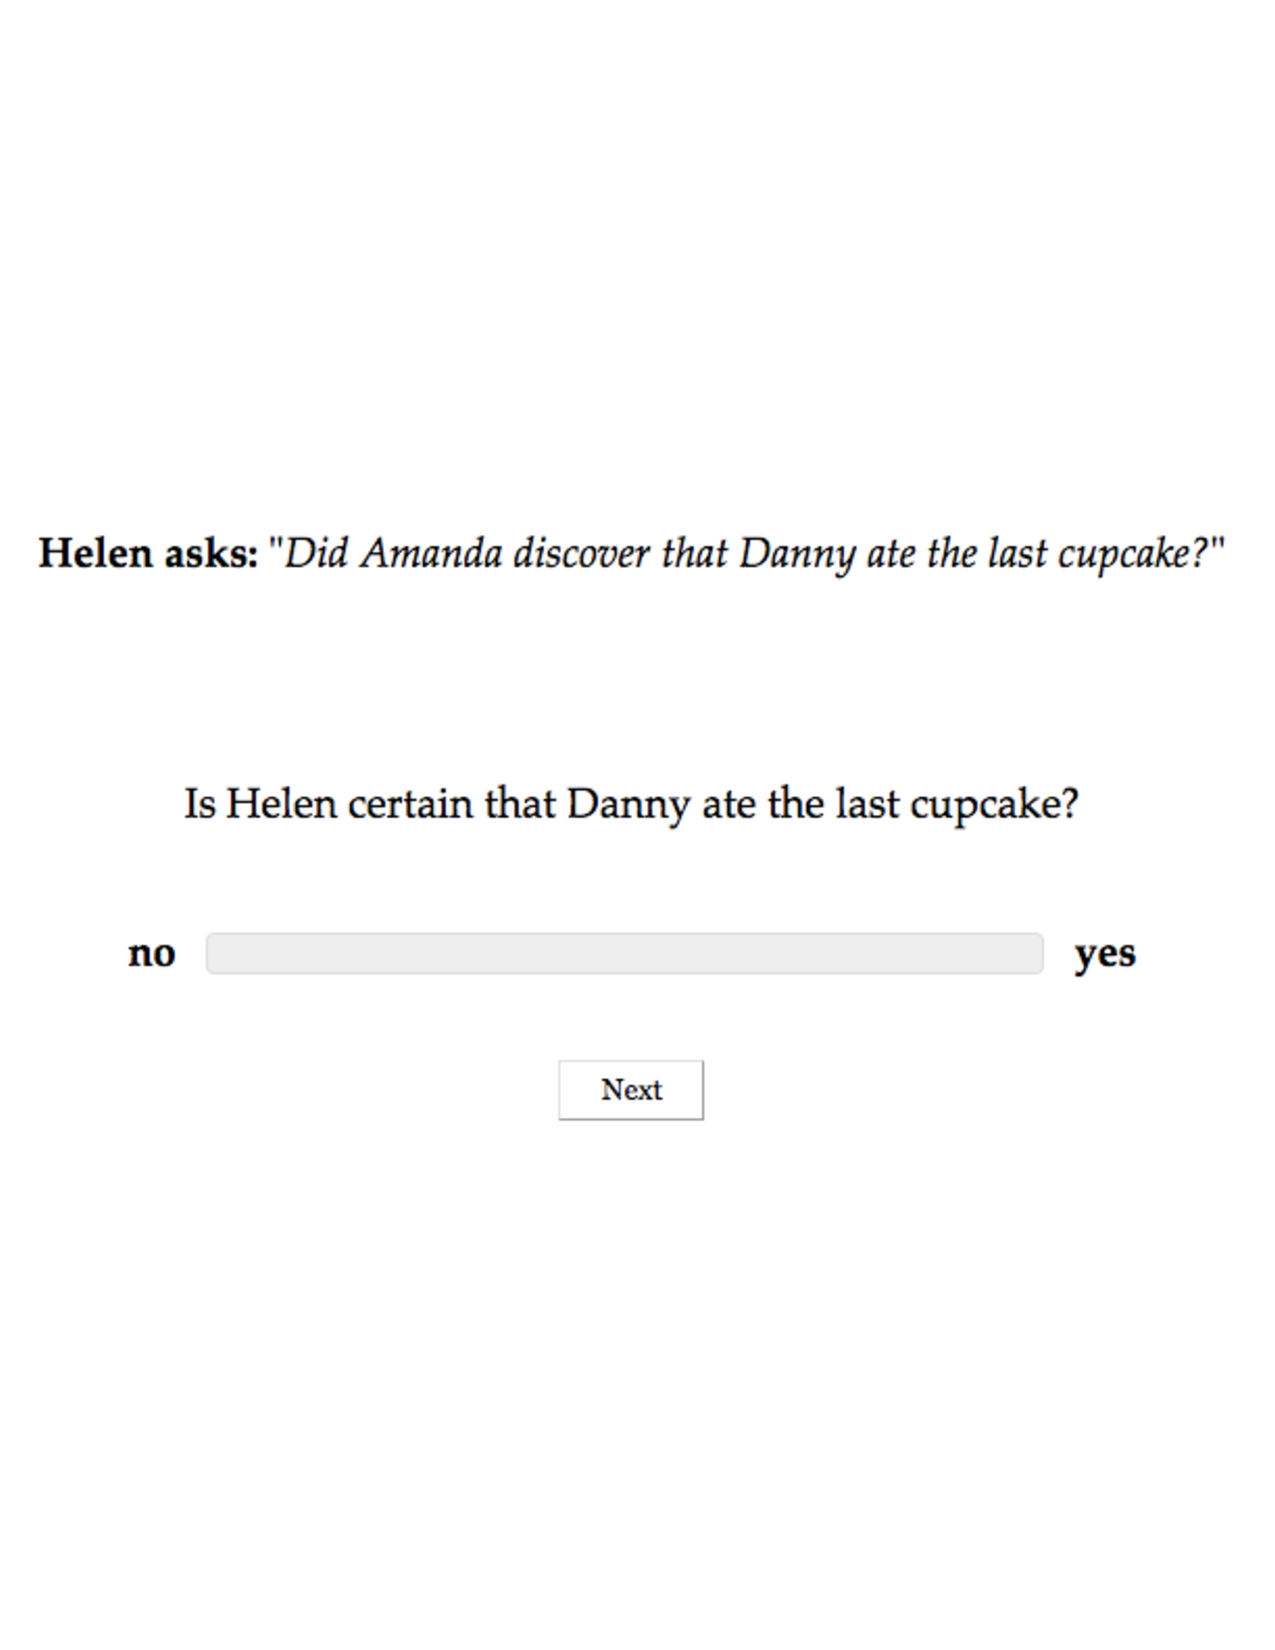
\includegraphics[width=10cm]{figures/trial-exp1}}
\end{center}
\caption{A sample trial in Experiment 1a}\label{fig-trial-exp1}
\end{figure}

%After completing the experiment (as well as the other five experiments we report on), participants filled out a short, optional survey about their age, their gender, their native language(s) and, if English is their native language, whether they are a speaker of American English (as opposed to, e.g., Australian or Indian English). To encourage them to respond truthfully, participants were told that they would be paid no matter what answers they gave in the survey.

\paragraph{Data exclusion} The data from 34 participants were excluded, based on self-declared non-native speaker status and other criteria given in Supplement \ref{a-excl}. The data from 266 participants (ages 20-71; median: 36; 118 female, 143 male, 2 other, 3 undeclared) were analyzed.

\subsubsection{Results and discussion}\label{s22}

Figure \ref{f-projectivity} shows the mean certainty ratings for the target stimuli by predicate as well as for the main clause stimuli (abbreviated `MC'), in increasing order from left to right. The mean certainty ratings were largely consistent with impressionistic judgments reported in the literature. First, the ratings for main clause content were lowest overall, as expected for non-projective content. Second, the ratings for factive predicates were among the highest overall, suggesting comparatively high projection of the CCs. Third, the mean certainty ratings of many optionally factive predicates were lower than those of many factive predicates and higher than those of main clauses as well as of non-veridical non-factives. However, Figure \ref{f-projectivity} also shows that the CCs of the 5 predicates assumed to be factive were not categorically more projective than the CCs of the optionally factive predicates, contrary to what is expected under the first definition of factive predicates. Specifically, the CCs of the optionally factive predicates {\em acknowledge, hear} and {\em inform} were at least as projective as the CCs of {\em reveal} or {\em discover}. \jt{This suggests that projection alone does not categorically distinguish factive predicates from optionally factive and non-factive ones.}

\begin{figure}[H]
\centering

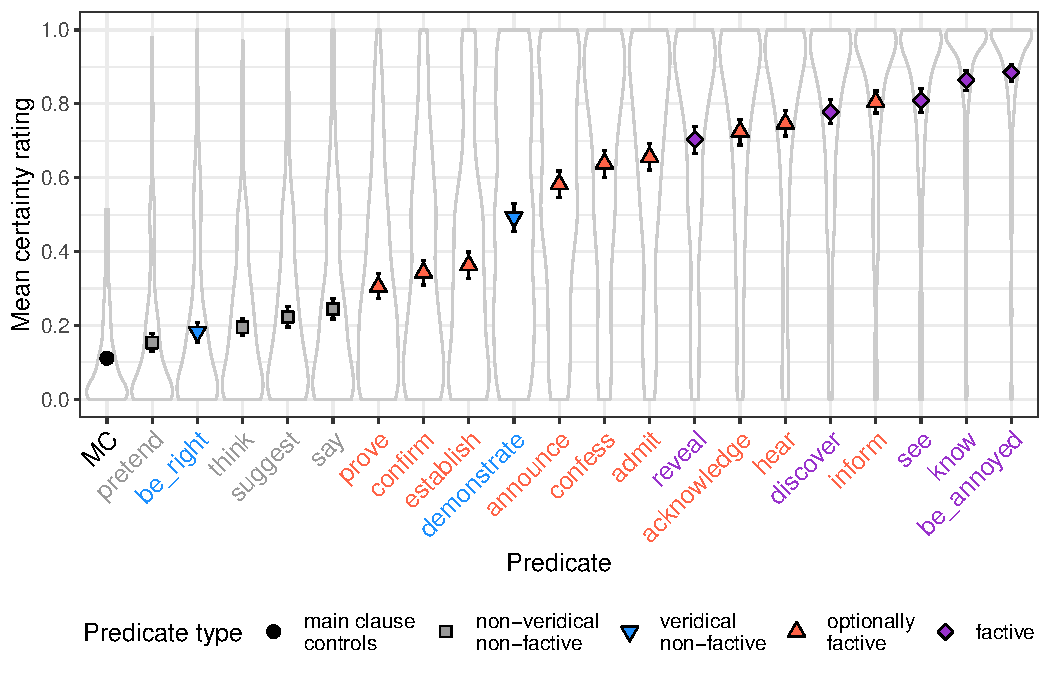
\includegraphics[width=.7\paperwidth]{../../results/5-projectivity-no-fact/graphs/means-projectivity-by-predicate-variability}

\caption{Mean certainty ratings by predicate in Exp.~1a. Error bars indicate 95\% bootstrapped confidence intervals. Light gray dots indicate individual participants' responses.} 
\label{f-projectivity}
\end{figure}




%1 acknowledge 0.725 0.0330  0.0339  0.692 0.758
% 2 admit       0.656 0.0390  0.0352  0.617 0.691
% 3 announce    0.582 0.0375  0.0370  0.545 0.619
% 4 be_annoyed  0.885 0.0220  0.0226  0.863 0.907
% 5 be_right    0.183 0.0271  0.0251  0.155 0.208
% 6 confess     0.639 0.0399  0.0376  0.599 0.676
% 7 confirm     0.343 0.0350  0.0358  0.308 0.379
% 8 MC          0.111 0.00895 0.00860 0.102 0.120
% 9 demonstrate 0.493 0.0403  0.0382  0.452 0.531
%10 discover    0.779 0.0303  0.0308  0.748 0.809
%11 establish   0.363 0.0340  0.0404  0.329 0.403
%12 hear        0.747 0.0371  0.0360  0.710 0.783
%13 inform      0.805 0.0287  0.0305  0.776 0.836
%14 know        0.864 0.0269  0.0241  0.837 0.888
%15 pretend     0.153 0.0232  0.0276  0.130 0.181
%16 prove       0.305 0.0314  0.0289  0.273 0.334
%17 reveal      0.704 0.0377  0.0349  0.666 0.739
%18 say         0.245 0.0283  0.0287  0.216 0.273
%19 see         0.809 0.0330  0.0303  0.776 0.840
%20 suggest     0.223 0.0256  0.0253  0.197 0.248
%21 think       0.195 0.0236  0.0243  0.172 0.220


In view of this result, one might ask whether the categorization of clause-embedding predicates assumed in (\ref{pred}) is correct: perhaps there is a different place in which a line can be drawn between factive predicates and others based on the projection of the CCs? The mean certainty ratings visualized in Figure \ref{f-projectivity} suggest that this cannot be done in a non-arbitrary way. For instance, one might consider all predicates factive whose CC is at least as projective as that of {\em reveal}. This would mean that the predicates typically taken to be factive are factive, as well as {\em acknowledge, hear} and {\em inform}. There is, however, no principled reason why the projection of the CC of {\em reveal} should be the cut-off for factivity. A different approach would be to pick an arbitrary mean certainty rating, say .8, and to categorize predicates whose CC has a mean certainty rating of at least .8 as factive and predicates whose CC has a mean certainty rating below .8 as optionally factive. However, this is as unprincipled an approach as the previous one---one could just as well pick a threshold of .85 or .75, with the result that different predicates would be considered factive. For instance, {\em discover} (mean: .78) would not count as factive with a threshold of .8, but would with a threshold of .75, and {\em see} (mean: .81) would count as factive with a threshold of .8, but not with a threshold of .85.\footnote{Choosing an arbitrary numeric threshold for factivity is also complicated by the fact that there is by-experiment variation in mean certainty ratings. For instance, the mean certainty ratings in Exp.~1a were lower, overall, than the mean certainty ratings in \citetpos{tbd-variability} Exps.~1. For example, the CC of {\em be annoyed}, which was the most projective in both sets of experiments, received mean certainty ratings of .96  and .92 in \citetpos{tbd-variability} Exps.~1a and 1b, respectively, but only a .86 in our Exp.~1a. This difference may be due to the fact that \citet{tbd-variability} primarily investigated highly projective content whereas our Exp.~1a included a wide range of less projective content: it is possible that participants' certainty ratings were influenced by the overall projection of the contents investigated.}

The possibility of categorizing clause-embedding predicates by the projection of the CC is further called into question by the fact that the CC of all of the 20 predicates investigated is projective, albeit to varying degrees, compared to the non-projective main clause controls. This was established by fitting a Bayesian mixed effects Beta regression model  with weakly informative priors using the \verb|brms| \citep{buerkner2017}  package in R \citep{R}. The model predicted the certainty ratings from a fixed effect of predicate (with treatment coding and `main clause control' as  reference level) and included the maximal random effects structure justified by the design, namely random by-participant and by-item intercepts. This random effects structure captures random variability in projection between participants and between items, where an item is a unique combination of a predicate and a complement clause. A Beta regression model estimates the mean of the outcome distribution (like a linear regression model).\footnote{Beta regression models also estimate a second parameter, namely the precision, which is a measure of dispersion: the greater the precision, the more concentrated the ratings are around the mean. In this paper, we rely on the estimated means to identify whether the CCs of the clause-embedding predicates differ from the relevant controls. Both the estimated mean and precision for each predicate are reported in the full model output tables in Supplement \ref{a-mo}.} We thus obtain, for each predicate, a 95\% credible interval for the mean rating for that predicate: this allows us to identify whether the mean ratings of the predicate and of the main clause controls differ. Supplement \ref{modeldetails} motivates the use of Beta regression over linear regression, provides a brief primer on how to interpret Bayesian mixed effects Beta regression models, and reports the full model output.

According to the Beta regression model, the estimated mean for each predicate was higher than that of the main clause controls, i.e., the 95\% credible intervals for the estimated adjustment to the main clause control mean did not contain 0 for any predicate. This result suggests that the CC of each of the 20 predicates is projective compared to non-projective main clause content, albeit to different degrees.\footnote{A Bayesian mixed effects linear regression with the same fixed and random effects structure yielded qualitatively identical results, except that the contrast between \emph{pretend} and the main clause controls was only marginally significant. See the Github repository mentioned in footnote \ref{f-github} for the model code.} Thus, to distinguish factive predicates from others in this set of 20 predicates, one would need to distinguish one group of  projective CCs from another group of projective CCs.

In sum, the results of Exp.~1a suggest that projection does not identify a coherent class of factive predicates. It is possible, however, that asking participants to assess projection with a gradient response scale encouraged them to provide non-categorical answers and that the observed projection variability is an artifact of the task. If so, categorically distinguishing factive predicates from others may be possible if participants were asked to assess projection with a categorical response task. To assess this possibility, we conducted Exp.~1b, which was identical to Exp.~1a but employed a two-alternative forced choice task.


\subsection{Experiment 1b: Categorical projection ratings}\label{s-exp1b}

\subsubsection{Methods}

\paragraph{Participants} 600 participants with U.S.\ IP addresses and at least 99\% of previous HITs approved were recruited on Amazon's Mechanical Turk platform. They were paid \$1.\footnote{Exps.~1a, 2a and 3a were run in 2017 and 2018, whereas  Exps.~1b, 2b and 3b were run in 2019. Participants in the later experiments were paid more to reflect an increased minimum wage in $[$the region in which the researchers ran the experiment$]$.}


\paragraph{Materials and procedure} The materials and procedure were identical to those of Exp.~1a, with the exception of the task: participants responded `yes' (coded as 1) or `no' (coded as 0) to the question of whether the speaker is certain of the relevant content, as shown in Figure \ref{fig-trial-exp1b}.

\begin{figure}[h!]
\begin{center}
\fbox{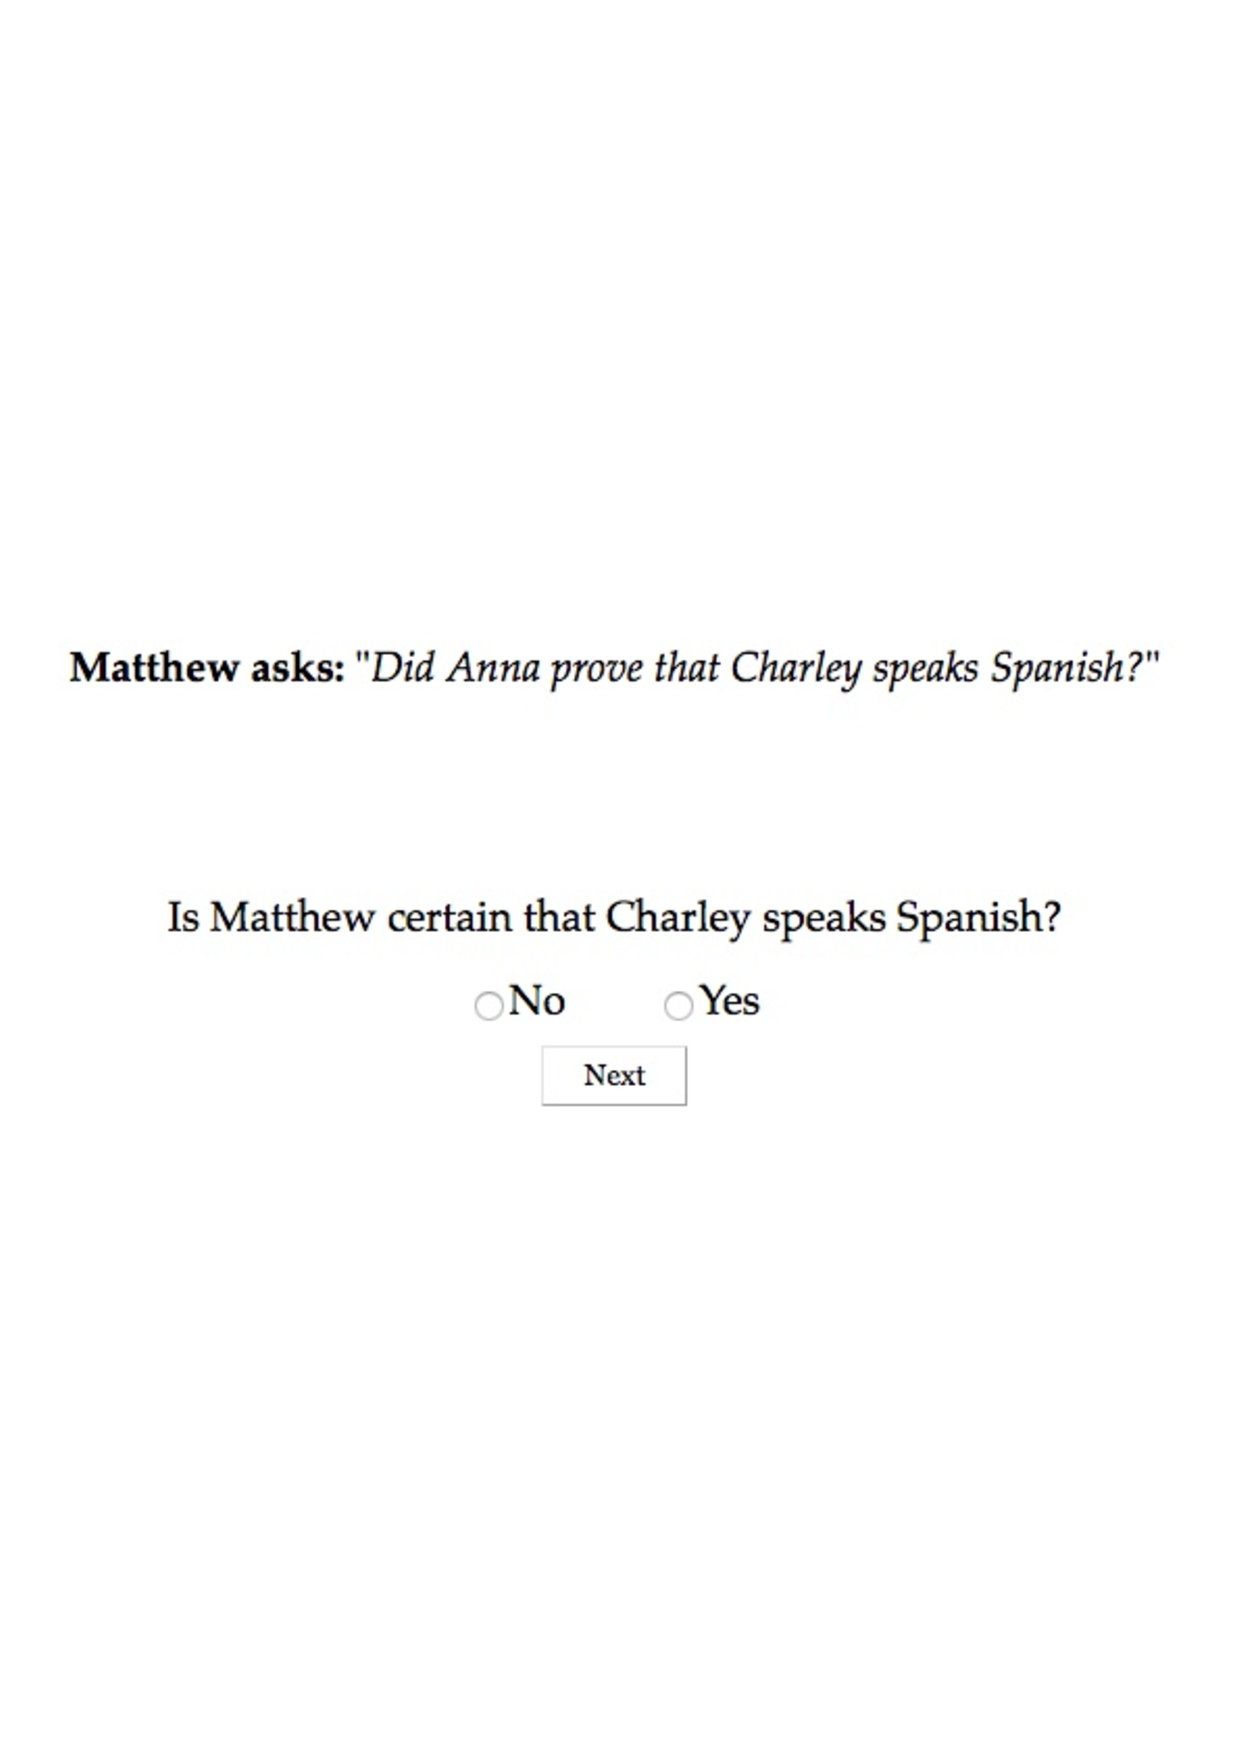
\includegraphics[width=10cm]{figures/Exp1b-trial}}
\end{center}
\caption{A sample trial in Experiment 1b}\label{fig-trial-exp1b}
\end{figure}

\paragraph{Data exclusion} The data from 164 participants were excluded according to the criteria given in Supplement \ref{a-excl}. The data from 436 participants (ages 18-81; median: 37; 207 female, 223 male, 2 other) were analyzed.

\subsubsection{Results and discussion}

Figure \ref{f-projectivity2} shows the proportion of `yes' ratings (indicating projection) for the predicates and the main clause stimuli, in increasing order from left to right. Jittered gray dots indicate the individual participants' ratings.\footnote{Recall that participants gave binary certainty ratings, with `yes' coded as 1 and `no' coded as 0. To increase legibility, these ratings are jittered vertically in Figure \ref{f-projectivity2} and other figures like it. Consequently, the individual certainty ratings should not be read against the y-axis.} The order of predicates according to the projection of their CC in Exp.~1b is strikingly similar to that of Exp.~1a, as evidenced by the very high Spearman rank correlation of .983 (see Supplement \ref{a-comparison} for a visualization and details on this correlation). The critical results of Exp.~1a were replicated. First, the CCs of the factive predicates were not categorically more projective than the CCs of the optionally factive predicates:  the CCs of {\em acknowledge, hear} and {\em inform} were again at least as projective as the CCs of {\em reveal} or {\em discover}. Second, a non-arbitrary line between factive and optionally factive predicates cannot be drawn: the CCs of all 20 predicates were projective compared to the non-projective main clause controls.\footnote{According to \citet[1739]{spector-egre2015}, it is not clear whether the CC of {\em say} is projective. The results of our Exps.~1 suggest that it is weakly projective.}  This was established by fitting a Bayesian mixed effects logistic regression model  with weakly informative priors using the \verb|brms| package in R. The model predicted the log odds of a `yes' over a `no' response from a fixed effect of predicate (with treatment coding and `main clause' as  reference level) and included the maximal random effects structure justified by the design, namely random by-participant and by-item intercepts. The estimated log odds of a `yes' response was greater for each predicate than that of the main clause controls, i.e., the 95\% credible intervals for the estimated coefficients did not contain 0 for any predicate. See Supplement \ref{a-mo} for model details. Thus, like Exp.~1a, the results of Exp.~1b \jt{do not support the assumption of the definition of factive predicates in (\ref{def}a) that factive predicates are categorically distinguished from optionally factive and non-factive ones by the projection of the CC.}

\begin{figure}[H]

\centering
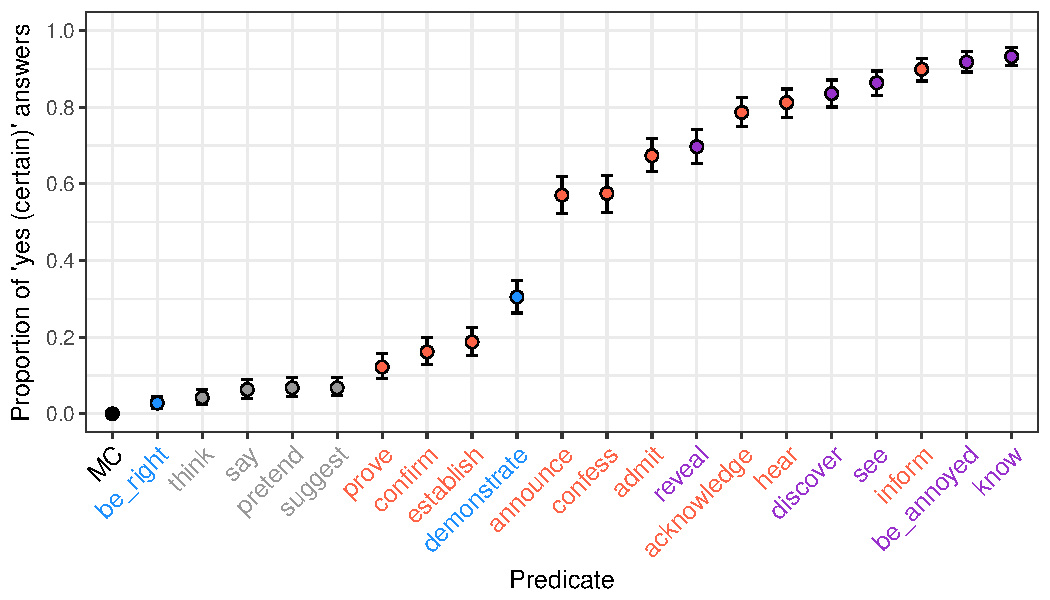
\includegraphics[width=.7\paperwidth]{../../results/8-projectivity-no-fact-binary/graphs/proportion-by-predicate-variability}
\caption{Proportion of `yes' ratings by predicate in Exp.~1b. Error bars indicate 95\% bootstrapped confidence intervals. Gray dots indicate individual participant responses (either 0 or 1, jittered vertically for legibility).}
\label{f-projectivity2}

\end{figure}

\subsection{Interim summary and alternative analyses}
\label{sec:interimproj}

The results of Exps.~1 suggest that \jt{projection does not categorically distinguish factive predicates from others.} We observed, contrary to what is expected on definition (\ref{def}a), that the CCs of predicates standardly classified as factive are not categorically more projective than the CCs of all other predicates. 

One objection to this conclusion is that the expectation that the CCs of factive predicates should be more projective than those of all other predicates is too strong. Specifically, given that the CCs of factive predicates are among the most projective in both Exps.~1a and 1b, one might argue that to motivate a class of factive predicates it suffices to show that assuming such a class explains  variability observed in the projection of the CCs of clause-embedding predicates. To engage with this possibility, we analyzed the certainty ratings of Exps.~1 in a Bayesian mixed effects Beta regression model (Exp.~1a) and a logistic regression model (Exp.~1b) that predicted projection from a binary factivity predictor, whereby the five predicates in (\ref{pred}a) were classified as factive and the remaining predicates (as well as the main clause controls) as non-factive. We report mean estimates and 95\% credible intervals for the effect of this binary factivity predictor. Under such an analysis of the predicates, the CCs of presumed factive predicates were indeed more projective, both in Exp.~1a ($\beta = 1.49, CI = [1.30, 1.67]$) and in Exp.~1b ($\beta = 3.99, CI = [3.40,4.59]$). It may thus be tempting to conclude that projection-based factivity is a useful category to maintain.

% ternary factivity predictor logit model: opt-factive ($\beta = 3.73, CI = [3.22,4.24]$)) and factive ($\beta = 6.61, CI = [6.01,7.19]$))

There are two reasons not to do so. The first is that, as already observed in sections  \ref{s-exp1a} and \ref{s-exp1b}, there is no clear threshold that divides the presumed factive predicates from the others. That is, while the CCs of presumed factive predicates are \emph{on average} more projective than those of other predicates, they are not more projective in comparison with each individual predicate.  Some readers may not be troubled by this and entertain the possibility that factivity is a fuzzy category rather than one with clear boundaries. We discuss this possibility further in section \ref{s4}.

The second reason not to maintain the category is that the binary factivity models capture less of the variability than the models that include the individual predicates as predictors, which were reported in sections \ref{s-exp1a} and \ref{s-exp1b}. We refer to these latter models as predicate-specific models. Model comparison revealed that predicate-specific models were favored over binary factivity models in both Exp.~1a (WAIC of predicate-specific model: -18971.3 (SE= 359.3); WAIC of binary factivity model: -18643.9 (SE= 355.4))  and Exp.~1b (WAIC of predicate-specific model: 6444.5 (SE= 124.8); WAIC of binary factivity model: 6719.0 (SE= 123.7)).\footnote{The Widely Applicable Information Criterion (WAIC) is a measure of model quality that estimates the pointwise out-of-sample prediction accuracy from a fitted Bayesian model using the log-likelihood evaluated at the posterior simulations of the parameter values and penalizes models with more parameters over models with fewer \citep{watanabe2010}. We obtained WAIC values for each model using the \texttt{loo} package \citep{vehtari2017}. Lower WAIC values indicate better models.} This suggests that the qualitative observation made in sections  \ref{s-exp1a} and \ref{s-exp1b}, namely that projection variability is better captured by taking into account the individual predicates than a binary factivity classification, is borne out in rigorous model comparison. 

% ternary waic beta model: 
% ternary waic logit model: 6711.3 (SE=124.5)


\subsection{Converging evidence for failure of projection-based definition of factive predicates}\label{s-converging1}

The results of  Exps.~1a and 1b suggest that the definition of factive predicates in (\ref{def}a), according to which a predicate is factive if and only if its CC is presupposed, \jt{fails to identify a class of factive predicates.} We now discuss converging evidence to this effect from three additional datasets: the CommitmentBank (\citealt*{demarneffe-etal-sub23}), the MegaVeridicality dataset (\citealt{white-rawlins-nels2018,white-etal2018b}) and the VerbVeridicality dataset (\citealt{ross-pavlick2019}).\footnote{We re-plotted the data, obtained at \url{https://github.com/mcdm/CommitmentBank}, \url{http://megaattitude.io} and \url{https://github.com/alexisjihyeross/verb_veridicality}, respectively. For the analysis files, see the GitHub repository mentioned in footnote \ref{f-github}.}

The CommitmentBank is a collection of 1,200 naturally occurring English discourses from the Wall Street Journal, the British National Corpus and the Switchboard corpus: each discourse consists of a target sentence with a clause-embedding predicate embedded an entailment-canceling operator and up to two preceding context sentences, as illustrated in (\ref{cb}), with {\em know} in the target sentence embedded under negation:

\begin{exe}
\ex\label{cb} What fun to hear Artemis laugh. She's such a serious child. I didn't know she had a sense of humor. \\ \hspace*{.2cm} \hfill (\citealt[109]{demarneffe-etal-sub23})
\end{exe}
Annotators recruited on Amazon's Mechanical Turk platform provided certainty ratings for the CCs of the target sentences on a 7-point Likert scale labeled at three points: speaker/author is certain that the CC is true (coded as 3), speaker/author is not certain whether the CC is true or false (coded as 0), and speaker/author is certain that the CC is false (coded as -3); the lower half of the scale was included to differentiate speaker/author non-commitment to the CC from speaker/author commitment to the falsity of the CC (as may arise in, for instance, {\em I don't know that I agree.}). \citet{demarneffe-etal-sub23} assumed, for certainty ratings above 0, that the higher the certainty rating, the more projective the CC. Figure \ref{f-commitmentbank} shows the mean certainty ratings for the CCs in the 982 discourses with 45 non-veridical non-factive, optionally factive and factive clause-embedding predicates (target sentences embedded under non-epistemic modals were excluded; see \citealt[\S3]{demarneffe-etal-sub23}). In line with the results of Exps.~1, projection of the CC does not categorically distinguish factive predicates from optionally factive and non-factive ones: for instance, the CCs of the optionally factive predicates {\em foresee, confess, show, tell} and {\em accept} are at least as projective as those of some factive predicates.\footnote{\citealt{demarneffe-etal-sub23} found that a model that predicts certainty ratings from factivity captures less of the variance than a model that predicts certainty ratings from predicate lemma. This result is replicated in our Exps.~1, as discussed above.}

\begin{figure}[H]
\centering
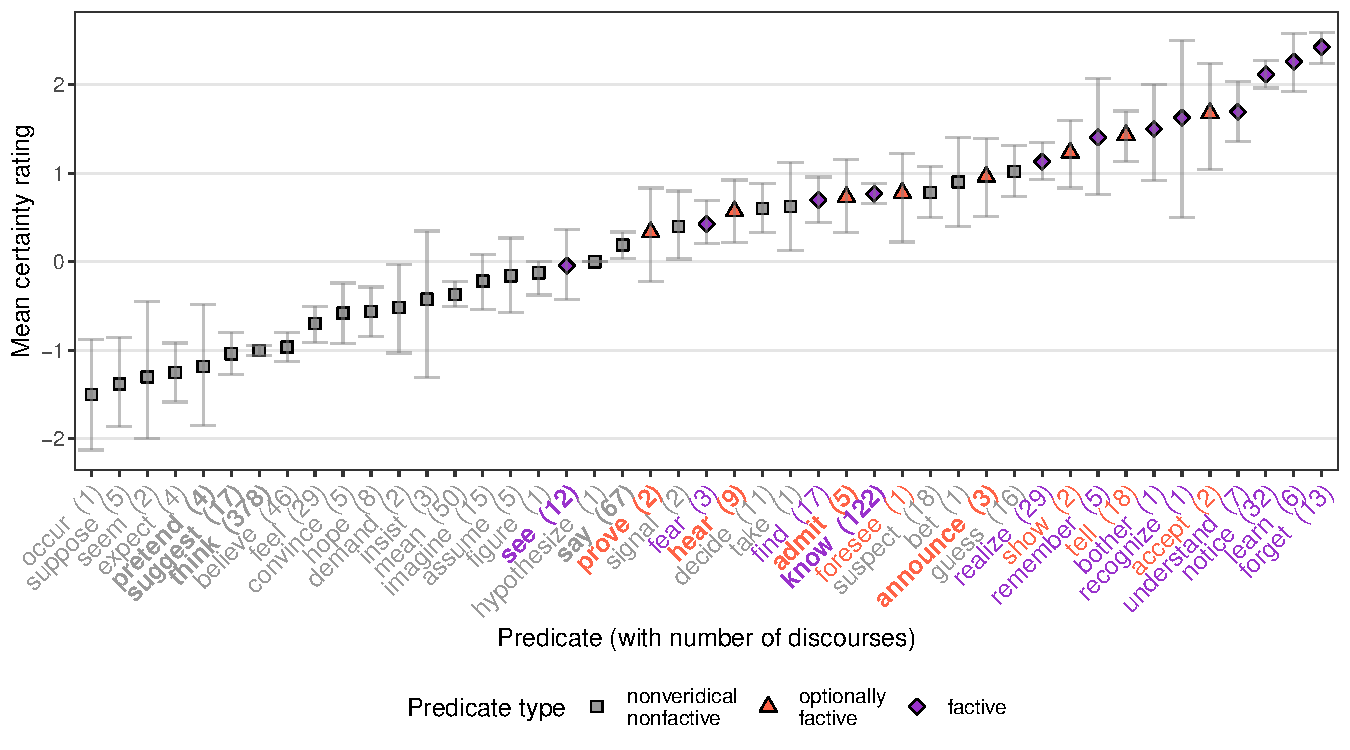
\includegraphics[width=.75\paperwidth]{../../CommitmentBank-analysis/graphs/means-projectivity-by-predicate-variability}

\caption{Mean certainty ratings by predicate, with number of discourses in parentheses, for 982 discourses in the CommitmentBank (\citealt*{demarneffe-etal-sub23}). Error bars indicate 95\% bootstrapped confidence intervals. Predicates included in our Exps.~1 shown in bold.}
\label{f-commitmentbank}
\end{figure}

A second piece of converging evidence that the definition in (\ref{def}a) fails to identify a class of factive predicates comes from the VerbVeridicality dataset. This dataset includes 859 naturally occurring indicative matrix sentences with a total of 78 clause-embedding predicates and their clausal complements from the MultiNLI (\citealt{williams-etal2018}) corpus. To diagnose projection of the CC, negated variants of the 859 matrix sentences were created; an example is given in (\ref{vv-stim-proj}). For each negated variant, three participants rated on a 5-point Likert scale whether the CC is true given the target sentence; one endpoint of the scale was labeled `definitely true' (coded as 2) and the other `definitely not true' (coded as -2).
%\footnote{\citealt{ross-pavlick2019} investigated the extent to which the CCs follow from the indicative matrix sentences and from their negated counterparts. While they refer to both as `veridicality' inferences, the latter is typically called `projection' in the semantics/pragmatics literature.}

\begin{exe}
\ex\label{vv-stim-proj} The GAO has not indicated that it is unwilling to compromise. \hfill (\citealt[2234]{ross-pavlick2019})
\end{exe}

Figure \ref{f-vv-projectivity} plots the mean projection ratings for the CCs of the 78 predicates in the VerbVeridicality dataset, with labels for the 15 predicates from our Exps.~1 that are included ({\em see} and {\em saw}, which are both included in the VerbVeridicality dataset, are plotted separately). As shown, projection does not categorically distinguish factive predicates from optionally factive and non-factive ones: the CCs of all of our optionally factive predicates are at least as projective as that of some factive predicate. 

\begin{figure}[H]
\centering
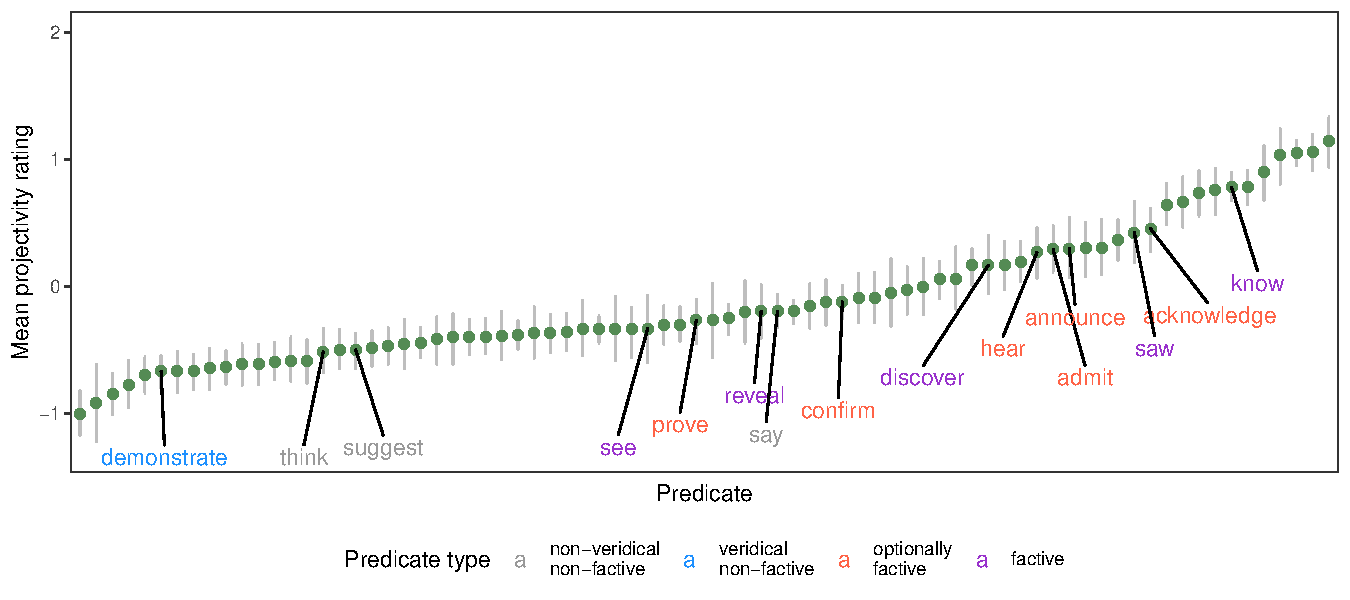
\includegraphics[width=.77\paperwidth]{../../VerbVeridicality-analysis/graphs/means-projection-by-predicate}

\caption{Mean projection rating by predicate in green, with 95\% bootstrapped confidence intervals, for the 78 predicates in the VerbVeridicality dataset (\citealt{ross-pavlick2019}), with labels for the 15 predicates featured in our experiments.}
\label{f-vv-projectivity}
\end{figure}



A third piece of converging evidence comes from the MegaVeridicality dataset, which contains projection ratings for the CCs of 517 English clause-embedding predicates. The stimuli that participants rated consisted of combinations of these predicates with what \citet{white-rawlins-nels2018} referred to as low content arguments, as shown in (\ref{wr-stim-proj}) for {\em know}. The predicates were embedded under negation in stimuli like (\ref{wr-stim-proj}a) and under negation, in the antecedent of a conditional and in a question in stimuli like (\ref{wr-stim-proj}b). To assess projection, participants were asked to respond to the question {\em Did that thing happen?} for stimuli like (\ref{wr-stim-proj}a) and to respond to the question posed by stimuli like (\ref{wr-stim-proj}b). The response options were `yes', `maybe or maybe not' and `no'. 

\begin{exe}
\ex\label{wr-stim-proj}
\begin{xlist}
\ex Somebody didn't know that a particular thing happened.
\ex If somebody didn't know that a particular thing happened, did that thing happen?
\end{xlist}
\end{exe}

The CCs of each of the 517 predicates in the MegaVeridicality dataset received between 29 and 60 projection ratings (mean: 32). To plot the ratings, we coded a `yes' response as 1 (the speaker is certain that the thing happened),  a `maybe or maybe not' response as 0 (the speaker is not certain whether the thing happened) and a `no' response as -1 (the speaker is certain that the thing didn't happen). Figure \ref{f-white-rawlins-projectivity} plots the mean projection ratings for the 517 predicates in the MegaVeridicality dataset, with labels for the 19 predicates from our experiments that are included. As shown, projection of the CC does not categorically distinguish factive predicates from others: for instance, the CCs of the optionally factive predicates {\em confess, acknowledge, admit, announce, hear} and {\em inform} are at least as projective as those of some factive predicates. 

\begin{figure}[H]
\centering
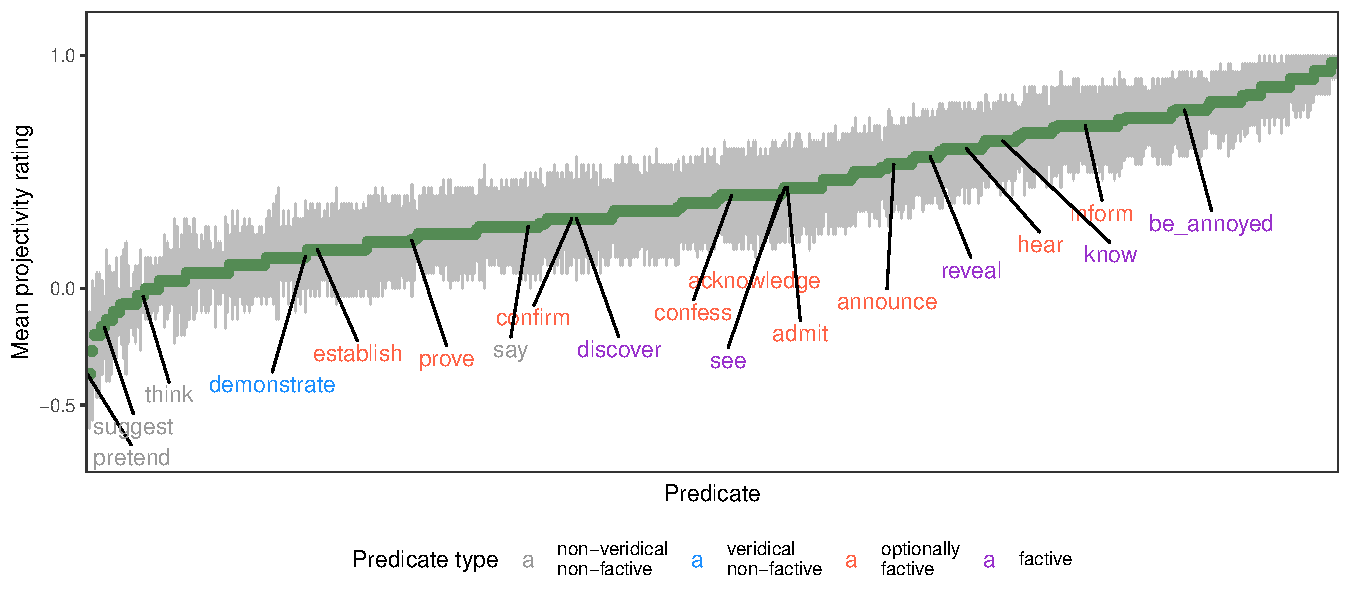
\includegraphics[width=.77\paperwidth]{../../MegaVeridicality-analysis/graphs/means-projection-by-predicate}

\caption{Mean projection rating by predicate in green, with 95\% bootstrapped confidence intervals, for the 517 predicates in the MegaVeridicality dataset (\citealt{white-rawlins-nels2018,white-etal2018b}), with labels for the 19 predicates featured in our experiments.}
\label{f-white-rawlins-projectivity}
\end{figure}


In sum, contrary to what is expected under the definition of factive predicates in (\ref{def}a), the results of our Exps.~1a and 1b as well as those of the CommitmentBank, the VerbVeridicality dataset, and the MegaVeridicality dataset suggest that projection of the CC \jt{fails to identify a coherent class of factive predicates.} The challenge to definition (\ref{def}a) is compounded by the diversity of the empirical evidence: it comes from constructed and naturally occurring examples, from examples presented with and without a context, from examples with diverse and with minimal lexical content, from clause-embedding predicates embedded under different entailment-canceling operators, and from projection ratings collected through different response tasks. 

The experiments described in the next section were designed to explore whether the definition of factive predicates in (\ref{def}b), according to which presupposition and entailment jointly identify a class of factive predicates, is empirically supported. To this end, we collected entailment judgments for CCs of the same 20 predicates studied in Exps.~1.

\section{Experiments 2 and 3: Entailment}\label{s3}

Experiments 2 and 3 explored which of the CCs of the 20 clause-embedding predicates are entailed, to identify whether the definition of factive predicates in (\ref{def}b) identifies a coherent class of factive predicates. We assume the standard definition of entailment, according to which entailment is a binary, categorical relation between two contents: given sentences $\phi$ and $\psi$, the content of $\phi$ entails the content of $\psi$ if and only if every world in which $\phi$ is true is also a world in which $\psi$ is true. If there is at least one world in which $\phi$ is true but $\psi$ is false, then $\phi$ does not entail $\psi$. 

To establish whether the content of an indicative matrix sentence with a clause-embedding predicate entails the CC, we used two standard diagnostics for entailment, given in (\ref{diag}). According to the `inference diagnostic' in (\ref{diag}a), the content of an indicative matrix sentence with a clause-embedding predicate entails the CC if and only if the CC definitely follows from a true statement of the matrix sentence. According to the `contradictoriness diagnostic' in (\ref{diag}b), an entailment relationship holds if and only if an utterance of the indicative matrix sentence that is followed by a denial of the CC is contradictory. 

\begin{exe}
\ex\label{diag} Two diagnostics for entailment \hfill (see, e.g., \citealt[\S3.1]{ccmg90})
\begin{xlist}
\ex  Inference diagnostic (Exps.~2a and 2b)\\ $\phi$ entails $\psi$ if and only if, if $\phi$ is true, then the truth of $\psi$ definitely follows. 

\ex  Contradictoriness diagnostic  (Exps.~3a and 3b)\\ $\phi$ entails $\psi$ if and only if a sentence of the form {\em $\phi$ and not $\psi$} is contradictory. 

\end{xlist}
\end{exe}
These two diagnostics for entailment were applied to the CCs of the 20 clause-embedding predicates in Exps.~2a/2b and Exps.~3a/3b, respectively: the two versions of each experiment differed in whether participants provided a gradient response (a) or a categorical one (b).  Both sets of experiments included control stimuli for which the relevant contents stand in an entailment relation, that is, for which the relevant inference definitely follows (Exps.~2) and that are definitely contradictory (Exps.~3). We assume that the CC of a clause-embedding predicate is not entailed if responses to the CC are significantly different from responses to these control stimuli and that the CC of a clause-embedding predicate is entailed if responses to the CC are not significantly different from responses to these control stimuli. Thus, identifying entailed CCs  requires arguing from a null result. Given the standard classification of the 20 clause-embedding predicates in (\ref{pred}), we expect the CCs of factive and veridical non-factive predicates to be entailed, i.e., to not be judged   differently from the control stimuli.

%Given this definition, establishing that the contents of two natural language sentences $\phi$ and $\psi$ do not stand in an entailment relation involves identifying a world in which the content of $\phi$ is true and the content of $\psi$ is false. 

%\jd{the following sentence is rhetorically a little weird: aren't we precisely interested in identifying when there \emph{is} an entailment relationship? the way it's framed makes it sound liike we're mostly interested in showing non-entailment.---more generally, do we need all the detail of this paragraph or can we just move directly to the next paragraph, which introduces the standard diagnostics for entailment?} In this paper, however, we are also interested in establishing that the contents of two sentences $\phi$ and $\psi$  do stand in an entailment relation. Establishing this is straightforward if the content of some expression in $\phi$ denotes a subset of the content of some expression in $\psi$: for instance, in (\ref{ent1}a),  the content of $\phi$ entails the content of $\psi$ because the denotation of {\em black cat} in $\phi$ is a subset of the denotation of {\em cat} in $\psi$. No such structural relation exists, however, between the content of a sentence with a clause-embedding predicate and the CC, as in (\ref{ent1}b). %Furthermore, it is of course impossible to empirically verify that the content of $\phi$ entails the content of $\psi$ in (\ref{ent1}b) because it is impossible to verify that $\psi$ is true in all worlds in which $\phi$ is true. 
%
%\begin{exe}
%\ex\label{ent1}
%\begin{xlist}
%\ex $\phi$: Sam owns a black cat. \hspace*{1.5cm} $\psi$: Sam owns a cat.
%
%\ex $\phi$: Sam knows that it's raining. \hspace*{.6cm} $\psi$: It's raining.
%
%\end{xlist}
%\end{exe}

%\footnote{\citealt{sudo-thesis} proposed to diagnose whether a presupposition is an entailment based on whether the presupposition obligatorily restrict the domain of the quantifier {\em exactly one}. According to this diagnostic, the pre-state content of {\em stop} is a presupposition and an entailment because (ia) means that exactly one student who used Mac stopped using Mac. On the other hand, the gender presupposition of {\em she} in (ib) is not an entailment because (ib) does not mean that exactly one female student criticized herself, but that exactly one student criticized herself (see \citealt{zehr-schwarz2016,zehr-schwarz2018} for some experimental support). According to this diagnostic, the CC of {\em know} is entailed content: (ic) means that exactly one student who got accepted by MIT knows that they got accepted by MIT. {\bf REVISE THIS: Whether the {\em exactly one} diagnostic can help settle the debate about which contents of complements of clause-embedding predicates are entailed is a question we leave for future research.}
%
%\begin{exe}
%\exi{(i)} 
%\begin{xlist}
%\ex Exactly one student stopped using Mac. \hfill (\citealt[59]{sudo-thesis})
%
%\ex Exactly one student criticized herself. \hfill (\citealt[61]{sudo-thesis})
%
%\ex Exactly one student knows that they got accepted by MIT. \hfill (\citealt[64]{sudo-thesis})
%
%\end{xlist}
%\end{exe}}

\subsection{Exp.~2a: Gradient ratings using the inference diagnostic for entailment}\label{s31}

Exp.~2a investigated which of the CCs of the 20 clause-embedding predicates are entailed based on the inference diagnostic for entailment in (\ref{diag}a). Participants assessed on a gradient scale whether the CC follows from true statements of indicative matrix sentences with the 20 clause-embedding predicates.

%In contrast to the entailment relationship, which is categorical and categorical, the inference relationship is gradient: given true statements $\phi_1$ and $\phi_2$, the inference to the truth of $\psi$ may be stronger from $\phi_1$ than from $\phi_2$. To illustrate assume that $\phi_1$ is the sentence {\em Julian is from Cuba} and that $\phi_2$ is the sentence {\em Julian is from Germany}: the inference to the truth of $\psi$ {\em Julian dances salsa} is stronger from $\phi_1$ than from $\phi_2$.

% To illustrate, assume that Chris wears his pajamas when he is at home and that he doesn't wear pajamas outside of his home. Now consider the sentences $\phi_1$ to $\phi_5$ in (\ref{chris}). Given the aforementioned assumption, the truth of the content of the statement $\psi$ {\em Chris is wearing his pajamas} definitely follows from a true statement of $\phi_1$\jd{is this true?---the way the assumption is formulated above, it's a habitual---ie, he habitually wears pajamas at home and not outside the home; but presumably, there is a point in time at which he changes from pajamas to outside clothes, so he doesn't wear just pajamas at home, so it doesn't follow from $\phi_5$ that Chris is wearing pajamas}, it follows to increasingly lower degrees from true statements of $\phi_2$ to $\phi_4$ and it does not follow from a true statement of $\phi_5$. 
%
%\begin{exe}
%\ex\label{chris}
%\begin{xlist}
%\exi{$\phi_1$} Chris is at home.
%\exi{$\phi_2$} Chris is likely at home.
%\exi{$\phi_3$} Chris is possibly at home.
%\exi{$\phi_4$} There is a slight possibility that Chris is at home.
%\exi{$\phi_5$} Chris is not at home.
%\end{xlist}
%\end{exe}

\subsubsection{Methods}

\paragraph{Participants} 300 participants with U.S.\ IP addresses and at least 99\% of previous HITs approved were recruited on Amazon's Mechanical Turk platform (ages: 19-69, median: 36; 152 female, 148 male). They were paid \$0.75.

\paragraph{Materials} The target stimuli were 400 indicative matrix sentences. They were constructed by combining the 20 clause-embedding predicates with the 20 complement clauses (for 400 predicate/clause combinations, as in Exps.~1) and a proper name subject whose gender differed from the gender of the proper name subject of the embedded clause. As illustrated in the sample stimuli in (\ref{stims2}), these matrix sentences were presented to participants as true statements. For each of the 400 target stimuli, the inference that was tested was the inference to the CC: for instance, participants were asked about (\ref{stims2}a) whether it follows that Danny ate the last cupcake and about (\ref{stims2}b) whether it follows that Emma studied on Saturday morning.

\begin{exe}
\ex\label{stims2}
\begin{xlist}
\ex {\bf What is true:} Melissa knows that Danny ate the last cupcake.
\ex {\bf What is true:} Jerry pretended that Emma studied on Saturday morning.
\end{xlist}
\end{exe}

The experiment included eight control stimuli that were used to assess whether participants were attending to the task and interpreted the task correctly, as well as to identify inference ratings for entailed content. There were four entailing control stimuli for which the tested inferences are entailments of the true statements: in the sample entailing control in (\ref{control-good2}), for instance, that Frederick solved the problem is an entailment of the true statement that Frederick managed to solve the problem. We expected the inference ratings for these four control stimuli to be at ceiling and, as discussed above, we rely on the ratings for these stimuli to identify entailments. In contrast, the inferences tested with the four non-entailing control stimuli, like (\ref{control-bad2}), definitely do not follow from these true statements: for instance, in (\ref{control-bad2}), that Dana wears a wig does not follow from Dana watching a movie last night. We expected the inference ratings for these four control stimuli to be at floor. See Supplement \ref{a-control} for the full set of control stimuli.

\begin{exe}
\ex\label{control-good2} {\bf What is true:} Frederick managed to solve the problem. (Tested inference: Frederick solved the problem.)
\ex\label{control-bad2}  {\bf What is true:} Dana watched a movie last night. (Tested inference: Dana wears a wig.)
\end{exe}

Each participant saw a random set of 28 stimuli: each set contained one target stimulus for each of the 20 predicates (each with a unique complement clause) and the same 8 control stimuli. Trial order was randomized.

\paragraph{Procedure} Participants were told that they would read true statements and that they would be asked to assess whether a second statement follows from that true statement. On each trial, participants read the true statement and were asked to respond to the question {\em Does it follow that\ldots?}, with the complement clause realized by the complement clause of the clause-embedding predicate. Participants responded on a sliding scale from `definitely doesn't follow' (coded as 0) to `definitely follows' (coded as 1), as shown in Figure \ref{f-trial-exp3}.

\begin{figure}[H]
\begin{center}
\fbox{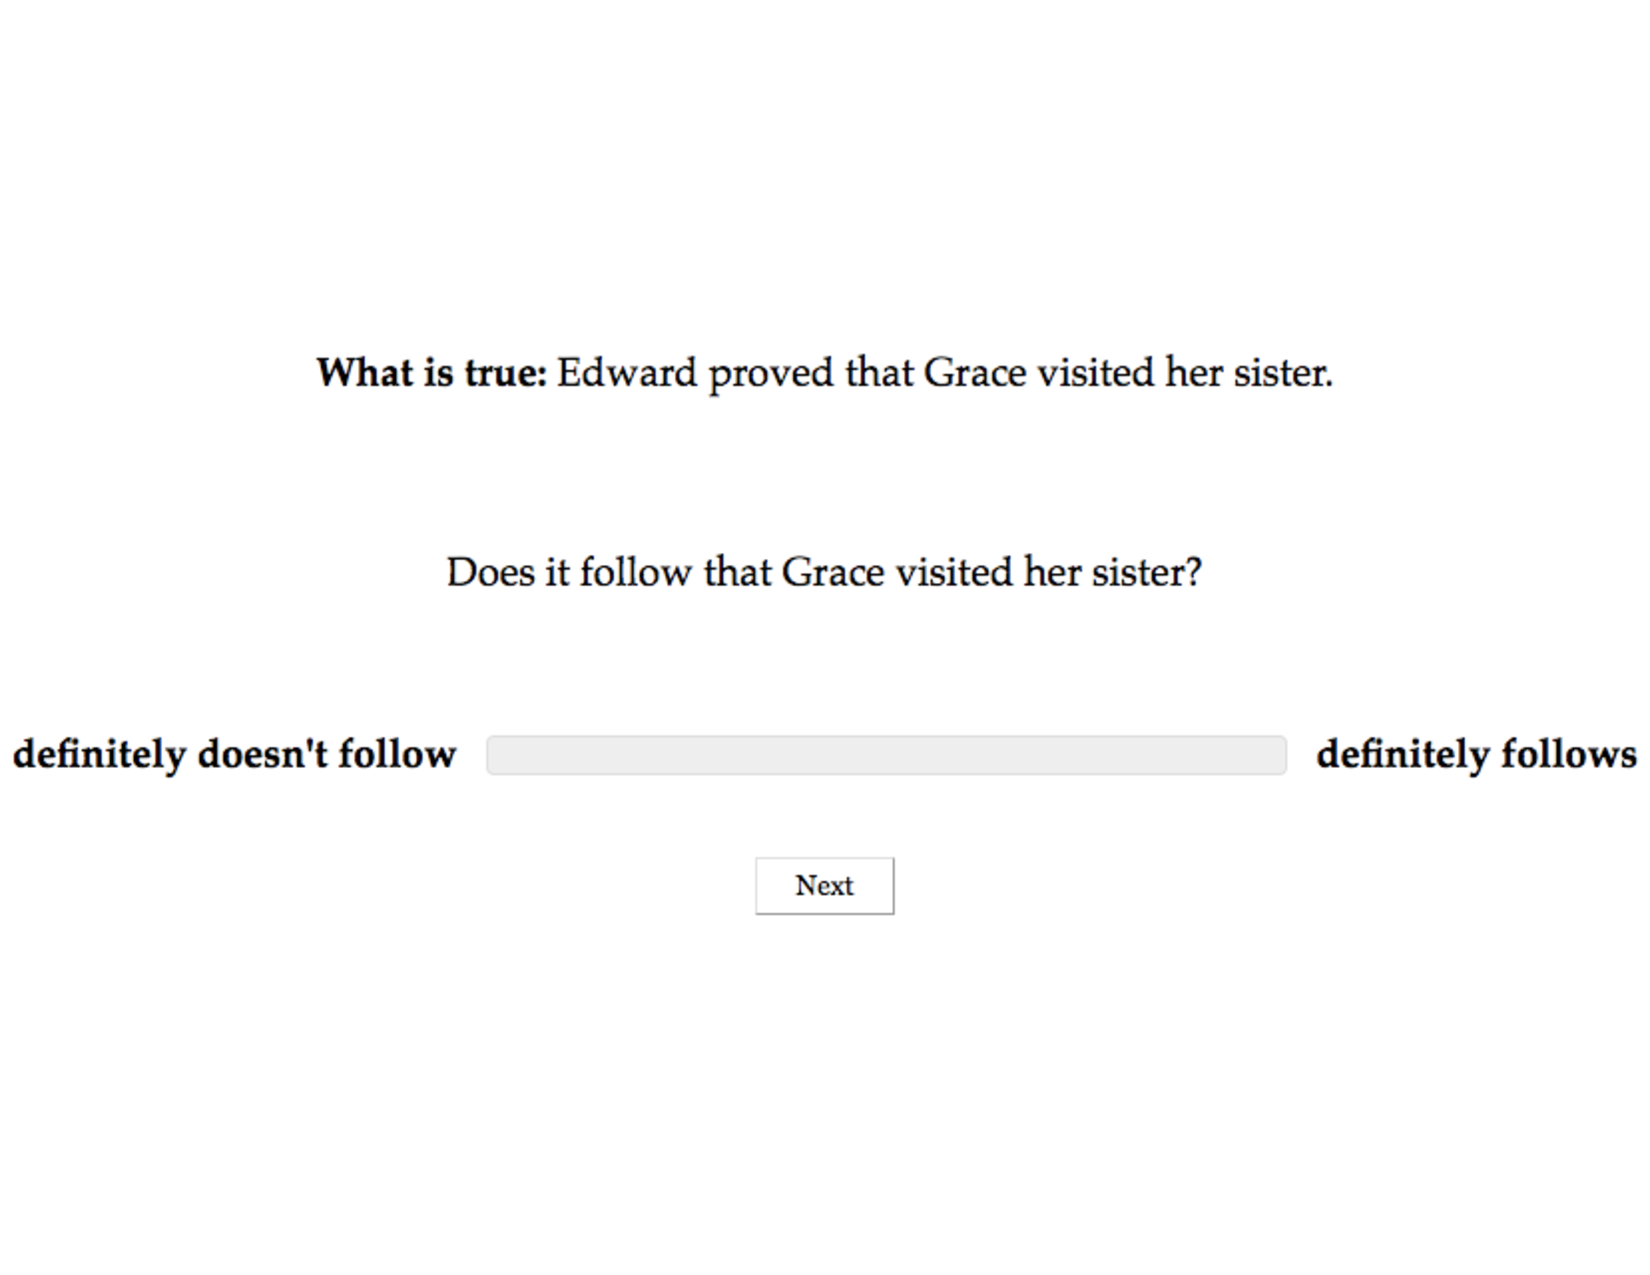
\includegraphics[width=13cm]{figures/inference-trial}}
\end{center}
\caption{A sample trial in Experiment 2a}\label{f-trial-exp3}
\end{figure}

To familiarize participants with the task, they first responded to the two familiarization stimuli in (\ref{train2}), where the inference tested was the CC. Participants who rated (\ref{train2}a) in the lower half of the sliding scale or (\ref{train2}b) in the upper half of the sliding scale were given an explanation for why their answer was wrong. Participants could only advance to the 28 stimuli if they gave a plausible rating to the two familiarization stimuli, that is, a rating in the upper half of the scale for (\ref{train2}a) and in the lower half for (\ref{train2}b).

\begin{exe}
\ex\label{train2}
\begin{xlist}
\ex {\bf What is true:} Drew is correct that Patty lives in Canada. 

\ex {\bf What is true}: Drew believes that Patty lives in Canada.
\end{xlist}
\end{exe}

%After responding to the 28 stimuli, participants filled out a short, optional survey about their age, their gender, their native language(s) and, if English is their native language, whether they are a speaker of American English (as opposed to, e.g., Australian or Indian English). To encourage them to respond truthfully, participants were told that they would be paid no matter what answers they gave in the survey.

\paragraph{Data exclusion} The data from 41 participants were excluded according to the criteria given in Supplement \ref{a-excl}. The data from 259 participants (ages 19-69; median: 36; 132 female, 128 male) were analyzed.

%. Closer inspection revealed that these participants' responses to the control stimuli were systematically higher or lower, respectively, suggesting that these participants did not attend to the task or interpreted the task differently. The data from these 27 participants were also excluded. In this experiment, we did not identify any participants who always selected roughly the same point on the response scale.  %; the group means were .96 for the control stimuli in (\ref{control-good2}) and .03 for the control stimuli in (\ref{control-bad2}).

\subsubsection{Results}


Figure \ref{f-veridicality-predicate} shows the mean inference ratings for the target stimuli by predicate, in increasing order from left to right, as well as for the non-entailing and entailing controls. In line with impressionistic judgments reported in the literature, the mean inference ratings for most factive predicates as well as the veridical non-factive predicate {\em be right} were quite high, suggesting strong inferences to the truth of the CC. The mean inference ratings of the purportedly factive predicate {\em reveal} and of the purportedly veridical non-factive predicate {\em demonstrate} were lower, suggesting comparatively weaker inferences to the truth of the CC. 

\begin{figure}[h!]
\centering

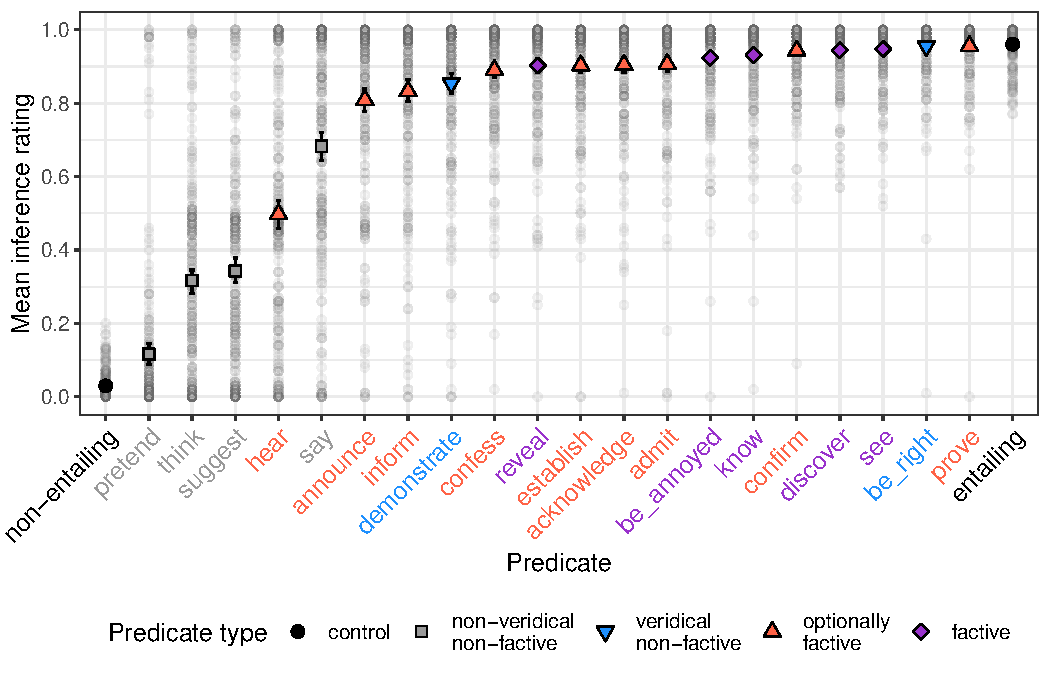
\includegraphics[width=.7\paperwidth]{../../results/4-veridicality3/graphs/means-inference-by-predicate-variability}

\caption{Mean inference rating by predicate in Exp.~2a, including the non-entailing and entailing controls. Error bars indicate bootstrapped 95\% confidence intervals. Light gray dots indicate individual participants' ratings.} 
\label{f-veridicality-predicate}
\end{figure}

To assess which predicates have entailed CCs, we fitted a Bayesian mixed effects Beta regression model  with weakly informative priors using the \verb|brms|  package in R that predicted the inference ratings from a fixed effect of predicate (with treatment coding and `entailing control' as  reference level) and included the maximal random effects structure justified by the design, random by-participant and by-item intercepts. According to this model, the estimated mean for each predicate except {\em prove} and {\em be right} was lower than that of the entailing controls, i.e., the 95\% credible intervals for the estimated adjustment to the intercept mean did not contain 0 for any predicate other than {\em prove} and {\em be right}. See Supplement \ref{a-mo} for the full model output.\footnote{A Bayesian mixed effects linear regression with the same fixed and random effects structure yielded similar results, except that in addition to {\em prove} and {\em be right}, there was no evidence for a difference between the entailing controls and \emph{know, confirm, discover} and {\em see}. See the Github repository mentioned in footnote \ref{f-github} for the model output.} Thus, the gradient inference ratings for the CCs of {\em be right} and {\em prove} are compatible with the assumption that their CCs are entailed. The inference ratings for the remaining predicates, including the factive predicates {\em see, discover, know, be annoyed} and {\em reveal} and the veridical non-factive predicate {\em demonstrate}, were significantly lower, suggesting that these CCs are not entailed, contrary to assumption. 



\subsubsection{Discussion}

The results of Exp.~2a have two unexpected implications. The first one concerns the predicates for which Exp.~2a found that their CCs are entailed, namely {\em be right} and {\em prove}. Given definition (\ref{def}b), according to which a predicate is factive if and only if its CC is presupposed and entailed, this means that these two predicates are factive if their CCs are presupposed. As discussed above, Exps.~1 found that the CCs of all 20 predicates investigated were at least mildly projective, compared to main clause content. We are therefore led to the conclusion that, according to the definition in (\ref{def}b), these two predicates are factive. This is a very unsatisfying conclusion because the CCs of these two predicates were among the least projective. 

The second unexpected implication concerns some of the predicates for which Exp.~2a found that their CCs are not entailed, namely {\em see, discover, know, be annoyed, reveal} and {\em demonstrate}. Under the definition of factive predicates in (\ref{def}b), this result means that, contrary to what is typically assumed, the predicates {\em see, discover, know, be annoyed} and {\em reveal} are not factive, nor is the predicate {\em demonstrate} veridical.

Our way of identifying entailed CCs, namely by comparing the CCs of the 20 predicates to entailed content, was motivated by the standard definition of entailment. One can, of course, ask whether there might be better ways of identifying entailed CCs. For instance, one might consider those CCs entailed whose mean inference rating was at least as high as that of {\em demonstrate} (.85): this would mean that the CCs of all of the predicates typically taken to be factive or veridical non-factive are entailed, as well as the CCs of some optionally factive predicates. There is, however, no principled reason why the rating for {\em demonstrate} should be the threshold for entailment. One could also pick an arbitrary mean inference rating, say .9, and categorize CCs with mean ratings of at least .9 as entailed, and CCs with mean ratings below .9 as not entailed. Of course, this way of identifying entailed CCs is also not principled. After all, one could just as well pick a threshold of .95 or .85, with the result that the CCs of different predicates would be considered entailed: for instance, the CC of {\em reveal} (.9) would count as entailed with a threshold of .85 but not with a threshold of .95. Furthermore, neither of these alternative ways of identifying entailed CCs are compatible with the standard definition of entailment because, under both, one would need to allow for CCs to count as entailed even though they received significantly lower ratings than entailed content.

%          verb       Mean       YMin       YMax
%1  acknowledge 0.90471042 0.88624807 0.92131660
%2        admit 0.90694981 0.88829633 0.92567761
%3     announce 0.80899614 0.77883687 0.83727606
%4   be_annoyed 0.92389961 0.90810618 0.93962162
%5     be_right 0.95509653 0.94319788 0.96548359
%6      confess 0.89019305 0.87007239 0.90965830
%7      confirm 0.94332046 0.93138031 0.95390347
%8  demonstrate 0.85378378 0.82782625 0.87772683
%9     discover 0.94447876 0.93331853 0.95467471
%10 entailing C 0.96077220 0.95600193 0.96480743
%11   establish 0.90289575 0.88297104 0.91989286
%12        hear 0.49776062 0.45794208 0.53757529
%13      inform 0.83262548 0.80188803 0.86197201
%14        know 0.93127413 0.91589768 0.94494402
%15  non-ent. C 0.02969112 0.02574131 0.03395849
%16     pretend 0.11617761 0.08848263 0.14606274
%17       prove 0.95583012 0.94443919 0.96583205
%18      reveal 0.90262548 0.88347104 0.92123745
%19         say 0.68277992 0.64300193 0.72162548
%20         see 0.94764479 0.93698745 0.95795753
%21     suggest 0.34254826 0.30826158 0.37788127
%22       think 0.31633205 0.28609846 0.34965347

It is also possible, however, that the surprising result of Exp.~2a---that {\em see, discover know, be annoyed} and {\em reveal} are not factive under definition (\ref{def}b)---is an artifact of the response task. For instance, the gradient response scale on which participants responded in Exp.~2a may have contributed to lower inference ratings for the CCs of these predicates, resulting in their classification as not entailed and, therefore, not factive under definition (\ref{def}b). To assess this possibility, we conducted Exp.~2b, which was identical to Exp.~2a but employed a two-alternative forced choice task.

\subsection{Exp.~2b: Categorical ratings using the inference diagnostic for entailment}

\subsubsection{Methods}

\paragraph{Participants} 600 participants with U.S.\ IP addresses and at least 99\% of previous HITs approved were recruited on Amazon's Mechanical Turk platform. They were paid \$1.

\paragraph{Materials and procedure} The materials and procedure were identical to those of Exp.~2a, with the exception of the task: participants responded `yes' or `no' to the question of whether the CC follows from the true statement, as shown in Figure \ref{fig-trial-exp2b}.

\begin{figure}[h!]
\begin{center}
\fbox{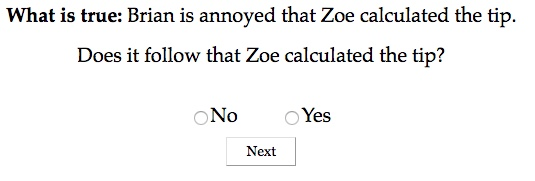
\includegraphics[width=10cm]{figures/Exp2b-trial}}
\end{center}
\caption{A sample trial in Experiment 2b}\label{fig-trial-exp2b}
\end{figure}


\paragraph{Data exclusion} The data from 225 participants were excluded according to the criteria given in Supplement \ref{a-excl}. The data from 375 participants (ages 18-73; median: 38; 187 female, 187 male, 1 undeclared) were analyzed.
    

\subsubsection{Results and discussion}

Figure \ref{fig:2bresults} shows the proportion of `yes' ratings by predicate, in increasing order from left to right, as well as on non-entailing and entailing controls. The results were strikingly similar to those of Exp.~2a: the proportions of `yes' responses were quite high for most factive predicates as well as for the veridical non-factive predicate {\em be right}, but lower for the purportedly factive predicate {\em reveal} and the purportedly veridical non-factive predicate {\em demonstrate}. The ordering of the predicates is almost entirely identical to the gradient measure of Exp.~2a, as evidenced by the very high Spearman rank correlation of .989 between Exps.~2a and 2b (see Supplement \ref{a-comparison} for a visualization). 
 
\begin{figure}[h!]
\centering
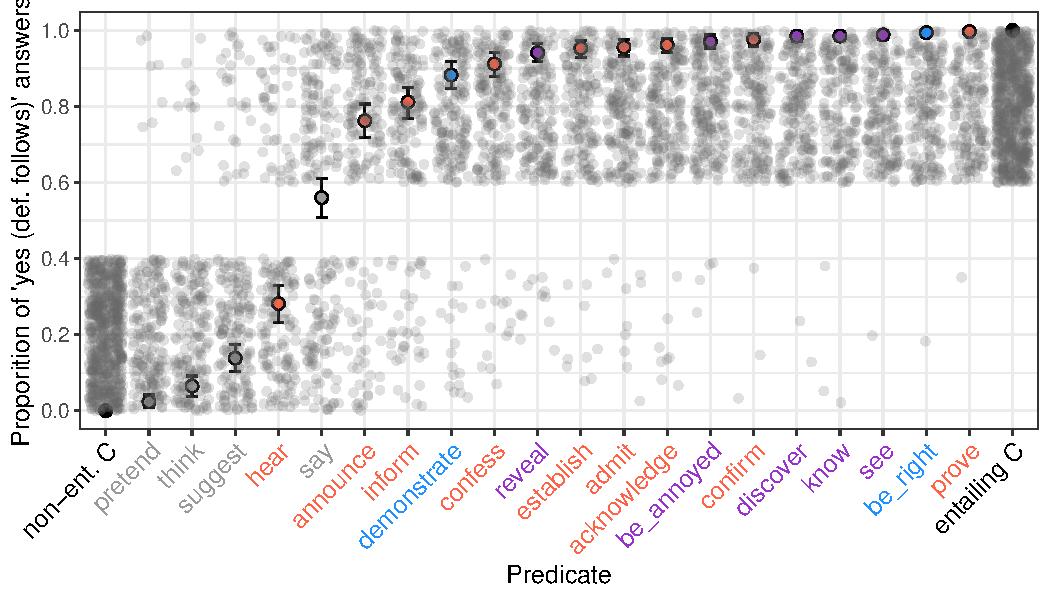
\includegraphics[width=.7\paperwidth]{../../results/7-veridicality3-binary/graphs/proportion-by-predicate-variability-individual}

\caption{Proportion of `yes' responses by predicate in Exp.~2b. Error bars indicate 95\% bootstrapped confidence intervals. Vertically jittered light gray dots indicate individual participants' responses of `yes' (coded as 1) and `no' (coded as 0).}
\label{fig:2bresults}
\end{figure}

To assess which predicates have entailed CCs, we fitted a Bayesian mixed effects logistic regression model with weakly informative priors using the \verb|brms|  package in R that predicted the log odds of a `yes' over a `no' response from a fixed effect of predicate (with treatment coding and `entailing control' as  reference level) and included the maximal random effects structure justified by the design, random by-participant and by-item intercepts. The estimated log odds of a `yes' response was lower for each predicate than for the entailing controls, i.e., the 95\% credible intervals for the estimated coefficients did not contain 0 for any predicate, except for {\em prove, be right, know, see, discover} and {\em confirm}. Thus, the categorical inference ratings for the CCs of {\em prove, be right, know, see, discover} and {\em confirm} are compatible with the assumption that the CCs of these predicates are entailed. The categorical inference ratings for the remaining predicates, including the factive predicates {\em be annoyed} and {\em reveal} and the veridical non-factive predicate {\em demonstrate}, were significantly lower, suggesting that these CCs are not entailed, contrary to assumption. 

Changing the response task from a gradient one (Exp.~2a) to a categorical one (Exp.~2b) resulted in slightly different conclusions: whereas Exp.~2a only supports the assumption that the CCs of {\em be right} and {\em prove} are entailed, Exp.~2b additionally supports the assumption that the CCs of {\em know, see, discover} and {\em confirm} are entailed. However, the implications of Exp.~2b are just as unexpected as those of Exp.~2a. First, because the CCs of {\em confirm, discover, see, know, be right} and {\em prove} are entailed and projective, this set of predicates is identified, by the definition of factive predicates in (\ref{def}b), as factive. This is an unsatisfying conclusion because this set of predicates is very heterogeneous with respect to projection:  the CC of {\em be right} was among the least projective of the 20 predicates investigated while that of {\em know} was among the most projective. Thus, this set of predicates can hardly be considered a natural class. Second, the predicates {\em be annoyed} and {\em reveal} are  not factive under the definition of factive predicates in (\ref{def}b) and the predicate {\em demonstrate} is  not veridical. 

The results of both Exps.~2a and 2b have unexpected implications for the identification of factive predicates. One might ask whether these results and their implications are an artifact of the inference diagnostic for entailment. To assess this possibility, we conducted Exps.~3a and 3b, which were identical to Exps.~2a and 2b, respectively, but employed the contradictoriness diagnostic for entailment.

\subsection{Exp.~3a: Gradient ratings using the contradictoriness diagnostic for entailment}\label{s32}

Exp.~3a investigated which of the CCs of the 20 clause-embedding predicates are entailed, based on the contradictoriness diagnostic for entailment in (\ref{diag}b). Participants rated the contradictoriness of utterances of English sentences of the form {\em $\phi$ but not $\psi$}, where $\phi$ is an indicative matrix sentence with a clause-embedding predicate and $\psi$ is its clausal complement, as in (\ref{announce3}):

\begin{exe}
\ex\label{announce3} Mary announced that she is pregnant, but she's not.
\end{exe}
Gradient contradictoriness ratings were collected.

\subsubsection{Methods}

\paragraph{Participants} 300 participants with U.S.\ IP addresses and at least 99\% of previous HITs approved were recruited on Amazon's Mechanical Turk platform (ages: 18-72, median: 35; 137 female, 162 male, 1 other). They were paid \$0.75.

\paragraph{Materials} On target trials, the 400 predicate/clause combinations were combined with a proper name subject and a {\em but-}clause that denied the truth of the CC. As shown in ({\ref{stims}), stimuli were presented to participants as utterances by named speakers. The proper names that realized the speakers, the subjects of the 20 predicates and the subjects of the complement clauses were all unique. The gender of the proper name subject of the predicate was distinct from the gender of the proper name in the complement clause, to ensure that the pronoun in the elliptical {\em but-}clause unambiguously referred to the individual in the complement clause.

\begin{exe}
\ex\label{stims}
\begin{xlist}
\ex {\bf Christopher:} {\em ``Melissa knows that Danny ate the last cupcake, but he didn't.''}
\ex {\bf Susan:} {\em ``Jerry pretended that Emma studied on Saturday morning, but she didn't.''}
\end{xlist}
\end{exe}

The experiment  included eight control stimuli that were used to assess whether participants were attending to the task, as well as to identify contradictoriness ratings for entailed content. There were four control stimuli, like (\ref{control-bad}), for which we expected contradictoriness ratings to be at ceiling because the first clause of each of these sentences entails the negation of the second clause. In (\ref{control-bad}), for instance, the content of {\em Madison laughed loudly} entails that Madison laughed, that is, the negation of {\em she didn't laugh}. As discussed above, we relied on the contradictoriness ratings for these control stimuli to identify entailments. By contrast, we expected the contradictoriness ratings for the four non-contradictory control stimuli, like (\ref{control-good}), to be at floor, because the content of the second clause does not contradict the content of the first clause. For instance, in (\ref{control-good}), the content that Vanessa is good at math does not entail the negation of the content that the speaker is not good at math. For the full set of control stimuli see Supplement \ref{a-control}.

\begin{exe}

\ex\label{control-bad} Madison laughed loudly and she didn't laugh.
\ex\label{control-good}  Vanessa is really good at math, but I'm not.
\end{exe}

Each participant saw a random set of 28 stimuli: each set contained one target stimulus for each of the 20 predicates (each with a unique complement clause) and the same 8 control stimuli. Trial order was randomized.


\paragraph{Procedure.} Participants were told that they would read utterances produced by a speaker and were asked to assess whether the utterance is contradictory. On each trial, participants read the speaker's utterance and then gave their response on a slider marked `definitely no' at one end (coded as 0) and `definitely yes' at the other (coded as 1), as shown in Figure \ref{f-trial-exp2}. Participants first responded to two familiarization stimuli.

\begin{figure}[h!]
\begin{center}
\fbox{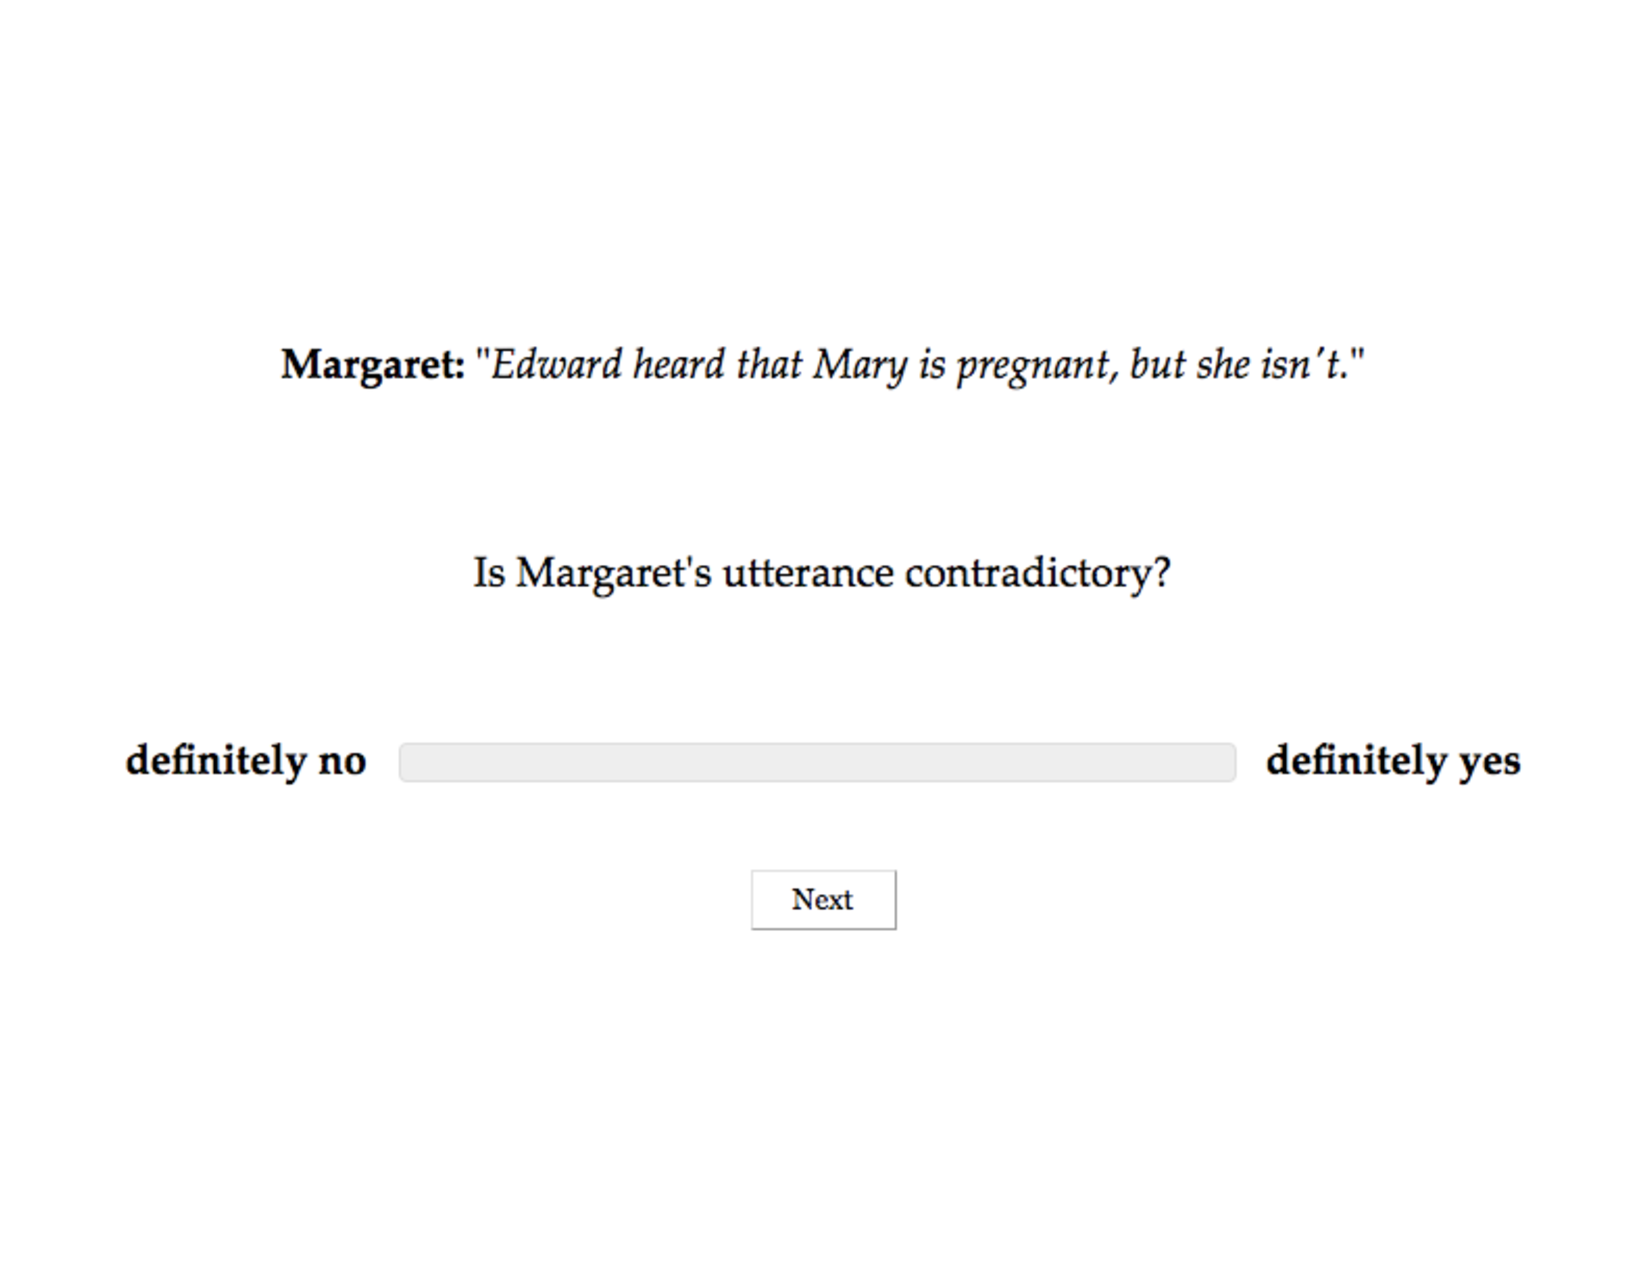
\includegraphics[width=13cm]{figures/contradictory-trial}}
\end{center}
\caption{A sample trial in Experiment 3a}\label{f-trial-exp2}
\end{figure}

%To familiarize participants with the task, they first responded to the two familiarization stimuli in (\ref{train}): participants who rated (\ref{train}a) in the lower half of the scale or (\ref{train}b) in the upper half of the scale were given an explanation for why their answer was wrong. Participants could only advance to the 28 stimuli if they gave a plausible rating to the two training stimuli, that is, a rating in the upper half of the scale for (\ref{train}b) and a rating in the lower half for (\ref{train}b).
%
%\begin{exe}
%\ex\label{train}
%\begin{xlist}
%\ex Drew is aware that Patty lives in Canada, but she doesn't.
%
%\ex Drew thinks that Patty lives in Canada, but she doesn't.
%\end{xlist}
%\end{exe}

%After responding to the 28 stimuli, participants filled out a short, optional survey about their age, their gender, their native language(s) and, if English is their native language, whether they are a speaker of American English (as opposed to, e.g., Australian or Indian English). To encourage them to respond truthfully, participants were told that they would be paid no matter what answers they gave in the survey.

\paragraph{Data exclusion} The data from 37 participants were excluded according to the criteria given in Supplement \ref{a-excl}. The data from 263 participants (ages 18-72; median: 36; 126 female, 136 male, 1 other) were analyzed.

\subsubsection{Results and discussion}


Figure \ref{f-veridicality-predicate2} shows the mean contradictoriness ratings for the target and control stimuli. In line with impressionistic judgments reported in the literature, the mean inference ratings for the factive and veridical non-factive predicates were among the highest, and those of the non-factive non-veridical predicates were among the lowest. However, except possibly for {\em be right}, none of the mean contradictoriness ratings were close to those of the contradictory controls.

%   verb              Mean
%   <chr>            <dbl>
% 1 acknowledge     0.672 
% 2 admit           0.711 
% 3 announce        0.448 
% 4 be_annoyed      0.640 
% 5 be_right        0.941 
% 6 confess         0.669 
% 7 confirm         0.767 
% 8 contradictory C 0.960 
% 9 demonstrate     0.720 
%10 discover        0.789 
%11 establish       0.721 
%12 hear            0.238 
%13 inform          0.472 
%14 know            0.838 
%15 non-contrd. C   0.0587
%16 pretend         0.217 
%17 prove           0.858 
%18 reveal          0.634 
%19 say             0.363 
%20 see             0.819 
%21 suggest         0.257 
%22 think           0.171 

\begin{figure}[h!]
\centering

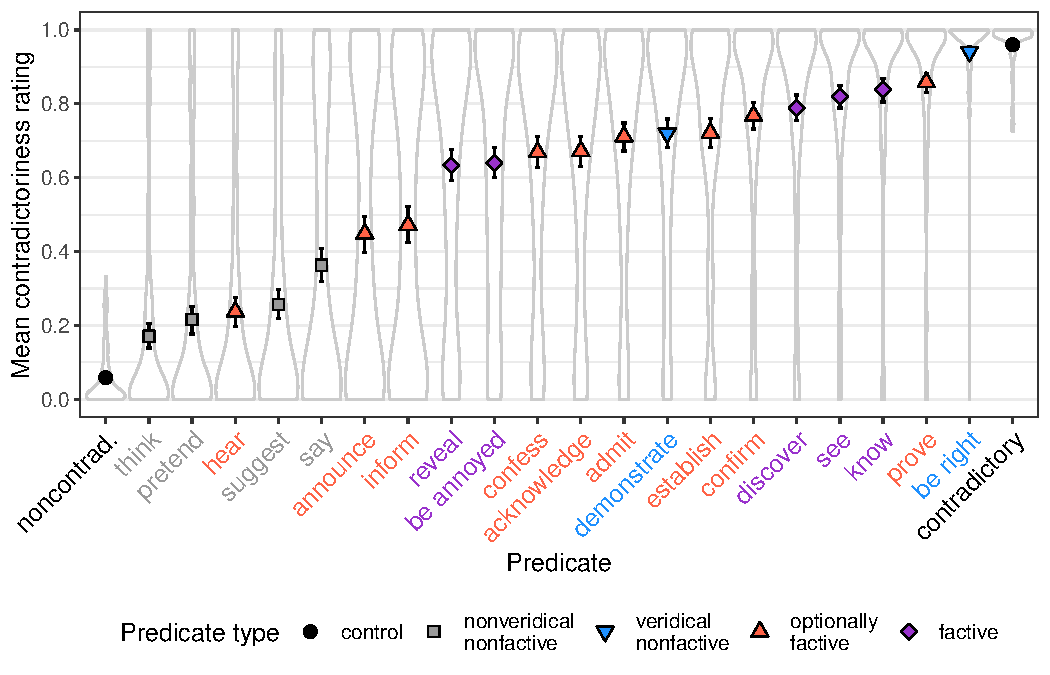
\includegraphics[width=.7\paperwidth]{../../results/2-veridicality2/graphs/means-contradictoriness-by-predicate-variability}

\caption{Mean contradictoriness rating by predicate in Exp.~3a, including the non-contradictory and contradictory controls. Error bars indicate bootstrapped 95\% confidence intervals. Light gray dots indicate individual participants' ratings.}
\label{f-veridicality-predicate2}
\end{figure}

To assess which predicates have entailed CCs, we fitted a Bayesian mixed effects Beta regression model  with weakly informative priors using the \verb|brms|  package in R that predicted the contradictoriness ratings from a fixed effect of predicate (with treatment coding and contradictory control as  reference level) and included the maximal random effects structure justified by the design, random by-participant and by-item intercepts. According to this model, the estimated mean for all predicates was lower than that of the contradictory controls, i.e., the 95\% credible intervals for the estimated adjustment to the intercept mean did not contain 0 for any predicate. See Supplement \ref{a-mo} for the full model output.\footnote{A Bayesian mixed effects linear regression with the same fixed and random effects structure yielded qualitatively identical results, except that the contrast between \emph{be right} and the contradictory controls was not significant. See the Github repository mentioned in footnote \ref{f-github} for the model output.} Thus, the gradient contradictoriness ratings for none of the predicates are compatible with the assumption that the CCs are entailed and, consequently, none of the 20 predicates are factive under the definition in (\ref{def}b). 

Given the difference in results for Exps.~2a and 2b, one may again ask whether the lack of entailed CCs identified by Exp.~3a is an artifact of the gradient response task, and whether categorical responses might result in more CCs being classified as entailed. To assess this possibility, we conducted Exp.~3b, which was identical to Exp.~3a but employed a two-alternative forced choice task.

%Contextual factors may influence contradictoriness ratings: for instance, how contradictory an utterance of (\ref{announce3}) is assessed to be may depend on how old or how trustworthy Mary is (see, e.g., \citealt{schlenker10,demarneffe-etal2012}). To allow participants' ratings to reflect degrees of contradictoriness, we collected gradient contradictoriness ratings. We assume that when the content of $\phi$ entails the content of $\psi$, the contradictoriness of an utterance of the form {\em $\phi$ but not $\psi$} is not mitigated by contextual factors, and participants' contradictoriness ratings are at ceiling, that is, indistinguishable from contradictory control stimuli.


\subsection{Exp.~3b: Categorical ratings using the contradictoriness diagnostic for entailment}\label{s32}

\subsubsection{Methods}

\paragraph{Participants} 600 participants with U.S.\ IP addresses and at least 99\% of previous HITs approved were recruited on Amazon's Mechanical Turk platform. They were paid \$1.

\paragraph{Materials and procedure} The materials and procedure were identical to those of Exp.~3a, with the exception of the task: participants responded `yes' or `no' to the question of whether the speaker's utterance is contradictory, as shown in Figure \ref{fig-trial-exp3b}.

\begin{figure}[h!]
\begin{center}
\fbox{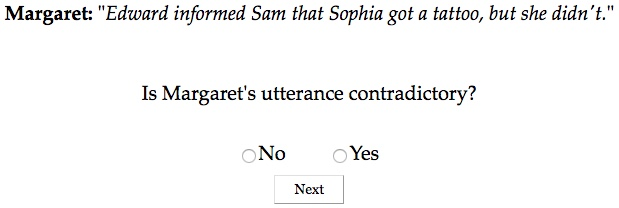
\includegraphics[width=10cm]{figures/Exp3b-trial}}
\end{center}
\caption{A sample trial in Experiment 3b}\label{fig-trial-exp3b}
\end{figure}


\paragraph{Data exclusion} The data from 247 participants were excluded according to the criteria given in Supplement \ref{a-excl}. The data from 353 participants (ages 18-73; median: 37; 180 female, 173 male) were analyzed.
    


\subsubsection{Results and discussion}

Figure \ref{fig:3bresults} shows the proportion of `yes' responses on target and control trials. The results of Exp.~3b were very similar to those of Exp.~3a: except possibly for {\em be right}, the contradictoriness ratings for the CCs of none of the predicates were close to the contradictory controls. The Spearman rank correlation between Exps.~3a and 3b was very high, at .985 (see Supplement \ref{a-comparison} for a visualization).

\begin{figure}[h!]
\centering
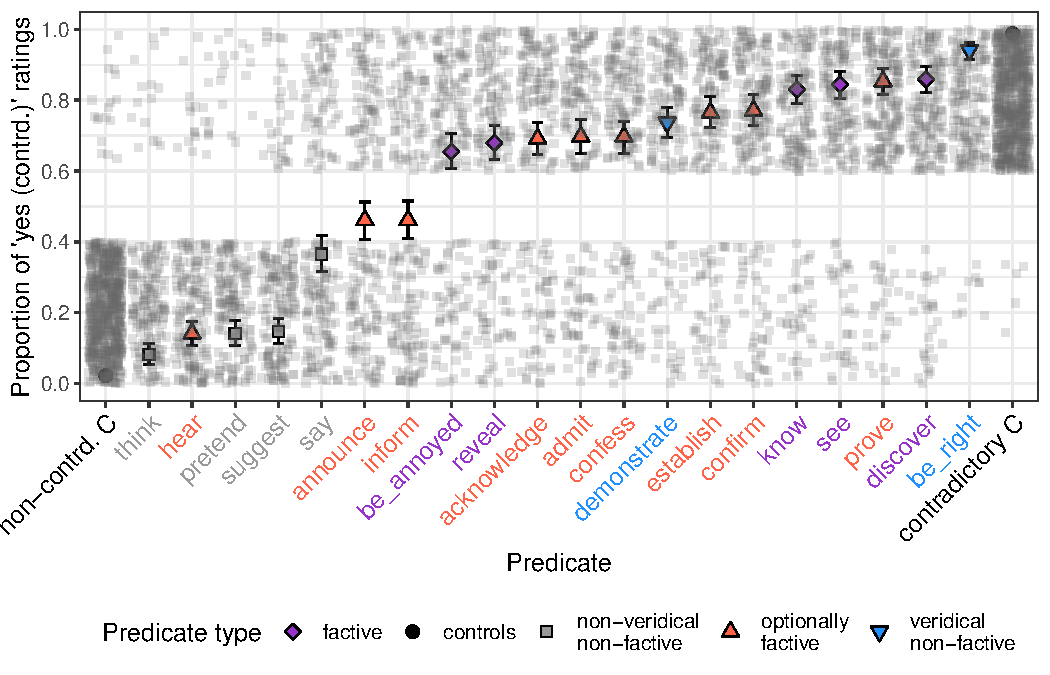
\includegraphics[width=.7\paperwidth]{../../results/6-veridicality2-binary/graphs/proportion-by-predicate-variability-individual}
\caption{Proportion of `yes' ratings by predicate in Exp.~3b. Error bars indicate 95\% bootstrapped confidence intervals. Vertically jittered light gray dots indicate individual participants' ratings of `yes' (coded as 1) and `no' (coded as 0). }
\label{fig:3bresults}
\end{figure}

To assess which predicates have entailed CCs, we fitted a Bayesian mixed effects logistic regression model with weakly informative priors using the \verb|brms|  package in R that predicted the log odds of a `yes' over a `no' response from a fixed effect of predicate (with treatment coding and `contradictory control' as  reference level) and included the maximal random effects structure justified by the design, random by-participant and by-item intercepts. The estimated log odds of a `yes' response was lower for each predicate than for the contradictory controls, i.e., the 95\% credible intervals for the estimated coefficients did not contain 0 for any predicate. Thus, as with Exp.~3a, the results of Exp.~3b suggest that the CCs of none of the 20 predicates are entailed. Consequently, as with Exp.~3a, none of the 20 predicates are factive under the definition of factive predicates in (\ref{def}b). 

\subsection{Do projection and entailment jointly identify a class of factive predicates?}\label{s33}

According to definition (\ref{def}b), a predicate is factive if and only if its CC is presupposed and entailed. In Exps.~2 and 3, we compared the inference ratings (Exps.~2) and the contradictoriness ratings (Exps.~3) for the CCs to the ratings for control stimuli with entailed content. We found that the CCs of {\em prove} and {\em be right} are entailed based on the gradient and the categorical inference diagnostic (Exps.~2a and 2b), that the CCs of {\em see, discover} and {\em confirm} are entailed based on the categorical inference diagnostic (Exp.~2b) but not on the gradient one (Exp.~2a), and that the CCs of none of the 20 predicates are entailed based on the gradient and categorical contradictoriness diagnostics for entailment (Exps.~3).\footnote{The differences in the results of Exps.~2 and 3 highlight the importance for future research to investigate the validity of entailment diagnostics. While the ratings were overall lower with the  contradictoriness diagnostic than the inference diagnostic, the high Spearman rank correlations between the ratings from the two diagnostics---.954 for the two gradient measures and .934 for the two categorical measures---suggests that both are measuring a similar underlying concept. Moreover, the entailed controls received very high ratings across Exps.~2 and 3, suggesting that all four measures are able to diagnose entailed content with some reliability.   However, \citet[329]{demarneffe-etal2012} have suggested that veridicality ratings (comparable to our inference ratings) are influenced by pragmatic reasoning; see also \citealt{pavlick-kwiatkowski2019}.}} Given that the CCs of all 20 predicates are at least mildly projective, this means, under definition (\ref{def}b), that the predicates {\em prove} and {\em be right} are factive according to the results of Exp.~2a, that the predicates {\em prove, be right, know, see, discover} and {\em confirm} are factive according to the results of Exp.~2b, and that none of the 20 predicates are factive according to the results of Exps.~3.  

\jt{We conclude that definition (\ref{def}b) also does not identify a class of factive predicates.} First, given the results of the gradient inference diagnostic (Exp.~2a), the predicates {\em be right} and {\em prove} are factive, but it is unsatisfying to consider them factive predicates because they both have only weakly projective CCs. Second, given the results of the categorical inference diagnostic (Exp.~2b), the predicates {\em prove, be right, see, discover, confirm} and possibly {\em know} are factive, but this is a heterogeneous set of predicates and not a natural class: the CC of {\em be right} was among the least projective and that of {\em know} was among the most projective. Finally, given the results of the contradictoriness diagnostic, none of the 20 predicates is factive. In short, the set of predicates identified as factive is either heterogeneous with respect to projection, i.e., not a natural class, or empty. 

Converging evidence for this conclusion comes from the VerbVeridicality and MegaVeridicality datasets. Consider first the VerbVeridicality dataset: in addition to projection ratings for the CCs of the negated variants of the 859 indicative matrix sentences, it also contains entailment ratings for the 859 indicative matrix sentences; an example is given in (\ref{vv-stim-proj2}). 

\begin{exe}
\ex\label{vv-stim-proj2} The GAO has indicated that it is unwilling to compromise.  \hfill (\citealt[2234]{ross-pavlick2019})
\end{exe}
To diagnose entailment, three participants rated on a 5-point Likert scale whether the CC is true given the target sentence; one endpoint of the scale was labeled `definitely true' (coded as 2) and the other `definitely not true' (coded as -2). We follow \citet{ross-pavlick2019} in referring to these as `veridicality' ratings. 

Figure \ref{f-vv-projectivity} plots the mean veridicality ratings for the 78 clause-embedding predicates in the VerbVeridicality dataset, with labels for the 15 predicates from our experiments (recall that {\em see} and {\em saw} are plotted separately). On the standard definition of entailment, predicates with entailed CCs should have a mean veridicality rating of 2. None of the clause-embedding predicates have a mean veridicality rating of 2: thus, the CCs of none of these 78 clause-embedding predicates are entailed and, consequently, none of the 78 predicates are factive according to the definition in (\ref{def}b). Relaxing the linking function results in a heterogeneous set of factive predicates: For instance, there are 15 predicates whose CC received a mean veridicality rating at least as high as that of {\em know} (1.5). If one assumes that these CCs are entailed and that CCs with mean projection ratings of at least .3 are presupposed,\footnote{The VerbVeridicality dataset does not include projection ratings for main clause content to which the projection ratings for the CCs could be compared. The cutoff of a mean projection rating of .3 (on a scale from -2 to 2) is arbitrary but comparable to the mean certainty rating of .15 (on a scale from 0 to 1) for {\em pretend} in our Exp.~1a.} then the set of factive predicates is heterogeneous with respect to projection: it includes {\em notice}, with a mean projection rating of 1.1, {\em give} (1.1), {\em realize} (1.1), {\em explain} (.9) and {\em know} (.8), but also {\em acknowledge} (.5), {\em learn} (.4), {\em saw} (.4) and {\em admit} (.3). In short, on the VerbVeridicality set, too, \jt{definition (\ref{def}b) of factive predicates fails to identify a class of factive predicates.}

\begin{figure}[H]
\centering
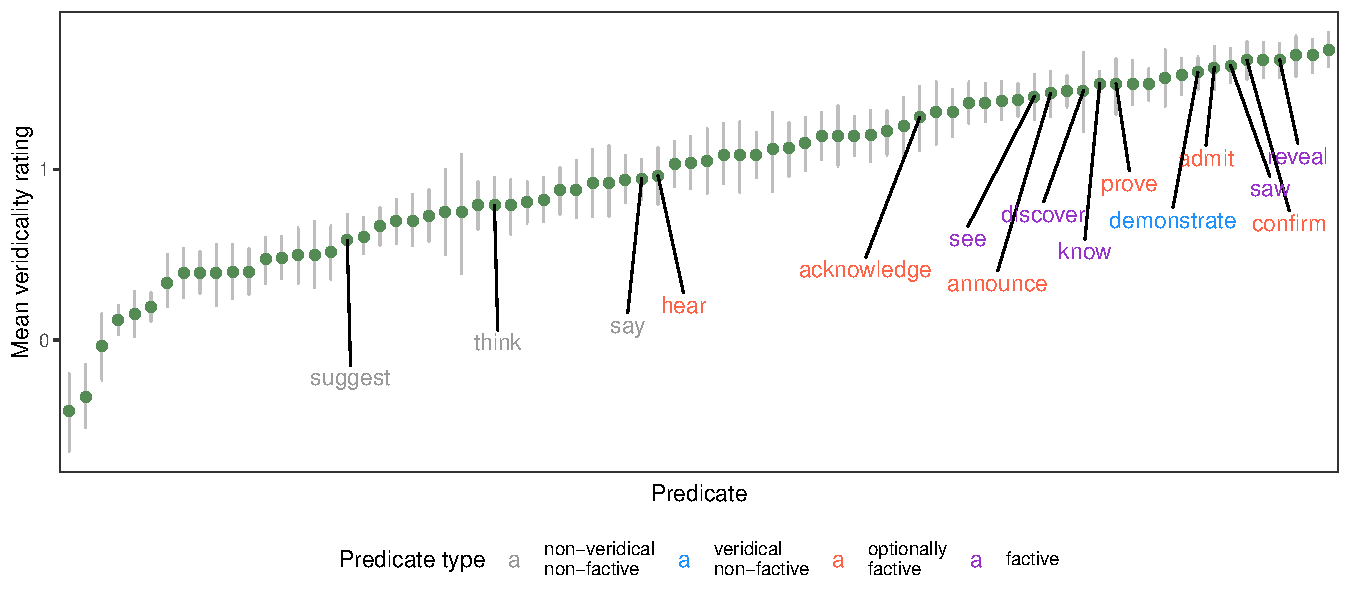
\includegraphics[width=.77\paperwidth]{../../VerbVeridicality-analysis/graphs/means-entailment-by-predicate}

\caption{Mean veridicality rating by predicate in green, with 95\% bootstrapped confidence intervals, for the 78 predicates in the VerbVeridicality dataset (\citealt{ross-pavlick2019}), with labels for the 15 predicates featured in our experiments.}
\label{f-vv-projectivity}
\end{figure}

The MegaVeridicality dataset includes veridicality ratings for the CCs of the same 517 English clause-embedding predicates for which projection ratings were collected. The veridicality ratings were collected for stimuli that combined these predicates with arguments with low lexical content, as shown in (\ref{wr-stim-ent}) for the predicate {\em know}. To diagnose veridicality, participants were asked to respond to the question {\em Did that thing happen?}; the response options were `yes' (which we again coded as 1), `maybe or maybe not' (0) and `no' (-1).

\begin{exe}
\ex\label{wr-stim-ent} Somebody knew that a particular thing happened.
\end{exe}

Each of the 517 predicates in the MegaVeridicality dataset received between 9 and 20 entailment ratings (mean: 10) from 159 participants. Figure \ref{f-white-rawlins-ent} plots the mean veridicality ratings, with labels for the 19 predicates from our experiments. On the standard definition of entailment, one would expect predicates with entailed CCs to have a mean veridicality rating of 1. There are 97 clause-embedding predicates that only received `yes'/1 ratings, including 3 of the factive predicates we investigated, namely {\em reveal, know} and {\em be annoyed}; this result is compatible with the assumption that the CCs of these 97 predicates are entailed.\footnote{\label{mv}It is not clear that the CCs of these 97 predicates are entailed: this set includes {\em inform} (see the discussion in section \ref{s1}) as well as the communication predicates {\em bitch} and {\em howl}, whose CCs are not entailed. 
For instance, it does not follow indefeasibly from the naturally occurring example with {\em bitch} in (i) that the Democratic party hates all the Jews.
\begin{exe}
\exi{(i)} Rambling to reporters in the Oval Office, Trump bitched that the Democratic party clearly hates all the Jews because of all the support reps Rashida Tlaib and Ilhan Omar received after he strong armed the Israelis into barring them from visiting the country as members of Congress. (\url{https://www.wonkette.com/08-21-2019})
\end{exe}
}
%\citet{white-rawlins-nels2018} assumed that the CCs of 376 of the 517 predicates are entailed because they assumed that the CC of a predicate is entailed if and only if the majority of the responses for a predicate was `yes'. We do not adopt this linking function because it is incompatible with the standard definition of entailment: for instance, given this linking function, the CC of {\em tweet} is entailed because 11 of the 20 participants responded `yes', despite the remaining 9 participants responding `maybe or maybe not'.} 
If we assume, again, that CCs with mean projection ratings of at least .3 are presupposed, then 92 of the 97 predicates are factive. This set is heterogeneous with respect to projection, including predicates like {\em bother}, with a mean projection rating of .97, {\em inform} (.7), {\em know} (.63), {\em grumble} (.5), {\em notify} (.4), {\em gloat} (.4) {\em convey} (.4) and {\em confirm} (.3). \jt{Thus, on the MegaVeridicality set, too, definition (\ref{def}b) fails to identify a class of factive predicates. }
 
 This conclusion dovetails with that of \citet{white-rawlins-nels2018}, who assumed definition (\ref{def}b). They pointed out (p.228) that if one were to assume a majority response as threshold for whether the CC is presupposed and entailed, there are 199 factive and 292 non-factive predicates in the MegaVeridicality dataset, but also that ``there are not necessarily clear dividing lines between these classes present in the data, suggesting that speaker's inferences about [projection and entailment; the anonymous authors] are generally quite gradient and likely influenced by the fine-grained semantics
of particular verbs''.

\begin{figure}[H]
\centering
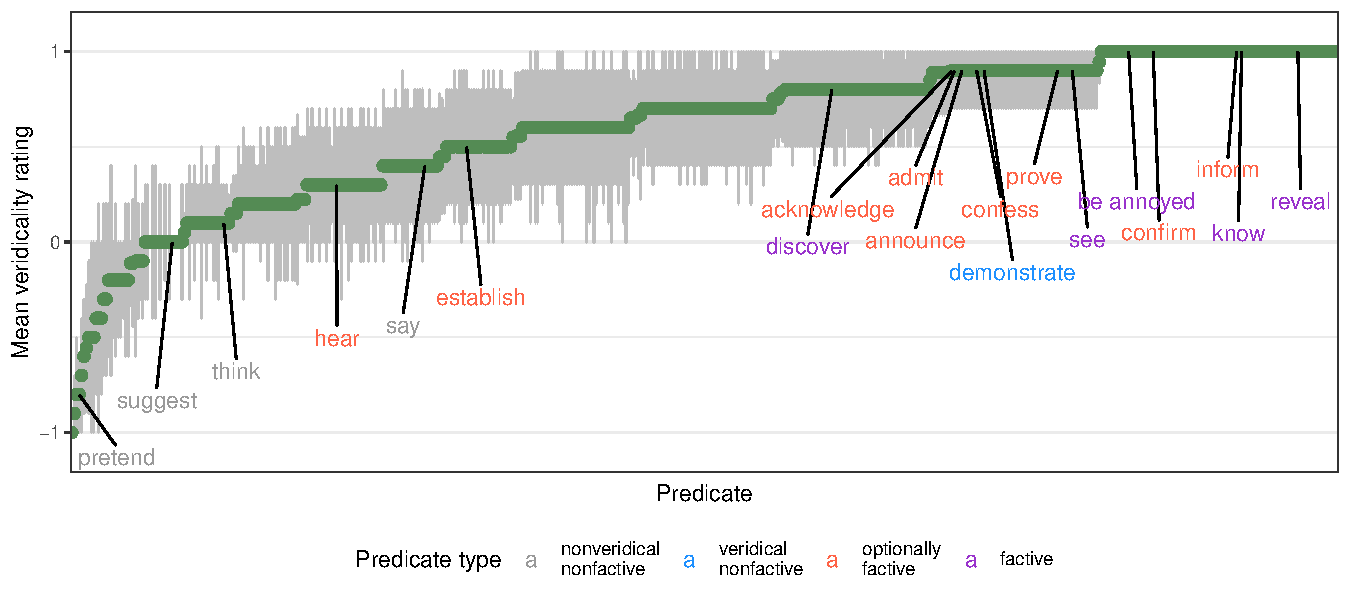
\includegraphics[width=.75\paperwidth]{../../MegaVeridicality-analysis/graphs/means-entailment-by-predicate}

\caption{Mean veridicality rating by predicate in green, with 95\% bootstrapped confidence intervals, for the 517 predicates in the MegaVeridicality dataset (\citealt{white-rawlins-nels2018,white-etal2018b}), with labels for the 19 predicates featured in our experiments.}
\label{f-white-rawlins-ent}
\end{figure}

In sum, contrary to what is expected under the definition of factive predicates in (\ref{def}b), the results of our Exps.~1, 2 and 3, as well as those of the VerbVeridicality and MegaVeridicality datasets, \jt{suggest that projection and entailment of the CC do not jointly identify a class of factive predicates.} Depending on how entailment is diagnosed and which linking function is assumed, the set of predicates identified as factive is either heterogeneous with respect to projection or empty. 

\section{General discussion}\label{s4}

Factivity has played a central role in linguistic theorizing on topics such as projection, the interpretation of embedded questions, extraction and island effects, control and mood (for more topics and references see section \ref{s1}). Despite this central role, there is no agreement in the literature about how factive predicates are defined and which predicates are factive. In sections \ref{s2} and \ref{s3}, we reported the results of experiments designed to investigate whether two prevalent definitions identify a class of factive predicates. Our experiments in section \ref{s2} investigated the definition in (\ref{def}a), according to which a predicate is factive if and only if its CC is presupposed. The results of these experiments and the meta-analyses of three existing datasets suggest that projection does not identify a class of factive predicates. In section \ref{s3}, we investigated the definition in (\ref{def}b), according to which a predicate is factive if and only if its CC is both presupposed and entailed. We found that, depending on how entailment is diagnosed, there are either no factive predicates or that the set of predicates identified as factive is heterogeneous with respect to projection, i.e., not a natural class. 

In this section, we discuss what evidence for a class of factive predicates might look like (section \ref{s41}), what our results mean for projection analyses (section \ref{s42}), and what we take to be fruitful avenues for future research on projective content (section \ref{s43}).

\subsection{On the relation between gradient judgments and linguistic categories}\label{s41}

\begin{itemize}

\item Factivity has traditionally been taken to impose a binary categorization on predicates, most often a binary one. 

\begin{exe}
\exi{(\ref{def})} Two definitions of factive predicates \\ A clause-embedding predicate is factive if and only if the content of its clausal complement is 
\begin{xlist}
\ex presupposed. \hfill (e.g., \citealt{kiparsky-kiparsky70,karttunen71-implicative,karttunen71b})
\ex presupposed and entailed.  \hfill (e.g., \citealt{gazdar79a,schlenker10,abrusan2011}\\\hspace*{.2cm}\hfill \citealt{anand-hacquard2014,spector-egre2015})
\end{xlist}
\end{exe}

\item Presupposition and entailment have also been taken to be binary categories: a content is either presupposed / entailed, or not.

\item We diagnose presupposition using projection inferences (specifically: certainty ratings). Projection inferences: we collect gradient ratings, to allow for gradience to show up, but we also collected binary ratings, gradience still shows up. Speaker commitment may be gradient or binary (we remain agnostic).

\item We diagnose entailment using inference and contradictoriness ratings. Inference ratings are gradient (we assume). We assume that contradictoriness is binary, but we also collect both gradient and binary ratings here.

\item We have observed gradience in certainty, inference, and contradictoriness ratings. To evaluate the definitions in (\ref{def}), we need to relate these gradient ratings to the categories.

\item What goes into establishing this relation, under the assumption of factive predicate class:

\begin{enumerate}

\item[0] Predicate (factive or not)

\item[i] combined with subject and complement clause

\item[ii] used in an utterance (speaker, context)

\item[iii] response question, response option

\item[iv] human rating

\end{enumerate}

If no noise was introduced at any of these points, we should expect to see two very distinct classes. 

Certainty ratings: two classes, by presupposed

Inference/contradictoriness: two classes, by veridicality.

But if there's noise, we expect to see gradience. 

We expect gradience: i) noise, ii) no underlying category.

The more systematic the gradience, the less likely it is to be noise. 

Certainty ratings: different entailment-canceling operators, different tasks, different sentence naturalness

Entailment: different tasks, different sentence naturalness

\item We can't just say that because there are gradient ratings that there is no factivity category because i) the predicate is used in a particular sentence, ii) the sentence was uttered by a named speaker, iii) we used a particular task to collect ratings (certainty, inference, contradictoriness), and iv) we collected ratings from humans. Each of i)-iv) can introduce systematic noise, which, one could hypothesize, created gradience even though the predicate is either factive or not (categorical).

\item We have done a number of things to mitigate the systematic noise introduced: i) same sentence structure, same CCs, ii) same utterance type (polar questions) in the same context, iii) compared ratings across different tasks, and iv) from lots of humans.

One might reject the conclusion on methodological or conceptual grounds. On the former, one might argue that the tasks introduced noise into the response behavior that is independent of the properties of the predicates, or that participants had uncertainty about whether a particular predicate is factive. While both are a possibility,  it is unclear how such arguments could explain the very similar qualitative order of predicates across  Exps.~1a, 2a, and 3a vs.~1b, 2b, and 3b, respectively. This is not enough to argue against option 1.

- Things that speak against option 1: systematicity in gradient orderings of predicates regardless of sentence type, natural, diagnostic...,

\item This is what makes us think that it is unlikely that there is a binary factivity category that is covered up by systematic noise.

\item But it is still a possibility. It is still possible that categorical factivity is being distorted in some systematic way.  

\item Therefore, we cannot rule out that there is no class. But the systematicity we have found is strongly suggestive of underlying gradience.

Things one can do: mixture models.

One approach has been to assume that predicates are ambiguous. \citet[1736]{spector-egre2015}, for instance, proposed that predicates like {\em tell, predict} and {\em announce}  have a factive lexical entry on which the CC is entailed and presupposed, and a non-factive one on which it is not. This approach, enhanced with a probabilistic mechanism, is one way of fleshing out the idea raised in section \ref{sec:interimproj}, that factivity may be a fuzzy category: apparent gradience in factivity may be the result of listeners' uncertainty about whether the observed use of a predicate on a particular occasion was intended in its factive or non-factive guise. Under such a view, a categorical notion of factivity on a particular occasion is upheld, but the average effect of the uncertainty experienced by listeners about the use of the predicate, which may be resolved preferentially one way or another through pragmatic factors, may lead to the result that certain predicates appear generally more factive than others.  This approach has some undesirable properties: for instance, it requires the assumption of widespread ambiguity among clause-embedding predicates and it is unclear which predicates should receive two lexical entries or only one (factive or non-factive). At the same time, it is an approach that lends itself to statistical inquiry. For instance, the data from all the datasets reported in this paper could be analyzed with mixture models for whether the data from a particular predicate is best accounted for by just one component or two. This is an important next step. 

\item What we can conclude, however, is that it is also possible that [0] predicates do not fall into a category, but that there are fine-grained distinctions in lexical meaning, which play a role in producing the systematic fine-grained distinctions we see in projection and entailment.

Evidence for this position: systematic similarities across the different experiments and datasets

\end{itemize}

\subsection{Implications for projection analyses}\label{s42}

Formal analyses of the projection of the CC of clause-embedding predicates are generally limited to the CCs of factive predicates. The explanandum is assumed to be that the CCs of factive predicates, but not those of optionally factive or non-factive ones, are presuppositions, which may project. On some analyses (e.g., \citealt{heim83,vds92}), factive predicates lexically specify that the CC is required to be entailed by or satisfied in the relevant context; optionally factive and non-factive predicates do not carry such a lexical specification. On other analyses (e.g., \citealt{abrusan2011,abrusan2016,romoli2015,best-question}), projection of the CC is derived from the CC being entailed content that is backgrounded; non-entailed CCs of optionally factive and non-factive predicates are again outside of the scope of these analyses. As mentioned in section \ref{s1}, it is these formal analyses that motivated the current investigation: it is crucial to understand which predicates they apply to. Our conclusion---\jt{that there is at present no empirical evidence for a class of factive predicates}---challenges long-held and widespread assumptions about clause-embedding predicates and suggests that the domain of application of projection analyses requires rethinking.

We see two ways forward. 

One might also reject the conclusion on conceptual grounds. For instance, one might argue that factive predicates should be defined differently altogether and that, consequently, other diagnostics should be used to identify factive predicates. Empirical investigations with such diagnostics would be an important next step for those who want to maintain the assumption that there is a class of factive predicates. Alternatively, one might argue that contemporary projection analyses can be made to capture the empirical results while maintaining the current definitions. For instance, analyses like those in \citealt{heim83} and \citealt{vds92} recognize that the CCs of factive predicates do not project in specific circumstances: this so-called `local accommodation' of the CC is triggered when projection of the CC would result in a contradictory or uninformative utterance. Although projection of the CC does not result in contradictory or uninformative utterances in the stimuli in our Exps.~1, one might assume, as suggested by an anonymous reviewer, a) that some participants enrich the context in which the polar question stimuli were presented with information that does result in a contradiction or uninformativity, and b) that participants are more likely to enrich the context with such information with some factive predicates than others. Under these assumptions, these analyses may be compatible with the results of our Exps.~1, namely that the projection of the CC of factive predicates is heterogeneous and not categorically higher than that of other predicates. Neither assumption, however, strikes us as independently motivated. The burden of proof lies with those who would maintain analyses that rely on a class of factive predicates. 

A second way forward, and the one we advocate for, is to embrace the results reported here and give up the assumption that there is a coherent class of factive predicates (see also \citealt{karttunen2016} and \citealt{djaerv-thesis}). The results of Exps.~1---that the CCs of many more clause-embedding predicates than previously assumed are projective and that there is a lot of variability in how projective the CCs are---point to several exciting avenues for future research. First, the results suggest that research on projective content has a much broader empirical scope than previously assumed. Given that research on projective content has focused almost entirely on the CC of purportedly factive predicates, to the exclusion of the CC of optionally factive and non-factive ones, our results mean that we are now tasked with investigating and formally analyzing the projection of the CC of a much broader set of clause-embedding predicates than before. 

However, even if the ambiguity account is supported statistically for at least some predicates, the approach cannot account for the observed by-predicate projection variability. For instance, the assumption that both {\em discover} and {\em announce} have a factive and a non-factive lexical entry does not on its own predict that the CC of {\em discover} is more projective than the CC of {\em announce}. Research on projective content has identified several factors that influence the projection of utterance content, including context, lexical content, prior content probability, at-issueness, information structure and the perceived degree of reliability and trustworthiness of the attitude holder (e.g., \citealt{gazdar79a,gazdar79b,beaver-belly,schlenker10,brst-salt10,best-question,abrusan2011,abrusan2016,anand-hacquard2014,cummins-rohde2015,djaerv-bacovcin-salt27,mahler-etal2020,mahler2020,tonhauser-salt26,tonhauser-guarani-variability,tbd-variability,tonhauser-etal-sub23,degen-tonhauser-openmind}). An exciting question for future research is whether these factors are implicated in the projection of the CCs of all clause-embedding predicates, or only of particular subsets, and how they contribute to the observed projection variability between clause-embedding predicates. A framework that offers a principled mechanism for modeling the probabilistic interaction of factors like lexical uncertainty with speaker reliability and prior beliefs about likely meanings  is the Rational Speech Act (RSA) framework \citep{bergen2016}. We believe that implementing the interpretation of utterances with clause-embedding predicates in RSA offers a promising way forward.

\subsection{Lexical meaning and projection}\label{s43}

One of the factors that clearly plays a role in predicting projection variability is the lexical meaning of the clause embedding predicate. As shown by our Exps.~1, as well as by \citealt{tbd-variability,demarneffe-etal-sub23} and \citealt{degen-tonhauser-openmind}, a binary distinction between factive and non-factive predicates is too coarse to adequately predict projection. We hypothesize that more fine-grained distinctions that are based on the lexical meaning and discourse use of clause-embedding predicates are critical; specifically, we hypothesize that the CCs of classes of predicates that share lexical meanings and discourse uses are similar in projection. 

We are aware of two tentative proposals along these lines in the recent literature. \citet{anand-hacquard2014} hypothesized that listeners may take speakers to be committed to the CC of assertive predicates, like {\em acknowledge, admit} and {\em confirm},  ``because of the kind of discourse moves that these predicates report'' (p.74). Specifically, utterances of sentences with these predicates can be used to report the success of an uptake in a reported common ground. For example, an utterance of a sentence like {\em Kim confirmed that Mary is the murderer} can report that the content $p$ of the  complement, that Mary is the murderer, is accepted ``into the common ground of the reported discourse'' ({\em ibid.}). The authors suggested that ``[t]his acceptance of $p$ can easily bleed into the actual common ground, under the assumption that no subsequent move removed $p$ from the common ground'' (p.74f). \citet{karttunen2016}  proposed different paths to projection for different classes of clause-embedding predicates. For instance, for predicates with {\em that-}clause subjects that do not involve an attitude holder, like {\em be odd, be tragic} or {\em count}, the projection of the CC is derived from its status as a presupposition; with predicates that express a propositional attitude, like {\em know} or {\em forget}, the speaker is only necessarily committed to the attitude holder being committed to the truth of the CC and speaker commitment to the CC is derived as a generalized conversational implicature; for a third subclass of change-of-state predicates, including {\em discover} and {\em notice}, the CC is entailed but its projection is derived pragmatically; and for a fourth subclass of communicative predicates, like {\em acknowledge, admit} and {\em confess}, the speaker is merely committed to the attitude holder having communicated something that the attitude holder wishes to present as a fact. While such proposals need to be fleshed out in more detail to be predictive, we believe that detailed analyses of the lexical meanings of clause-embedding predicates are a fruitful path to a better understanding of the projection of their CCs.


%A second proposal was sketched in \citealt{karttunen2016}: this work gave up on the idea that there is a class of factive predicates with a uniform definition and instead proposed that more fine-grained distinctions among clause-embedding predicates play a role in the projection of the CC. \citet{karttunen2016} distinguished several subclasses of factive predicates: for instance, for predicates with {\em that-}clause subjects that do not involve an attitude holder, like {\em be odd, be tragic} or {\em count}, the projection of the CC is derived from its status as a presupposition; with predicates that express a propositional attitude, like {\em know} or {\em forget}, the speaker is only necessarily committed to the attitude holder being committed to the truth of the CC and speaker commitment to the CC is derived as a generalized conversational implicature; for a third subclass of change-of-state predicates, including {\em discover} and {\em notice}, the CC is entailed but its projection is derived pragmatically; and for a fourth subclass of communicative predicates, like {\em acknowledge, admit} and {\em confess}, the speaker is merely committed to the attitude holder having communicated something that the attitude holder wishes to present as a fact. While \citepos{karttunen2016} proposal, too, would need to be fleshed out in more detail to be predictive, we believe that detailed analyses of the lexical meanings of clause-embedding predicates are a fruitful path to a better understanding of the projection of their CCs.


%One attempt is presented in \citealt{schlenker10}, who proposed that {\em announce} is a ``part-time presupposition trigger'' (p.139): ``in some contexts, [{\em announce}, JT\&JD] does not entail the truth of its complement; in other contexts, it entails and {\em presupposes} the truth of the complement'' ({\em ibid.}). The notion of entailment adopted by Schlenker appears to be a context-dependent one, not the standard notion assumed here. We refer to his notion as `Schlenker-entailment': in context $c$, the content of sentence $\phi$ Schlenker-entails the content of sentence $\psi$ if and only the truth of $\psi$ follows from the truth of $\phi$ in $c$.  Thus, on Schlenker's proposal, a context in which the CC of {\em announce} projects is a context in which a true assertion of the unembedded sentence with {\em announce} Schlenker-entails the content. Abstracting over contexts, it follows that if the CC of {\em announce} is less projective than that of some other clause-embedding predicate $P$, we expect the CC of {\em announce} to follow less strongly from true assertions of unembedded sentences with {\em announce} than from such assertions with $P$. This expectation is not borne out: the CC of {\em announce} is less projective than that of {\em hear} (Exp.~1), but on both the inference diagnostic (Exp.~2a) and the contradictoriness diagnostic (Exp.~3a), the CC of {\em announce} received significantly higher responses than that of {\em hear}. We conclude that the findings of our experiments are not predicted by \citetpos{schlenker10} proposal for the projectivity of the CC of non-factive predicates like {\em announce}.

\section{Conclusion}\label{s5}

Linguistic research since \citealt{kiparsky-kiparsky70} has assumed that properties of the content of the clausal complement distinguish factive predicates from others. This paper investigated whether the content of the complement of 20 English clause-embedding predicates is projective and entailed, with the goal of identifying whether there is a class of factive predicates according to two definitions found in the literature. Our experiments revealed that \jt{projection alone does not categorically distinguish factive predicates from others, and that a class of factive predicates also does not emerge from the additional consideration of entailment,} as assessed by two standard diagnostics. We conclude that there is, at present, \jt{no empirical support for the assumed categorical factivity distinction.} This calls for a reassessment of projection analyses that are limited to the content of the complement of factive predicates, and also opens up several exciting new avenues for empirical and theoretical research on the projection of the contents of the complements of clause-embedding predicates.

% end document here for word count
%\end{document}

\bibliographystyle{../cslipubs-natbib}
\bibliography{../../bibliography}

\newpage

\section*{Supplemental materials for {\em Are there factive predicates? An empirical investigation}}

\appendix

\setcounter{page}{1}
%\renewcommand{\thetable}{A\arabic{table}}

\setcounter{table}{0}
\renewcommand{\thetable}{A\arabic{table}}

\setcounter{figure}{0}
\renewcommand{\thefigure}{A\arabic{figure}}

%\section{Citations}
%
%That both properties are ascribed to presuppositions, including the CC of factive predicates, can be seen from the following quotes:
%
%\begin{itemize}[topsep=0pt,itemsep=-3pt,leftmargin=12pt]
%
%\item \citealt[66f.]{beaver01}: \citet[119-123]{gazdar79a} ``describes the inferences associated with factive verbs, definite descriptions, aspectual verbs, and clefts as being indefeasible in simple affirmative sentences'', that is, ``entailments''.
%
%\item \citealt[355]{ccmg90}: ``A sentence can both entail and presuppose another sentence [...]. Thus, [{\em Joan realizes that syntax deals with sentence structure}] both entails and presupposes [{\em Syntax deals with sentence struture}]."
%
%\item \citealt[345]{vds92}: ``Note that [global accommodation, that is, projectivity, JT\&JD] is what we would expect given the intuitive notion of presupposition as information taken for granted and note also that this explains the intuition that presuppositions [...] are entailed by their matrix sentence.''
%
%\item \citealt[3]{abbott06}: ``we will need to be careful to distinguish entailments that are presupposed from what I will call ``ordinary, simple entailments'', which are not also presuppositions.''
%
%\item \citealt[139]{schlenker10}: ``we obtain the pattern of inference which is characteristic of presuppositions: an entailment of the positive sentence is preserved under negation and in questions''
%
%
%\item \citealt[77]{anand-hacquard2014}: ``we will adopt the pragmatic view of presupposition triggering, according to which presuppositions are lexical entailments that are backgrounded based on pragmatic principles"
%
%\item {\bf \citealt[fn.7]{spector-egre2015}: Assuming that any presupposition of a sentence is also an entailment of this sentence, it follows that a predicate that is factive with respect to its declarative complement is always also veridical with respect to its declarative complement.}
%
%\end{itemize}

\section{20 complement clauses}\label{a-clauses}

The following clauses realized the complements of the predicates in Exps.~1, 2 and 3: 

\begin{enumerate}[leftmargin=3ex,itemsep=-2pt]

\begin{multicols}{2}

\item Mary is pregnant.
\item Josie went on vacation to France.
\item Emma studied on Saturday morning.
\item Olivia sleeps until noon.
\item Sophia got a tattoo.
\item Mia drank 2 cocktails last night.
\item Isabella ate a steak on Sunday.
\item  Emily bought a car yesterday.
\item  Grace visited her sister.
\item Zoe calculated the tip.

\columnbreak

\item  Danny ate the last cupcake.
\item  Frank got a cat.
\item  Jackson ran 10 miles.
\item  Jayden rented a car.
\item  Tony had a drink last night.
\item  Josh learned to ride a bike yesterday.
\item  Owen shoveled snow last winter.
\item  Julian dances salsa.
\item  Jon walks to work.
\item  Charley speaks Spanish.

\end{multicols}

\end{enumerate}

\section{Control stimuli in Exps.~1, 2 and 3}\label{a-control}

\begin{exe}
\exi{(1)}  Control stimuli in Exps.~1
\begin{xlist}

\ex   Is Zack coming to the meeting tomorrow?

\ex Is Mary's aunt sick?

\ex Did Todd play football in high school?

\ex Is Vanessa good at math?

\ex Did Madison have a baby?

\ex Was Hendrick's car expensive?

\end{xlist}
\end{exe}

\begin{exe}
\exi{(2)} Control stimuli in Exps.~2
\begin{xlist}
\ex Entailing control stimuli
\begin{xlist}
\ex {\bf What is true:} Frederick managed to solve the problem. (Tested inference: Frederick solved the problem.)
\ex {\bf What is true:} Zack bought himself a car this morning. (Tested inference: Zack owns a car.)
\ex {\bf What is true:} Tara broke the window with a bat. (Tested inference: The window broke.)
\ex {\bf What is true:} Vanessa happened to look into the mirror. (Tested inference: Vanessa looked into the mirror.)
\end{xlist}
\ex Non-entailing control stimuli
\begin{xlist}
\ex {\bf What is true:} Dana watched a movie last night. (Tested inference: Dana wears a wig.)
\ex {\bf What is true:} Hendrick is renting an apartment. (Tested inference: The apartment has a balcony.)
\ex {\bf What is true:} Madison was unsuccessful in closing the window. (Tested inference:  Madison closed the window.)
\ex {\bf What is true:} Sebastian failed the exam. (Tested inference: Sebastian did really well on the exam.)
\end{xlist}
\end{xlist}
\end{exe}

\begin{exe}
\exi{(3)} Control stimuli in Exps.~3
\begin{xlist}
\ex Contradictory control stimuli
\begin{xlist}
\ex Madison laughed loudly and she didn't laugh.

\ex Dana has never smoked in her life and she stopped smoking recently.
\ex Hendrick's car is completely red and his car is not red.

\ex Sebastian lives in the USA and has never been to the USA.
\end{xlist}

\ex Non-contradictory control stimuli
\begin{xlist}
\ex Vanessa is really good at math, but I'm not.
\ex Zack believes that I'm married, but I'm actually single.
\ex Tara wants me to cook for her and I'm a terrific cook.
\ex Frederick is both smarter and taller than I am.

\end{xlist}
\end{xlist}
\end{exe}


\section{Data exclusion}\label{a-excl}

Table \ref{f-exclusion} presents how many participants' data were excluded from the analysis based on the exclusion criteria. The first column records the experiment, the second (`recruited') how many participants were recruited, and the final column (`remaining') how many participants' data entered the analysis. The `Exclusion criteria' columns show how many participants' data were excluded based on the four exclusion criteria: 

\begin{itemize}[topsep = -1ex,itemsep=-2pt]

\item `multiple': Due to an experimental glitch, some participants participated in Exps.~1b, 2b or 3b more than once. Of these participants, we only analyzed the data from the first time they participated.

\item `language': Participants' data were excluded if they did not self-identify as native speakers of American English.

\item `controls': Participants' data were excluded if their response mean on the 6 control items was more than 2 sd above the group mean (Exp.~1a), if they gave a wrong rating (`yes') to more than one of the six controls (Exp.~1b), if their response mean on the entailing or the non-entailing controls was more than 2 sd below or above, respectively, the group mean (Exp.~2a), if they gave more than one wrong rating to one of the eight controls, where a wrong rating is a `yes' to a non-entailing control and a `no' to an entailing one (Exp.~2b), if their response means on the contradictory or non-contradictory controls were more than 2 sd below or above, respectively, the group mean (Exp.~3a), and if they gave more than one wrong response to one of the eight control sentences, where a wrong response was a `yes' to a non-contradictory control or a `no' to a contradictory one (Exp.~3b).

\item `variance': Participants' data were excluded if they always selected roughly the same point on the response scale, that is, if the variance of their response distribution was more than 2 sd below the group mean variance.

\end{itemize}

\begin{table}[h!]
\centering
\begin{tabular}{l r | r r r r | r}
&  & \multicolumn{4}{c|}{Exclusion criteria} &  \\ 
&  recruited & multiple & language & controls & variance & remaining \\ 
\hline
Exp.~1a & 300 & n.a. & 13 & 16 & 5 & 266 \\
Exp.~1b & 600 & 75 & 43 & 46 & n.a. & 436 \\
Exp.~2a & 300 & n.a. & 14 & 27 & 0 & 259 \\
Exp.~2b & 600 & 169 & 35 & 21  & n.a. & 375 \\
Exp.~3a & 300 & n.a. & 19 & 18 & 0 & 263 \\
Exp.~3b & 600 & 170 & 30 & 47 & n.a. & 353 \\
\end{tabular}
\caption{Data exclusion in Exps.~1, 2 and 3}\label{f-exclusion}
\end{table} 

\section{Model details for Experiments 1, 2 and 3}\label{modeldetails}

This supplement provides details on the data analysis conducted for Exps.~1, 2, and 3. We first motivate the use of Beta regression rather than linear regression in Exps.~1a, 2a, and 3a (section \ref{a-motivation}) and then provide a brief primer on how to interpret Bayesian mixed effects Beta regression models (section \ref{a-primer}). We then report the model outputs for Exps.~1, 2, and 3 (section \ref{a-mo}).

\subsection{Motivation for using Bayesian mixed effects Beta regression}\label{a-motivation}

There are three separate pieces to motivate: the use of \emph{mixed effects}, the use of \emph{Bayesian} rather than \emph{frequentist} models, and the use of \emph{Beta regression} rather than \emph{linear regression}. 

\textbf{Using mixed effects} refers to the practice of modeling the outcome variable, here slider ratings or proportions of `yes' ratings, as a function of not just fixed effects of interest (i.e., predicate) but also as the result of possible random variability that is not of theoretical interest (e.g., random by-participant or by-item variability, \citealt{gelman2006}). This is standard practice in psycholinguistic studies and allows the researcher to trust that any observed effects of theoretical interest are true average effects rather than the result of idiosyncratic behavior (e.g., of participants or items). 

\textbf{Using Bayesian models} rather than frequentist models is increasingly becoming the norm in psycholinguistic studies as computational power has increased and running Bayesian models has become more accessible with the introduction of R packages such as \verb|brms| \citep{buerkner2017}. The presence of an effect in frequentist models is evaluated by checking whether the {\em p-}value is smaller than $.05$, where the {\em p-}value is defined as the probability of obtaining data that is as skewed or more skewed than the observed data if the null-hypothesis was true, i.e., if the hypothesized effect was absent. Parameter estimates in frequentist models are obtained via maximum-likelihood techniques, i.e., by estimating the parameter values that maximize the probability of observing the data. Bayesian models, by contrast, return a full posterior distribution over parameter values that take into account not just the probability of the data under the parameter values, but also the prior probability of parameter values. In order to evaluate the evidence for an effect of a predictor of interest, one common practice is to report 95\% credible intervals and the posterior probability that the predictor coefficient $\beta$ is either lower or greater than zero, $P(\beta < 0)$ or $P(\beta > 0)$, depending on the direction of the expected effect. A 95\% credible interval (CI) demarcates the range of values that comprise 95\% of probability mass of the posterior beliefs such that no value inside the CI has a lower probability than any point outside it \citep{Jaynes1976, Morey2016}. There is substantial evidence for an effect if zero is (by a reasonably clear margin) not included in the 95\% CI, and $P(\beta > 0)$ or $P(\beta < 0)$ is close to zero or one. Posterior probabilities indicate the probability that the parameter has a certain value, given the data and model---these probabilities are thus \emph{not} frequentist {\em p-}values. In order to present statistics as close to widely used frequentist practices, and following \citealt{Nicenboim2016}, we defined an inferential criterion that seems familiar (95\%), but the strength of evidence should not be taken as having clear cut-off points (such as in a null-hypothesis significance testing framework).

\textbf{Using Beta regression} rather than linear regression was motivated by the violation of two of the  assumptions of linear regression: first, that residuals be normally distributed (where ``residuals'' refers to the residual error for each data point after fitting the model), and second, that the error term exhibit homoscedasticity (that it be roughly the same across different conditions). Slider ratings data has the property of being bounded by its endpoints (which we code as 0 and 1, respectively). This often leads to ``bunching'' behavior at the endpoints (see Figure \ref{fig:bunch} for the distribution of raw ratings in Exps.~1a, 2a, and 3a). 


\begin{figure}[h!]
\begin{subfigure}{.33\textwidth}
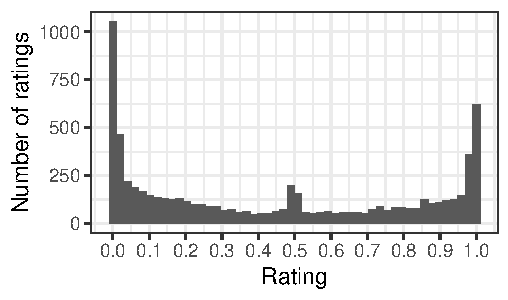
\includegraphics[width=\textwidth]{../../results/5-projectivity-no-fact/graphs/bunching}
\caption{Exp.~1a ratings.}
\label{fig:exp1araw}
\end{subfigure}
\begin{subfigure}{.33\textwidth}
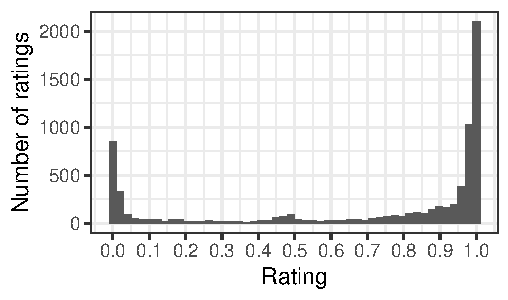
\includegraphics[width=\textwidth]{../../results/4-veridicality3/graphs/bunching}
\caption{Exp.~2a ratings.}
\label{fig:exp2araw}
\end{subfigure}
\begin{subfigure}{.33\textwidth}
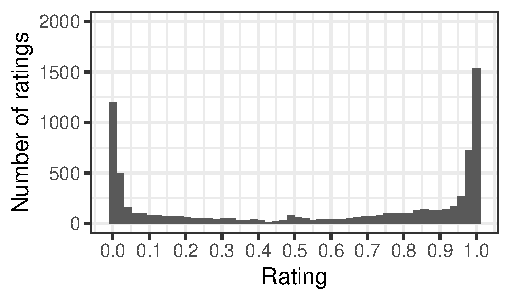
\includegraphics[width=\textwidth]{../../results/2-veridicality2/graphs/bunching}
\caption{Exp.~3a ratings.}
\label{fig:exp3araw}
\end{subfigure}
\caption{Histograms of raw slider ratings in Exps.~1a, 2a, and 3a.}
\label{fig:bunch}
\end{figure}

This ``bunching'' behavior, in turn, can lead to the violation of both of the above assumptions of linear regression. 
Intuitively, these assumptions are violated because conditions that elicit ratings closer to endpoints necessarily have a compressed variance; consequently, a condition's mean and its variance are not independent. Beta regression is useful here because it allows for modeling an arbitrarily distributed outcome variable in the $[$0,1$]$ interval. The Beta distribution is characterized by two parameters, one capturing the mean $\mu$ of the distribution and one capturing its precision $\phi$, a measure of dispersion. The greater the precision, the more concentrated the values are around the mean, i.e., the lower the variance of the distribution.  We follow \citet{smithson2006} in modeling $\mu$ and $\phi$ separately for each predictor. That is, we allow each predictor to affect both the mean and the precision of the outcome variable's distribution. 

\subsection{Coding choices and interpreting model output}\label{a-primer}

The outcome variable in Exps.~1a, 2a and 3a (slider ratings) contained the values 0 and 1, which Beta regression is undefined for. We therefore applied a common transformation to ratings before the main analysis that rescales values $y$ to fall in the open unit interval (0,1)  \citep{smithson2006}. First, we apply $y' = (y-a)/(b-a)$, where $b$ is the highest possible slider rating and $a$ is the smallest possible slider rating. The range is then compressed to not include 0 and 1 by applying $y'' = [y'(N-1) + 1/2]/N$, where $N$ is the total number of observations.

The mean parameter $\mu$ is modeled via a logit link function (default for Beta regression in \verb|brms|), though other links that squeeze $\mu$ into the $[$0,1$]$ interval are possible. The dispersion parameter $\phi$ is modeled via a log link, which ensures that values of $\phi$ are strictly positive, which is necessary because a variance cannot be negative. 

We allowed both $\mu$ and $\phi$ to vary as a function of predicate, with reference level set to main clause control in Exp.~1a, entailing control in Exp.~2a and contradictory control in Exp.~3a. We also allowed random intercept adjustments to each parameter by participant and by item, where item was defined as a unique combination of a predicate and a complement clause. Four chains converged after 2000 iterations each (warmup = 1000, \(\hat{R}=1\) for all estimated parameters) with a target acceptance rate of .95 and a maximum treedepth of 15.

\subsection{Model outputs for Experiments 1, 2 and 3}\label{a-mo}

The three tables in this section show the model outputs for Exps.~1, 2 and 3, respectively: Table \ref{tab:exp1modelresults} for Exps.~1a and 1b, Table \ref{tab:exp2modelresults} for Exps.~2a and 2b, and Table \ref{tab:exp3modelresults} for Exps.~3a and 3b. Each table shows maximum a posteriori (MAP) model estimates for certainty ratings from the Beta regression model (left and middle column, mean $\mu$ and precision $\phi$) and the logistic regression model (right column, $\beta$)  with 95\% credible intervals.

\begin{table}
\caption{Maximum a posteriori (MAP) model estimates for certainty ratings from Exp.~1a (left and middle column, mean $\mu$ and precision $\phi$) and Exp.~1b (right column, $\beta$)  with 95\% credible intervals. Contrast of each predicate is with main clause control reference level. MAP estimates for which there is no evidence that they are different from 0 are italicized.}
\small
\begin{center}
\begin{tabular}{l c c c}
\toprule
& \multicolumn{2}{c}{Exp.~1a: Beta regression} & Exp.~1b: logistic regression \\
Predictor & Estimated $\mu$ & Estimated $\phi$ & Estimated $\beta$\\
\midrule
\multirow{2}{*}{Intercept} & $-1.88 $  & $1.16 $ & $-6.37 $       \\
& $[-1.98;\ -1.78]$ & $[1.02;\ 1.29]$  & $[-7.10;\ -5.72]$ \\
[.25em]
\multirow{2}{*}{acknowledge} & $2.62 $ & $-0.67 $  & $8.00 $        \\
& $[2.45;\ 2.80]$  & $[-0.86;\ -0.49]$ & $[7.31;\ 8.78]$   \\
[.25em]
\multirow{2}{*}{admit} & $2.45 $ & $-0.65 $  & $7.29 $        \\
& $[2.29;\ 2.61]$  & $[-0.83;\ -0.48]$ & $[6.60;\ 8.04]$   \\
[.25em]
\multirow{2}{*}{announce}  & $2.14 $ & $-0.74 $  & $6.70 $        \\
& $[1.98;\ 2.30]$  & $[-0.92;\ -0.57]$ & $[6.04;\ 7.45]$   \\
[.25em]
\multirow{2}{*}{be annoyed} & $3.56 $ & $-0.30 $  & $9.41 $        \\
& $[3.37;\ 3.75]$  & $[-0.51;\ -0.10]$ & $[8.64;\ 10.22]$  \\
[.25em]
\multirow{2}{*}{be right} & $0.52 $ & $-0.21 $  & $2.33 $        \\
& $[0.36;\ 0.68]$  & $[-0.40;\ -0.01]$ & $[1.50;\ 3.21]$   \\
[.25em]
\multirow{2}{*}{confess} & $2.29 $ & $-0.71 $  & $6.75 $        \\
& $[2.13;\ 2.45]$  & $[-0.88;\ -0.54]$ & $[6.07;\ 7.50]$   \\
[.25em]
\multirow{2}{*}{confirm} & $1.31 $ & $-0.46 $  & $4.27 $        \\
& $[1.15;\ 1.46]$  & $[-0.64;\ -0.28]$ & $[3.60;\ 5.01]$   \\
[.25em]
\multirow{2}{*}{demonstrate} & $1.78 $ & $-0.59 $  & $5.31 $        \\
& $[1.63;\ 1.93]$  & $[-0.76;\ -0.41]$ & $[4.64;\ 6.06]$   \\
[.25em]
\multirow{2}{*}{discover}  & $2.90 $ & $-0.67 $  & $8.46 $        \\
& $[2.72;\ 3.07]$  & $[-0.85;\ -0.48]$ & $[7.75;\ 9.25]$   \\
[.25em]
\multirow{2}{*}{establish} & $1.42 $ & $-0.55 $  & $4.51 $        \\
& $[1.26;\ 1.58]$  & $[-0.73;\ -0.38]$ & $[3.83;\ 5.26]$   \\
[.25em]
\multirow{2}{*}{hear}  & $2.71 $ & $-0.79 $  & $8.22 $        \\
& $[2.53;\ 2.88]$  & $[-0.98;\ -0.61]$ & $[7.50;\ 9.01]$   \\
[.25em]
\multirow{2}{*}{inform}  & $3.00 $ & $-0.60 $  & $9.13 $        \\
& $[2.82;\ 3.18]$  & $[-0.79;\ -0.41]$ & $[8.38;\ 9.94]$   \\
[.25em]
\multirow{2}{*}{know}  & $3.37 $ & $-0.49 $  & $9.72 $        \\
& $[3.18;\ 3.56]$  & $[-0.70;\ -0.29]$ & $[8.94;\ 10.57]$  \\
[.25em]
\multirow{2}{*}{pretend} & $0.32 $ & $-0.19 $  & $3.22 $        \\
& $[0.15;\ 0.49]$  & $[-0.38;\ -0.00]$ & $[2.50;\ 4.03]$   \\
[.25em]
\multirow{2}{*}{prove} & $1.16 $ & $-0.21 $  & $3.92 $        \\
& $[1.01;\ 1.31]$  & $[-0.40;\ -0.03]$ & $[3.21;\ 4.67]$   \\
[.25em]
\multirow{2}{*}{reveal}  & $2.59 $ & $-0.72 $  & $7.41 $        \\
& $[2.42;\ 2.76]$  & $[-0.90;\ -0.55]$ & $[6.72;\ 8.16]$   \\
[.25em]
\multirow{2}{*}{say} & $0.78 $ & \emph{-0.12}  & $3.10 $        \\
& $[0.63;\ 0.93]$  & $[-0.30;\ 0.06]$ & $[2.35;\ 3.93]$   \\
[.25em]
\multirow{2}{*}{see} & $3.01 $ & $-0.70 $  & $8.74 $        \\
& $[2.83;\ 3.19]$  & $[-0.90;\ -0.51]$ & $[8.03;\ 9.55]$   \\
[.25em]
\multirow{2}{*}{suggest} & $0.79 $ & \emph{-0.17}  & $3.22 $        \\
& $[0.63;\ 0.94]$  & $[-0.36;\ 0.02]$ & $[2.49;\ 3.99]$   \\
[.25em]
\multirow{2}{*}{think} & $0.62 $ & \emph{0.01} & $2.54 $        \\
& $[0.47;\ 0.78]$  & $[-0.17;\ 0.20]$ & $[1.75;\ 3.40]$   \\
\bottomrule
\end{tabular}
\label{tab:exp1modelresults}
\end{center}
\end{table}

\normalsize


\begin{table}
\caption{Maximum a posteriori (MAP) model estimates for inference ratings from Exp.~2a (left and middle column, mean $\mu$ and precision $\phi$) and Exp.~2b (right column, $\beta$)  with 95\% credible intervals. Contrast of each predicate is with entailing control reference level. MAP estimates for which there is no evidence that they are different from 0 are italicized. Predicates are marked for which there is no evidence that they differ from  entailing controls (bold: no difference on either categorical or continuous measure; italics: no difference on at least one measure).}
\small
\begin{center}
\begin{tabular}{l c c c}
\toprule
& \multicolumn{2}{c}{Exp.~2a: Beta regression} & Exp.~2b: logistic regression \\
Predictor & Estimated $\mu$ & Estimated $\phi$ & Estimated $\beta$\\
\midrule
\multirow{2}{*}{Intercept}            & $3.00$        & $2.24$        & $6.20$          \\
                        & $[2.87;\ 3.15]$   & $[2.05;\ 2.42]$   & $[5.52;\ 6.98]$     \\
\multirow{2}{*}{acknowledge}      & $-0.74$       & $-0.64$       & $-1.58$         \\
                        & $[-0.94;\ -0.54]$ & $[-0.89;\ -0.39]$ & $[-2.47;\ -0.70]$   \\
\multirow{2}{*}{admit}            & $-0.67$       & $-0.52$       & $-1.83$         \\
                        & $[-0.87;\ -0.48]$ & $[-0.77;\ -0.27]$ & $[-2.72;\ -0.97]$   \\
\multirow{2}{*}{announce}         & $-1.51$       & $-1.35$       & $-4.39$         \\
                        & $[-1.71;\ -1.31]$ & $[-1.59;\ -1.10]$ & $[-5.17;\ -3.68]$   \\
\multirow{2}{*}{be annoyed}      & $-0.55$       & $-0.50$       & $-1.36$         \\
                        & $[-0.76;\ -0.35]$ & $[-0.75;\ -0.23]$ & $[-2.31;\ -0.46]$   \\
\multirow{2}{*}{\textbf{be right}}        & \emph{-0.03}           & \emph{0.09}            & \emph{0.36}              \\
                        & $[-0.22;\ 0.16]$  & $[-0.16;\ 0.34]$  & $[-0.93;\ 1.89]$    \\
\multirow{2}{*}{confess}          & $-0.85$       & $-0.64$       & $-2.79$         \\
                        & $[-1.05;\ -0.66]$ & $[-0.90;\ -0.38]$ & $[-3.60;\ -2.04]$   \\
\multirow{2}{*}{\emph{confirm}}          & $-0.22$       & \emph{-0.00}           & \emph{-0.85}             \\
                        & $[-0.41;\ -0.03]$ & $[-0.26;\ 0.26]$  & $[-1.84;\ 0.14]$    \\
\multirow{2}{*}{demonstrate}      & $-1.23$       & $-1.18$       & $-3.35$         \\
                        & $[-1.44;\ -1.02]$ & $[-1.44;\ -0.93]$ & $[-4.15;\ -2.63]$   \\
\multirow{2}{*}{\emph{discover}}         & $-0.27$       & \emph{-0.10}           & \emph{-0.50}             \\
                        & $[-0.46;\ -0.08]$ & $[-0.35;\ 0.14]$  & $[-1.57;\ 0.64]$    \\
\multirow{2}{*}{establish}        & $-0.78$       & $-0.68$       & $-1.92$         \\
                        & $[-0.98;\ -0.58]$ & $[-0.92;\ -0.42]$ & $[-2.76;\ -1.12]$   \\
\multirow{2}{*}{hear}             & $-2.92$       & $-2.05$       & $-7.57$         \\
                        & $[-3.12;\ -2.72]$ & $[-2.27;\ -1.83]$ & $[-8.41;\ -6.84]$   \\
\multirow{2}{*}{inform}           & $-1.37$       & $-1.29$       & $-3.93$         \\
                        & $[-1.57;\ -1.16]$ & $[-1.54;\ -1.05]$ & $[-4.71;\ -3.22]$   \\
\multirow{2}{*}{know}             & $-0.40$       & $-0.28$       & $-0.27$             \\
                        & $[-0.60;\ -0.21]$ & $[-0.54;\ -0.03]$ & $[-1.39;\ 0.96]$    \\
\multirow{2}{*}{nonMent.C}        & $-6.22$       & $-0.27$       & $-11.92$        \\
                        & $[-6.42;\ -6.02]$ & $[-0.52;\ -0.04]$ & $[-12.94;\ -11.01]$ \\
\multirow{2}{*}{pretend}          & $-4.47$       & $-2.13$       & $-10.78$        \\
                        & $[-4.72;\ -4.24]$ & $[-2.38;\ -1.87]$ & $[-11.83;\ -9.85]$  \\
\multirow{2}{*}{\textbf{prove}}            & \emph{-0.08}           & \emph{-0.13}           & \emph{0.92}              \\
                        & $[-0.29;\ 0.14]$  & $[-0.40;\ 0.14]$  & $[-0.57;\ 2.91]$    \\
\multirow{2}{*}{reveal}           & $-0.80$       & $-0.67$       & $-2.37$         \\
                        & $[-1.00;\ -0.60]$ & $[-0.92;\ -0.41]$ & $[-3.21;\ -1.54]$   \\
\multirow{2}{*}{say}              & $-2.20$       & $-1.92$       & $-5.79$         \\
                        & $[-2.41;\ -2.00]$ & $[-2.15;\ -1.69]$ & $[-6.59;\ -5.09]$   \\
\multirow{2}{*}{\emph{see}}              & $-0.23$       & \emph{-0.16}           & \emph{-0.49}             \\
                        & $[-0.43;\ -0.02]$ & $[-0.41;\ 0.09]$  & $[-1.51;\ 0.62]$    \\
\multirow{2}{*}{suggest}          & $-3.47$       & $-1.90$       & $-8.75$         \\
                        & $[-3.67;\ -3.27]$ & $[-2.12;\ -1.67]$ & $[-9.62;\ -7.95]$   \\
\multirow{2}{*}{think}            & $-3.64$       & $-1.85$       & $-9.71$         \\
                        & $[-3.84;\ -3.44]$ & $[-2.08;\ -1.62]$ & $[-10.65;\ -8.87]$  \\
\bottomrule
\end{tabular}
\label{tab:exp2modelresults}
\end{center}
\end{table}

\normalsize

\begin{table}
\caption{Maximum a posteriori (MAP) model estimates for contradictoriness ratings from Exp.~3a (left and middle column, mean $\mu$ and precision $\phi$) and Exp.~3b (right column, $\beta$)  with 95\% credible intervals. Contrast of each predicate is with contradictory control reference level. MAP estimates for which there is no evidence that they are different from 0 are italicized.}
\small
\begin{center}
\begin{tabular}{l c c c}
\toprule
& \multicolumn{2}{c}{Exp.~3a: Beta regression} & Exp.~3b: logistic regression \\
Predictor & Estimated $\mu$ & Estimated $\phi$ & Estimated $\beta$\\
\midrule
\multirow{2}{*}{Intercept}             & $2.74$        & $1.46$        & $6.17$          \\
                         & $[2.54;\ 2.93]$   & $[1.23;\ 1.66]$   & $[5.55;\ 6.88]$     \\
\multirow{2}{*}{acknowledge}       & $-2.15$       & $-1.04$       & $-4.89$         \\
                         & $[-2.39;\ -1.90]$ & $[-1.29;\ -0.79]$ & $[-5.65;\ -4.21]$   \\
\multirow{2}{*}{admit}             & $-2.03$       & $-1.05$       & $-4.86$         \\
                         & $[-2.26;\ -1.77]$ & $[-1.30;\ -0.78]$ & $[-5.59;\ -4.19]$   \\
\multirow{2}{*}{announce}          & $-2.90$       & $-1.56$       & $-6.46$         \\
                         & $[-3.14;\ -2.64]$ & $[-1.80;\ -1.32]$ & $[-7.20;\ -5.80]$   \\
\multirow{2}{*}{be annoyed}       & $-2.24$       & $-1.28$       & $-5.18$         \\
                         & $[-2.47;\ -1.98]$ & $[-1.53;\ -1.03]$ & $[-5.91;\ -4.51]$   \\
\multirow{2}{*}{be right}         & $-0.40$       & \emph{-0.18}           & $-1.90$         \\
                         & $[-0.67;\ -0.12]$ & $[-0.48;\ 0.12]$  & $[-2.70;\ -1.12]$   \\
\multirow{2}{*}{confess}           & $-2.15$       & $-1.12$       & $-4.85$         \\
                         & $[-2.39;\ -1.89]$ & $[-1.37;\ -0.86]$ & $[-5.59;\ -4.18]$   \\
\multirow{2}{*}{confirm}           & $-1.74$       & $-0.99$       & $-4.25$         \\
                         & $[-1.99;\ -1.48]$ & $[-1.24;\ -0.73]$ & $[-4.99;\ -3.57]$   \\
\multirow{2}{*}{demonstrate}       & $-1.94$       & $-1.05$       & $-4.53$         \\
                         & $[-2.18;\ -1.69]$ & $[-1.30;\ -0.79]$ & $[-5.25;\ -3.84]$   \\
\multirow{2}{*}{discover}          & $-1.63$       & $-1.02$       & $-3.30$         \\
                         & $[-1.90;\ -1.38]$ & $[-1.27;\ -0.75]$ & $[-4.06;\ -2.61]$   \\
\multirow{2}{*}{establish}         & $-1.94$       & $-1.00$       & $-4.29$         \\
                         & $[-2.19;\ -1.70]$ & $[-1.27;\ -0.75]$ & $[-5.06;\ -3.62]$   \\
\multirow{2}{*}{hear}              & $-3.72$       & $-1.29$       & $-8.98$         \\
                         & $[-3.97;\ -3.45]$ & $[-1.54;\ -1.01]$ & $[-9.79;\ -8.27]$   \\
\multirow{2}{*}{inform}            & $-2.78$       & $-1.51$       & $-6.46$         \\
                         & $[-3.03;\ -2.52]$ & $[-1.75;\ -1.25]$ & $[-7.20;\ -5.81]$   \\
\multirow{2}{*}{know}              & $-1.37$       & $-0.90$       & $-3.64$         \\
                         & $[-1.63;\ -1.11]$ & $[-1.17;\ -0.64]$ & $[-4.39;\ -2.95]$   \\
\multirow{2}{*}{non-contra.~control}      & $-5.26$       & \emph{-0.24}           & $-11.51$        \\
                         & $[-5.54;\ -4.98]$ & $[-0.51;\ 0.04]$  & $[-12.43;\ -10.71]$ \\
\multirow{2}{*}{pretend}           & $-3.72$       & $-1.35$       & $-8.97$         \\
                         & $[-3.98;\ -3.46]$ & $[-1.61;\ -1.10]$ & $[-9.78;\ -8.26]$   \\
\multirow{2}{*}{prove}             & $-1.18$       & $-0.71$       & $-3.36$         \\
                         & $[-1.44;\ -0.92]$ & $[-0.98;\ -0.45]$ & $[-4.10;\ -2.65]$   \\
\multirow{2}{*}{reveal}            & $-2.27$       & $-1.24$       & $-4.99$         \\
                         & $[-2.52;\ -2.02]$ & $[-1.50;\ -0.98]$ & $[-5.73;\ -4.32]$   \\
\multirow{2}{*}{say}               & $-3.17$       & $-1.51$       & $-7.11$         \\
                         & $[-3.42;\ -2.91]$ & $[-1.75;\ -1.25]$ & $[-7.87;\ -6.42]$   \\
\multirow{2}{*}{see}               & $-1.43$       & $-0.82$       & $-3.48$         \\
                         & $[-1.68;\ -1.18]$ & $[-1.08;\ -0.56]$ & $[-4.21;\ -2.78]$   \\
\multirow{2}{*}{suggest}           & $-3.58$       & $-1.17$       & $-8.92$         \\
                         & $[-3.83;\ -3.31]$ & $[-1.43;\ -0.92]$ & $[-9.71;\ -8.21]$   \\
\multirow{2}{*}{think}             & $-3.93$       & $-1.20$       & $-9.81$         \\
                         & $[-4.19;\ -3.66]$ & $[-1.47;\ -0.94]$ & $[-10.67;\ -9.06]$  \\
\bottomrule
\end{tabular}
\label{tab:exp3modelresults}
\end{center}
\end{table}

\normalsize


\section{Comparisons of gradient and categorical ratings}\label{a-comparison}

The Spearman rank correlation coefficient, a value between -1 and 1, is a nonparametric measure of rank correlation: the higher the coefficient, the more the relation between the the two variables can be described using a monotonic function; if the coefficient is positive, the value of one variable tends to increase with an increase in the other. For instance, in the case of our Exps.~1, a coefficient of 1 would mean that there is a perfectly monotone increasing relation between the ranking of the predicates in Exp.~1a and Exp.~1b: for any two predicates $p_1$ and $p_2$, if $p_1$ ranks below $p_2$ in Exp.~1a (that is, the mean certainty rating of $p_1$ is lower than that of $p_2$), then that ranking is preserved in Exp.~1b.

The three panels of Figure \ref{f-comparison} visualize the strong correlation between by-predicate mean ratings in Exps.~1a, 2a and 3a and by-predicate proportion of `yes' responses in Exps.~1b, 2b, and 3b, respectively.

\begin{figure}[h!]
\centering
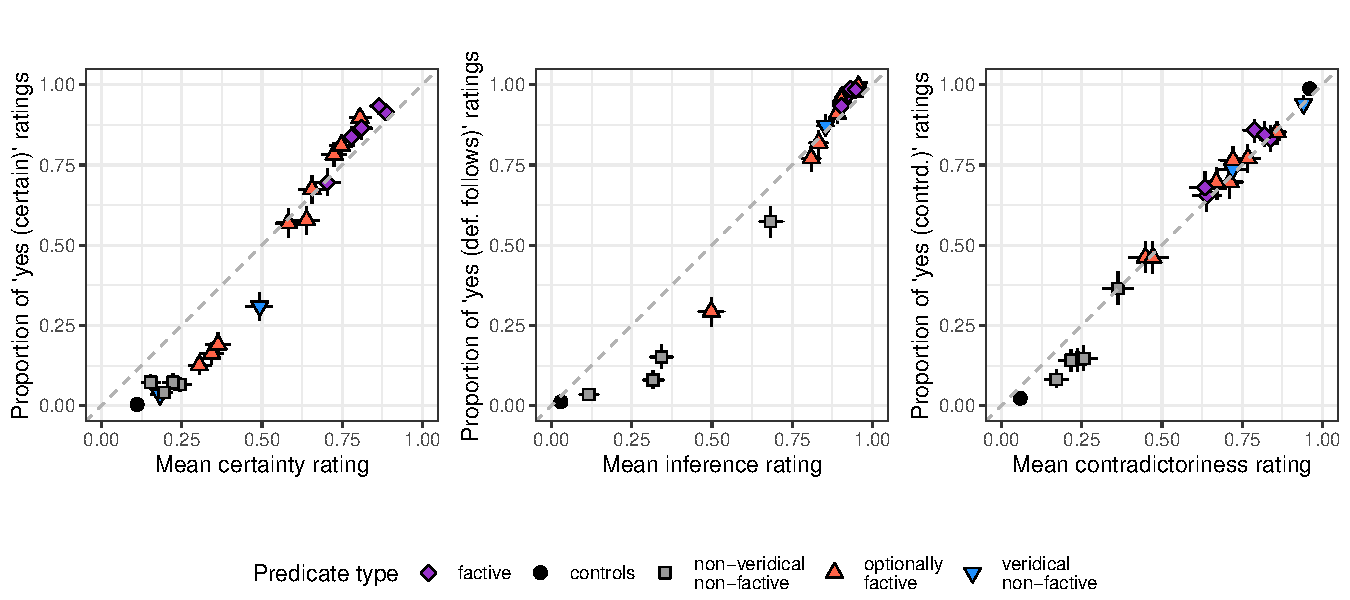
\includegraphics[width=.75\paperwidth]{../../results/compare-diagnostics-and-response-tasks/graphs/joint-comparison-plot}
   
\caption{By-predicate proportion of `yes' responses in two-alternative forced choice task against mean slider ratings in Exps.~1 (left, $r=.98$), Exps.~2 (middle, $r=.99$), and Exps.~3 (right, $r=.99$). Error bars indicate 95\% bootstrapped confidence intervals.}
\label{f-comparison}
\end{figure}


\end{document}

